\chapter{Background Determination}\label{ch:background}

This search is for signatures of large extra-dimensional signals, as described by the ADD model, producing a nonresonant excess of high-mass diphoton events above the SM diphoton background. A defining feature of this search is the approach used to determine its background---a technique yielding a full background prediction. The background arises from two components: the real background, which comes from prompt SM diphoton production; and the fake background, which occurs when jets are misidentified as a photons in the detector. The real background is dominant. This irreducible background is calculated using a next-to-next-to-leading order Monte Carlo calculation. The subdominant fake background is reducible and is estimated from control samples in data. 


\section{Background from SM Diphoton Production}\label{sec:real_background}

This analysis is searching for high-mass photon pairs in the region $\Mgg>500\GeV$. At the LHC, the dominant background in this search region arises from prompt SM diphoton production occurring through quark annihilation (the Born process) and gluon fusion (known as the ``box" process). The Born process dominants over the box process. The leading order (LO) Feynman diagrams for these processes are shown in Fig.~\ref{fig:sm_background_diagrams}. A $qg$-initiated process is also possible, as illustrated in Fig.~\ref{fig:NLO_pp}, but is formally higher order than the Born process and is suppressed compared to the box process due the large gluon parton distribution function (PDF), as discussed in the next section. The $\gamma\gamma$ final state of these processes is the same as the signal and, therefore, this real component of the background is irreducible. A next-to-next-to-leading order (NNLO) Monte Carlo calculation is used to determine the real background.

\begin{figure}[!htbp]
  \centering
  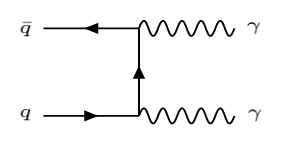
\includegraphics[scale=0.55]{figures/born}
  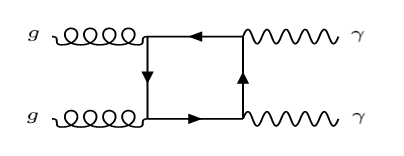
\includegraphics[scale=0.55]{figures/box}
  \caption{Representative Feynman diagrams for the LO SM diphoton Born (left) and box (right) processes.}
  \label{fig:sm_background_diagrams}
\end{figure}


\subsection{Monte Carlo Simulation}

Monte Carlo (MC) event generation in high-energy physics (a detailed review can be found in Section~41 of Ref.~\cite{Tanabashi:2018oca}) uses a divide and conquer philosophy. The phase space is typically split into distinct domains involving a matrix element (ME) and a parton shower (PS) calculation. The ME corresponds to the calculation of the hard interaction for specific particle processes. Cross section information is provided at this stage. The evolution of these parton-level processes through radiation and fragmentation is then handled in the PS calculation. A full event history of each particle is obtained by merging the two spaces. As quarks and gluons emerge from the collisions, they radiate gluons, which split into quark-antiquark pairs. This splitting process is known as fragmentation and is dominated by the emission of soft and collinear radiation until the scale $\Lambda_{\mathrm{QCD}}$ is reached and the partons become confined into hadrons, a process known as hadronization. Hadronization is a non-perturbation process, described by different phenomenological models. For the real background calculation, we use \SHERPA~v.2.1.1~\cite{Gleisberg:2008ta}, a full Monte Carlo (MC) event generator capable of performing these steps. \SHERPA incorporates the cluster model~\cite{Webber:1983if,Winter:2003tt} to describe hadronization. To characterize the LHC proton-proton collisions, \SHERPA is embedded with the CT10 set of PDFs~\cite{Lai:2010vv,Gao:2013xoa}.

The PDF allows us to assign a fraction $x$, called the the Bjorken $x$ variable, of the total proton momentum to the colliding partons within each proton. The PDF $f_{a/A}(x_a,\mu_f^2)$ describes the probability that a parton $a$ within some hadron $A$ carries the fraction $x_a$ of the total hadron momentum, where $\mu_f$ is the factorization scale, which, roughly, separates the long- and short-distance processes. Recall, that at short distances, or equivalently high energies, QCD is perturbative, allowing these processes to be calculated, while at long distances the regime is non-perturbative. The factorization scale is usually set at the energy scale of the hard scattering interaction, $\mu_f \sim Q^2$, where $Q^2$ is the momentum transfer in the collision. The interaction cross section is found by summing over the partons and integrating the PDFs according to:
\begin{equation}
  \sigma_{AB\to X} = \sum_{a,b} \int{dx_a dx_b f_{a/A}(x_a,\mu_f^2) f_{b/B}(x_b,\mu_f^2) } \hat{\sigma}_{ab\to X}
\end{equation}
\noindent for partons $a$ and $b$, within hadrons $A$ and $B$, carrying momentum fractions $x_a$ and $x_b$, respectively, where $\hat{\sigma}_{ab\to X}$ is the parton hard scattering cross section. See Fig.~\ref{fig:pp_collision} for a diagram representing this hard scattering process. In addition to $\mu_f$, this calculation also requires the choice of the renormalization scale $\mu_r$, the scale for the QCD running coupling. Some example PDFs from the CT10 PDF set are shown in Fig.~\ref{fig:ct10_pdf}.

\begin{figure}[!htbp]
  \centering
  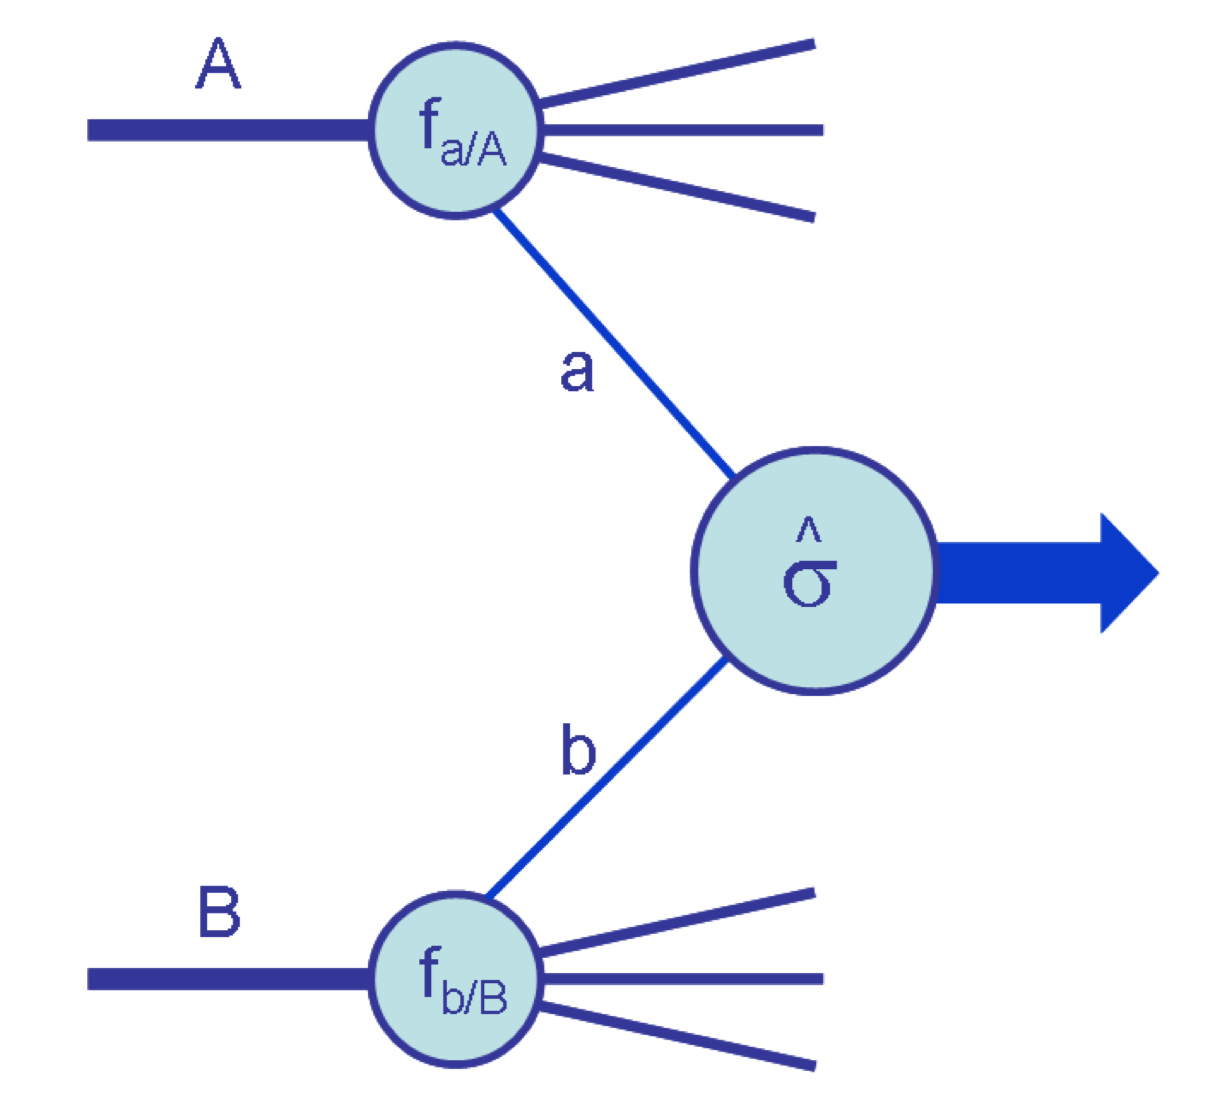
\includegraphics[scale=0.35]{figures/pp_collision}
  \caption{Diagrammatic representation of a proton-proton collision with their partons undergoing the hard scattering process~\cite{Campbell:2006wx}. The remainder of the two protons after collision is known as the beam remnant.}
  \label{fig:pp_collision}
\end{figure}

\begin{figure}[!htbp]
  \centering
  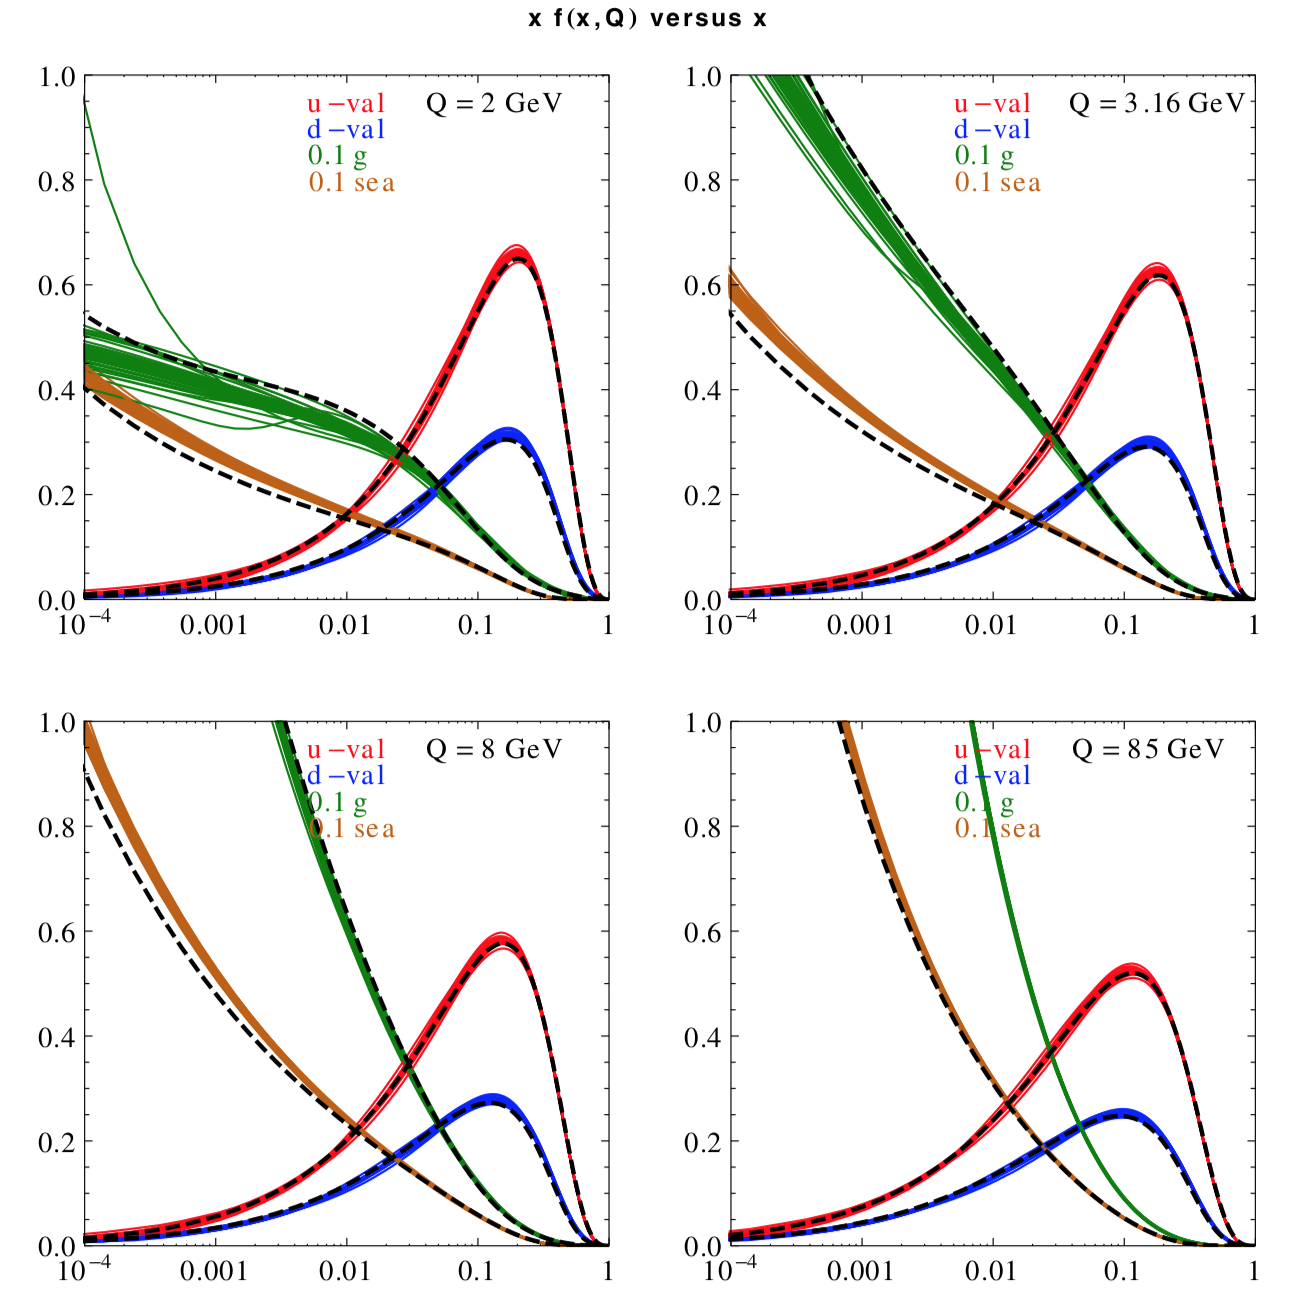
\includegraphics[scale=0.50]{figures/ct10_pdf}
  \caption{Example PDFs at energy scales $Q=2$, 3.16, 8, and 85\GeV, from the CT10 set of PDFs~\cite{Gao:2013xoa}.}
  \label{fig:ct10_pdf}
\end{figure}

\SHERPA can be configured to produced events from user specified processes generated from the proton collisions. Both the Born and box processes are included in the \SHERPA ME calculation and treated separately. The box process is calculated at the LO 1-loop level using a dedicated loop-induced ME generator. Even though the box process is formally NNLO, its contribution to the cross section is comparable to the LO terms due to the large gluon PDFs. Up to three additional final state partons are included in the Born process. Both quarks and gluons are allowed in the initial state of the Born process yielding higher order terms involving the additional final state partons through $jj\to\gamma\gamma+nj$, for a jet $j$ and integer $n=0$, 1, 2, or 3. However, \SHERPA only incorporates the real radiation component of these higher order processes and does not include virtual corrections. Fig.~\ref{fig:NLO_pp} shows some representative Feynman diagrams for NLO diphoton production in the Born process. 

\begin{figure}[hbt!]
  \centering
  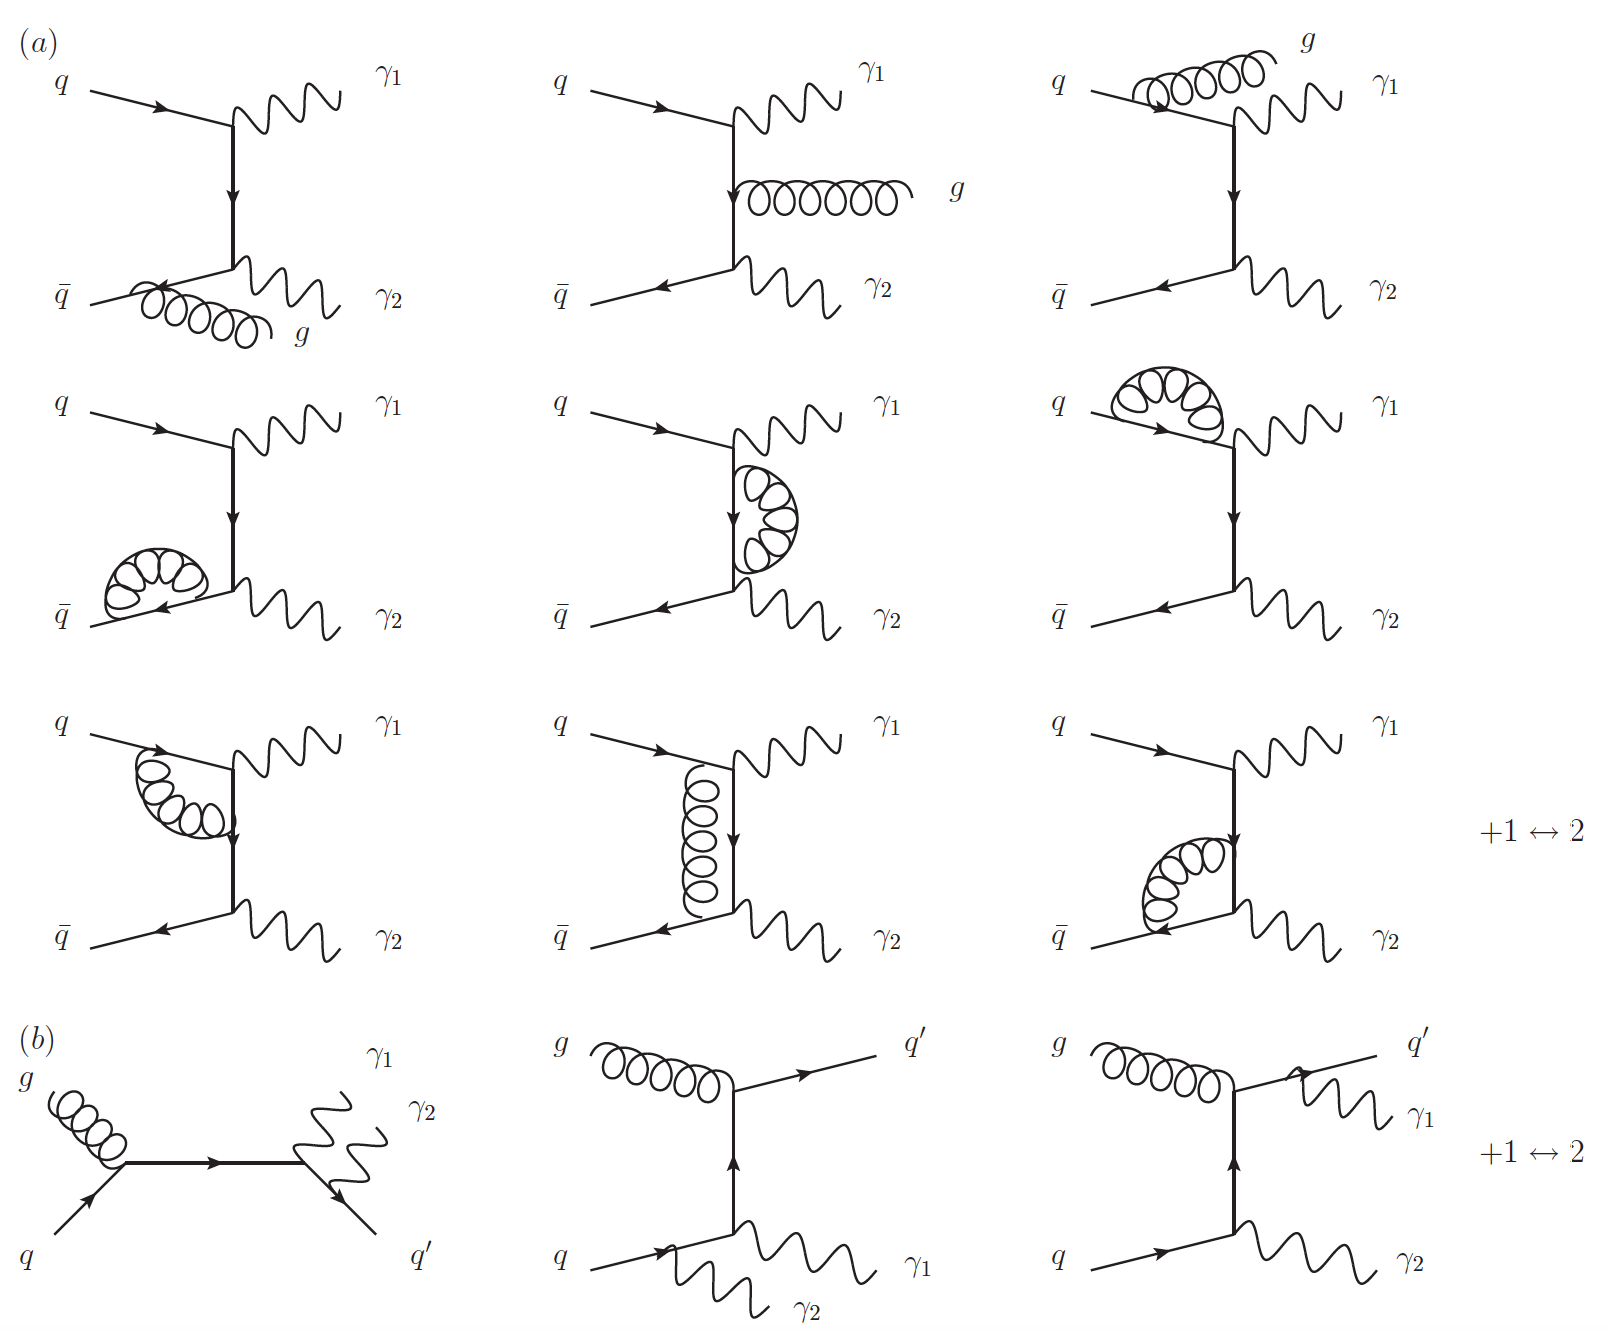
\includegraphics[scale=0.55]{figures/born_nlo}
  \caption{Representative Feynman diagrams for NLO diphoton production through the born process~\cite{DErrico:2011cgc}. In (a) $q\bar{q}$ and (b) $gq$ initiated processes are shown.}
  \label{fig:NLO_pp}
\end{figure}

The inclusion of additional final state jets is important for sampling the diphoton phase space as demonstrated in Ref.~\cite{CMS-PAS-EXO-12-045}. Here it was determined using Run 1 data that the variable $\Delta\phi_{\gamma\gamma}$, which is the difference in the $\phi$ coordinate between the two photons forming the diphoton object in the event, is sensitive to the presence of these additional jets and using a LO simulation was insufficient at accurately calculating the process. For computational convenience, the probability for producing these higher order processes is altered within \SHERPA by applying weights to the additional final state partons. This is corrected for in the final analysis by extracting the weights and undoing them when incorporating this background calculation. In addition to these specific processes, \SHERPA also interlaces photons into the QCD\texttt{+}QED PS~\cite{Hoeche:2009xc}. This provides prompt photon contributions from the fragmentation of quarks and gluons and is taken into account when estimating the fake background. Representative Feynman diagrams for this fragmentation process are shown in Fig.~\ref{fig:NLO_pp_onefrag}.

\begin{figure}[!htbp]
  \centering
  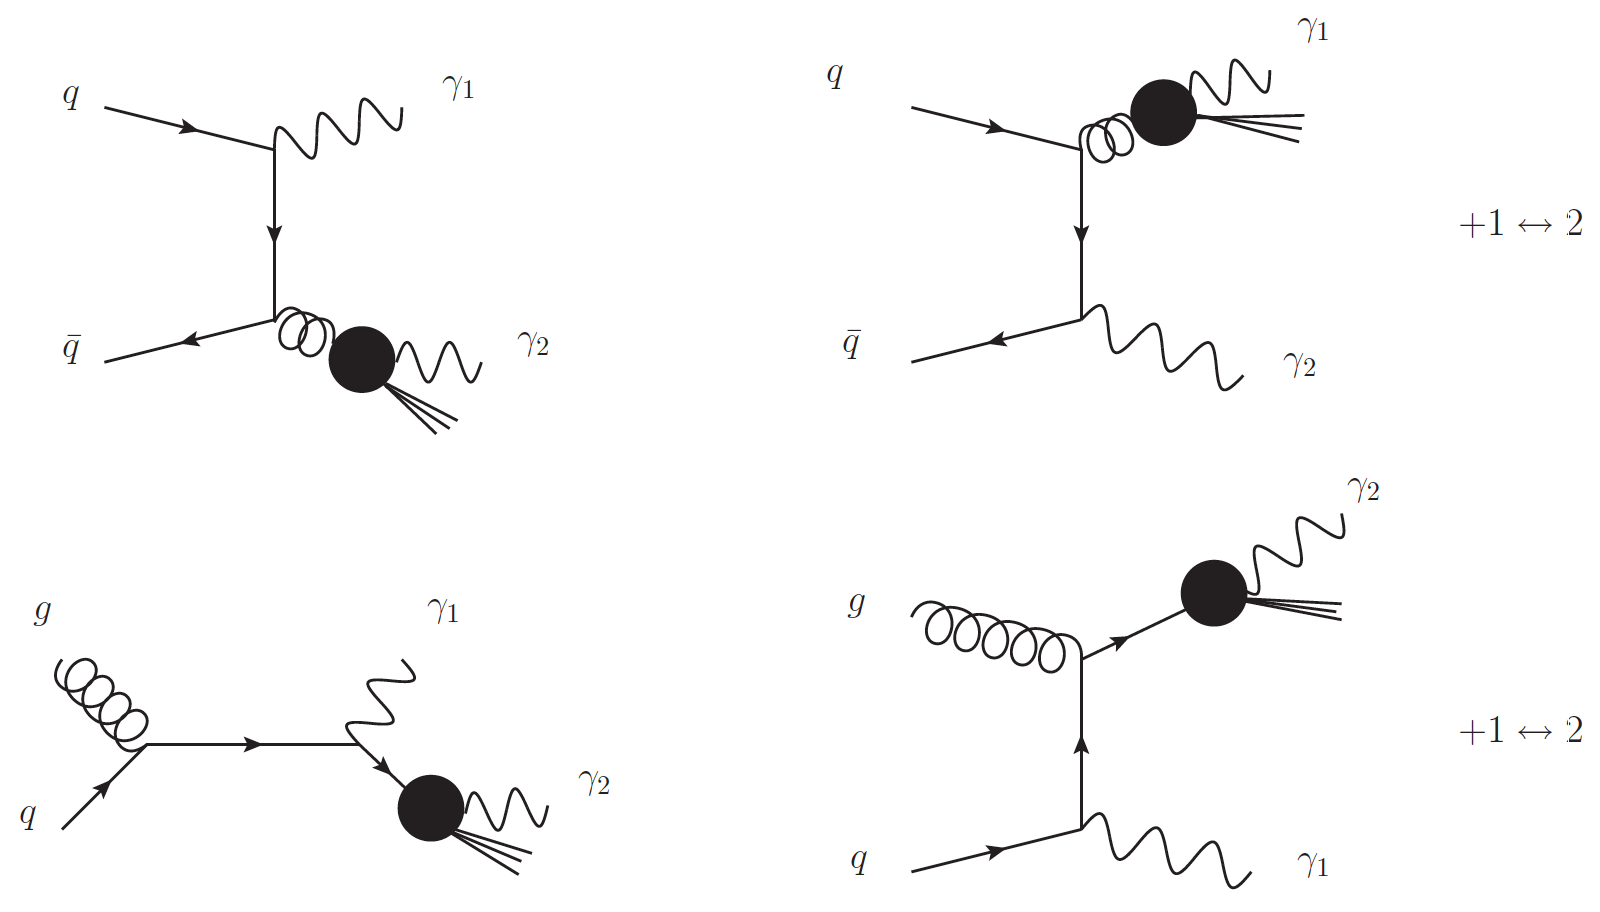
\includegraphics[scale=0.45]{figures/born_frag}
  \caption{Representative Feynman diagrams for NLO diphoton production through the fragmentation of a quark or gluon~\cite{DErrico:2011cgc}.}
  \label{fig:NLO_pp_onefrag}
\end{figure}

Within \SHERPA a kinematic selection of $\pt>50\GeV$ and $|\eta|<2.8$ is imposed on the photons during event generation. To improve statistics the event generation is broken into eight samples corresponding to the diphoton invariant mass \Mgg bins of 60-200, 200-500, 500-1000, 1000-2000, 2000-4000, 4000-6000, 6000-8000, and 8000-13000\GeV. These parameters are specified and configured in \SHERPA using run cards. An example run card used to generate one of these samples is shown in Appendix~\ref{sec:SM_run_card}. Among all samples, a total of 6,150,000 events were generated. Table~\ref{tab:ggjets_samples} summarizes the samples and their corresponding cross sections. For each sample, the interactions of the generated particles are fully simulated through the CMS detector material using \GEANTfour~\cite{Agostinelli:2002hh} and their response to the detector's electronic readout is then reconstructed. The simulation and reconstruction use CMS detector conditions that match those used during the 2016 data-taking period and include the effects of pileup from the proton-proton collisions.

\begin{table}[!htbp]
  \caption{MC background samples used in this analysis with the number of events and corresponding cross sections. The full, internal CMS path name is specified by appending the dataset path with \texttt{/RunIISummer16MiniAODv2-\allowbreak PUMoriond17\_\allowbreak 80X\_\allowbreak mcRun2\_\allowbreak asymptotic\_\allowbreak 2016\_\allowbreak TrancheIV\_\allowbreak v6/\allowbreak MINIAODSIM}.}
  \label{tab:ggjets_samples}
  \centering
  \vspace{\baselineskip}
  \begin{tabular}{lcc}
    \hline
    \hline
    Dataset path & Number of events & Cross section (pb) \\
    \hline
    /GGJets\_M-60To200\_Pt-50\_13TeV-sherpa     & 1,000,000 & 5.785     \\
    /GGJets\_M-200To500\_Pt-50\_13TeV-sherpa    & 2,500,000 & 2.244     \\
    /GGJets\_M-500To1000\_Pt-50\_13TeV-sherpa   & 1,000,000 & 1.510     \\
    /GGJets\_M-1000To2000\_Pt-50\_13TeV-sherpa  & 600,000   & 1.084e-02 \\
    /GGJets\_M-2000To4000\_Pt-50\_13TeV-sherpa  & 300,000   & 3.690e-04 \\
    /GGJets\_M-4000To6000\_Pt-50\_13TeV-sherpa  & 300,000   & 2.451e-06 \\
    /GGJets\_M-6000To8000\_Pt-50\_13TeV-sherpa  & 250,000   & 1.753e-08 \\
    /GGJets\_M-8000To13000\_Pt-50\_13TeV-sherpa & 200,000   & 7.053e-11 \\
    \hline
    \hline
  \end{tabular}
\end{table}

\correction{These \SHERPA samples contain individual events which have been fully simulated and reconstructed through the CMS detector, but higher order terms are absent. Unfortunately, at present, the MC programs capable of calculating the SM diphoton background at higher orders are not interfaced with \GEANTfour and, hence, cannot provide simulated events. However, these higher order MC programs are capable of calculating (currently, at full NNLO) the diphoton cross section at generator-level in a specified phase space, yielding distributions. \SHERPA also provides these same distributions at generator-level, allowing for a comparison. The ratio of these generator-level background predictions is called the \Kfactor. We will follow this general approach to produce a \Kfactor which will be subsequently applied to the simulation-level \SHERPA samples. This procedure allows us to reweight the simulated events, providing a full NNLO diphoton background prediction, accounting for the missing higher order terms in the original samples.}


\subsection{The \emph{K} Factor}\label{sec:k_factor}


\correction{The MC program \MCFM~8.0~\cite{Campbell:2016yrh} is capable of calculating a full NNLO diphoton cross section at generator-level and will be used to form the \Kfactor. \MCFM includes the 1-loop virtual corrections to the Born process, as shown in Fig.~\ref{fig:NLO_pp}, as well as for the box process. In addition, \MCFM includes the NNLO diagrams for the Born process and NLO diagrams for the box process in its calculation, as depicted in Figures~\ref{fig:MCFM_born_diagrams} and~\ref{fig:MCFM_box_diagrams}, respectively. \MCFM allows light fermions in the box process to circulate in the loop, but further considers the finite mass of the $t$ quark by also allowing it to circulate. The effects of this become important at high \Mgg~~\cite{Campbell:2016yrh}.}

\begin{figure}[hbt!]
  \centering
  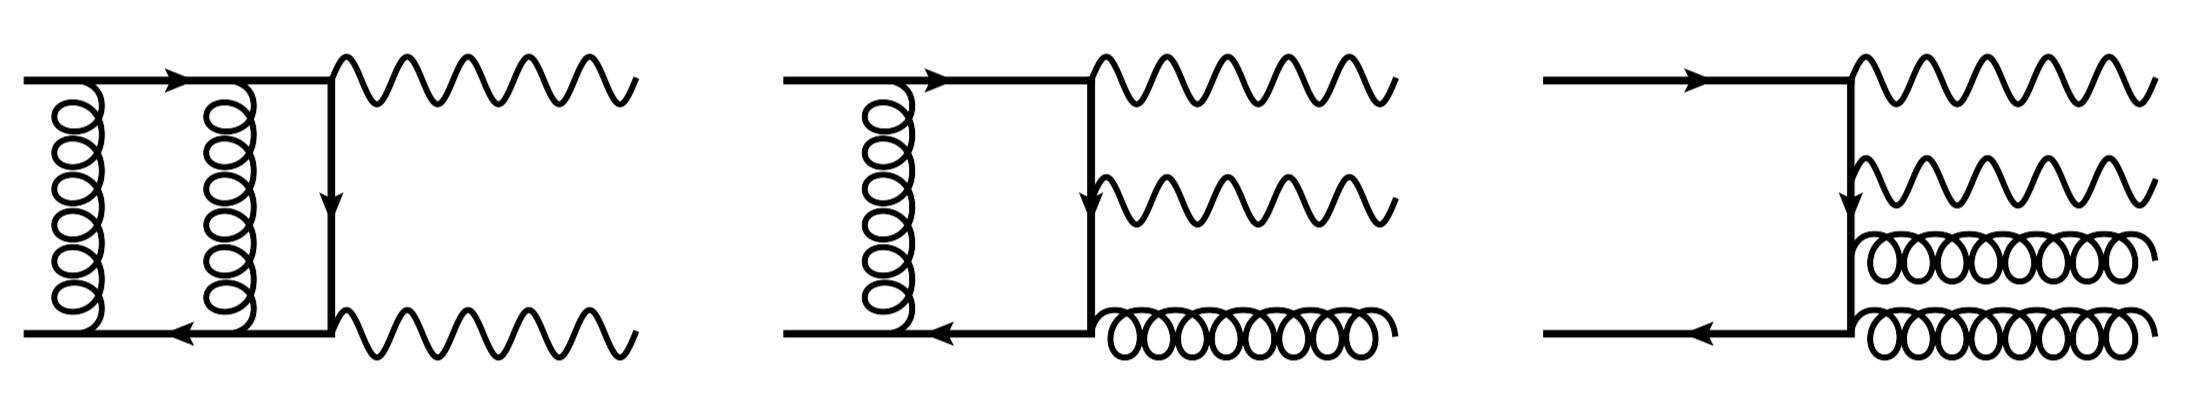
\includegraphics[scale=0.40]{figures/born_nnlo}
  \caption{Representative Feynman diagrams for the diphoton Born process at NNLO, considered by \MCFM~\cite{Campbell:2016yrh}.}
  \label{fig:MCFM_born_diagrams}
\end{figure}

\begin{figure}[hbt!]
  \centering
  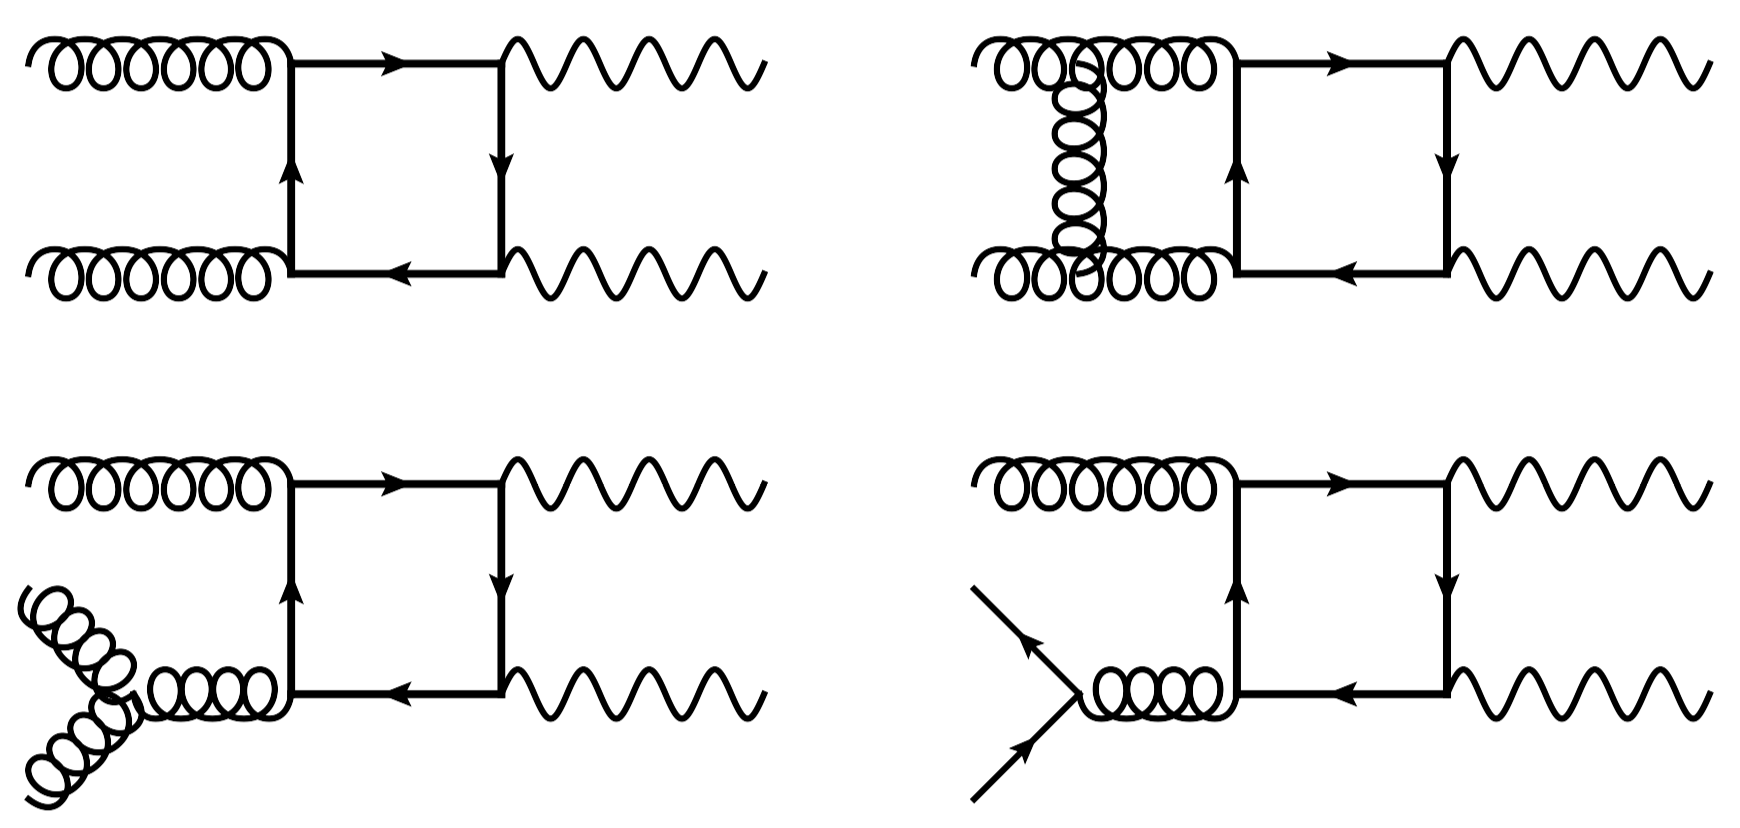
\includegraphics[scale=0.50]{figures/box_nlo}
  \caption{Representative Feynman diagrams for the diphoton box process at LO and NLO, considered by \MCFM~\cite{Campbell:2016yrh}.}
  \label{fig:MCFM_box_diagrams}
\end{figure}

\correction{For the calculation, we will interface \MCFM with the CT10 set of PDFs, as was done for the \SHERPA calculation. \MCFM can only provide parton-level cross section information for different diphoton kinematic variables, instead of individual, simulation-level events, since it is not interfaced with \GEANTfour. The NNLO contributions to the SM diphoton production processes are calculated as functions of \Mgg. Kinematic cuts are placed on the generator-level photons during the parton-level calculation. These are the same kinematic cuts used offline in the analysis, requiring photons to have $\pt>75\GeV$ and restricting them to reside within the EB or an EE using the appropriate values of photon $\eta$. Photon isolation is calculated using the method by Frixione~\cite{Frixione:1998jh}, which imposes an isolation requirement that depends on the $\Delta R$ from the location of the photon. The isolation at all distances must be within 5\GeV. Diphoton objects are then selected and categorized into the EBEB and EBEE regions. The four \Mgg bins of 500-750, 750-1000, 1000-1500, and 1500-4000\GeV are used during the calculation to improve the statistics of the overall calculation and reduce any potential statistical bias when a large range of \Mgg is separately considered. Finally, we reject events with very small $\Delta R_{\gamma\gamma}$ ($<$0.45) to avoid an infrared divergence from collinear photon emissions. \SHERPA is configured in an analogous way, providing similar diphoton cross section distributions as a function of \mgg, allowing for the formation of the \Kfactor.}

\correction{The \Kfactor is defined as the ratio of the \MCFM NNLO generator-level prediction to the \SHERPA generator-level prediction, both produced using equivalent settings. Fig.~\ref{fig:kfactor_mgg} (middle) shows the \MCFM LO (black), NLO (blue), and NNLO (red) calculations as a function of \Mgg compared against the \SHERPA generator-level prediction (magenta). The ratio plots show the \Kfactor distributions for each order with the final NNLO \Kfactor shown in red. The \Kfactor ranges from 1.4 to 2.2 (2.5) in the EBEB (EBEE) region for $\Mgg<3\TeV$.}

\begin{figure}[p]
  \centering
  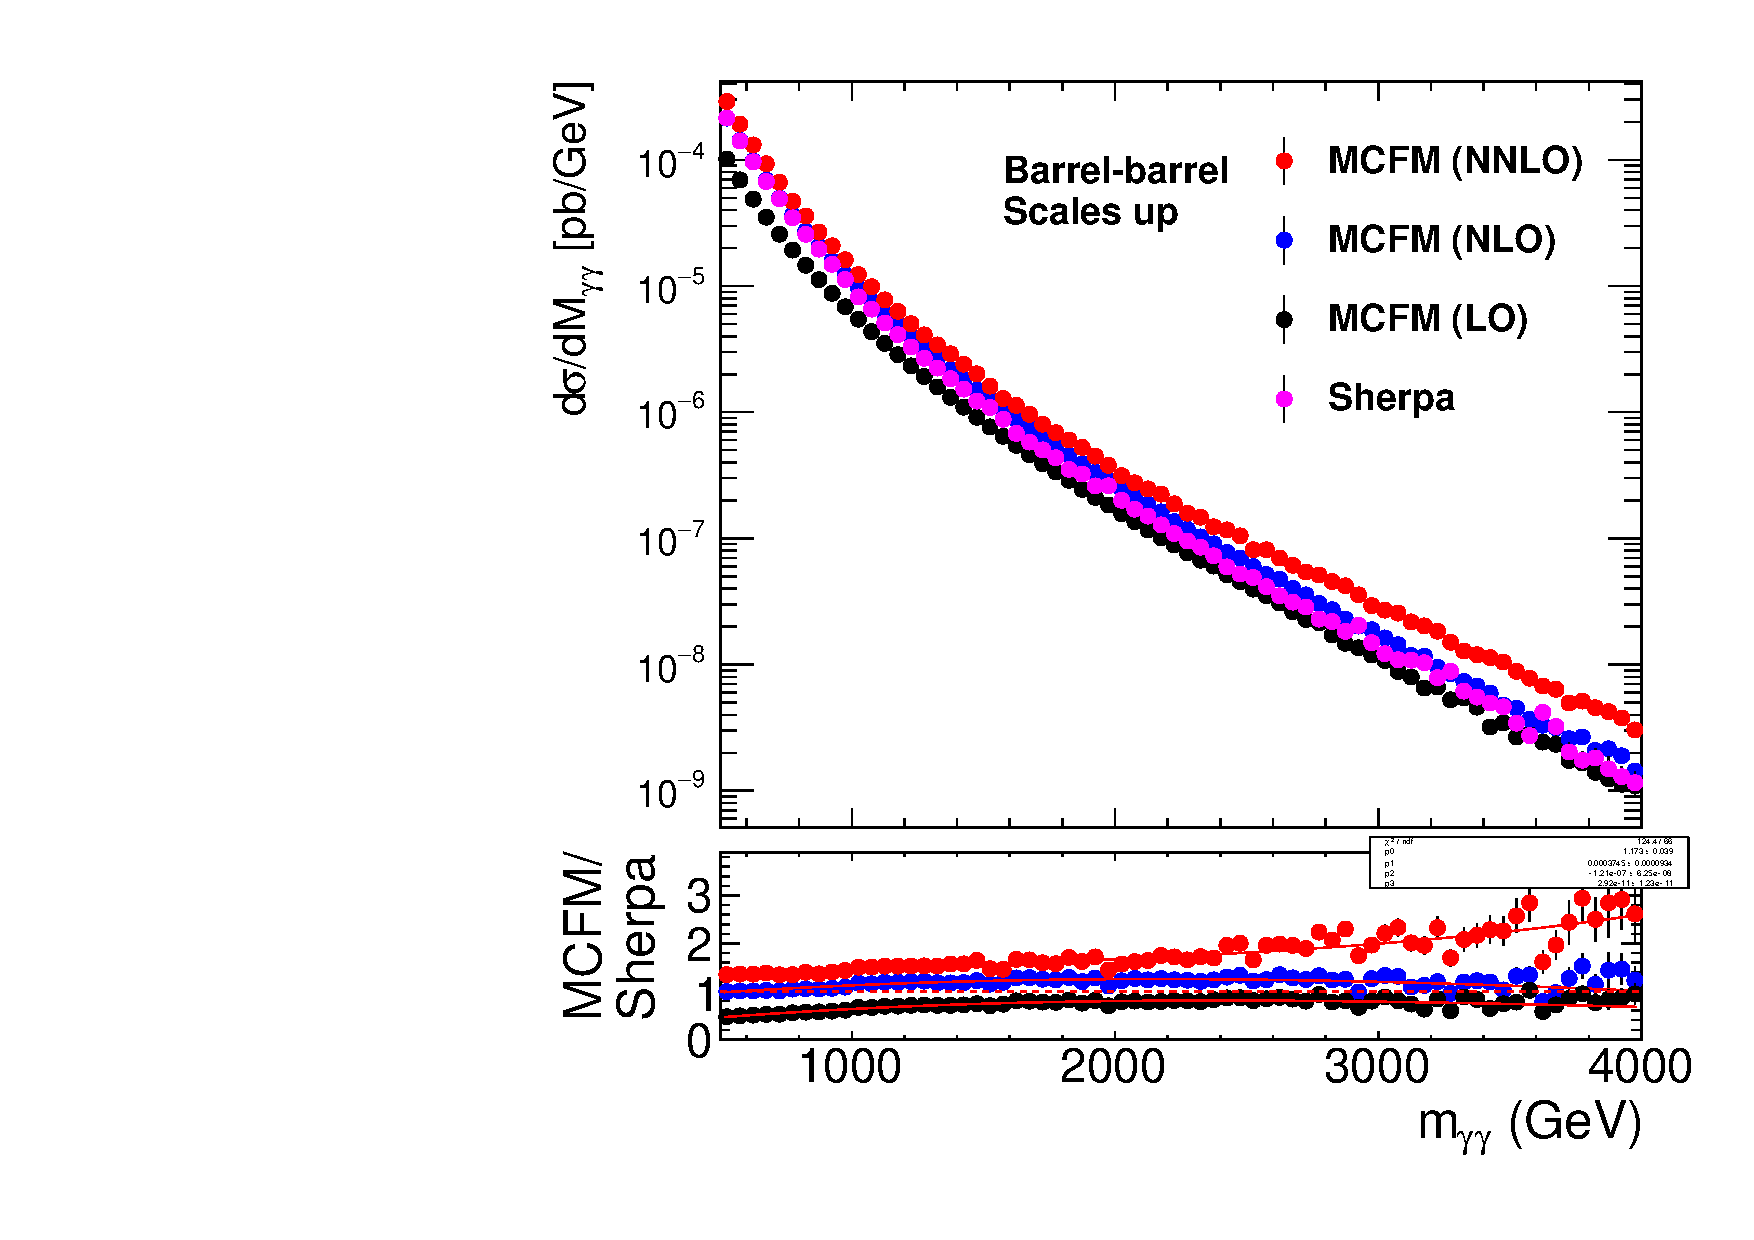
\includegraphics[angle=0,width=0.40\textwidth]{figures/BB_hist1_R2F2.pdf}
  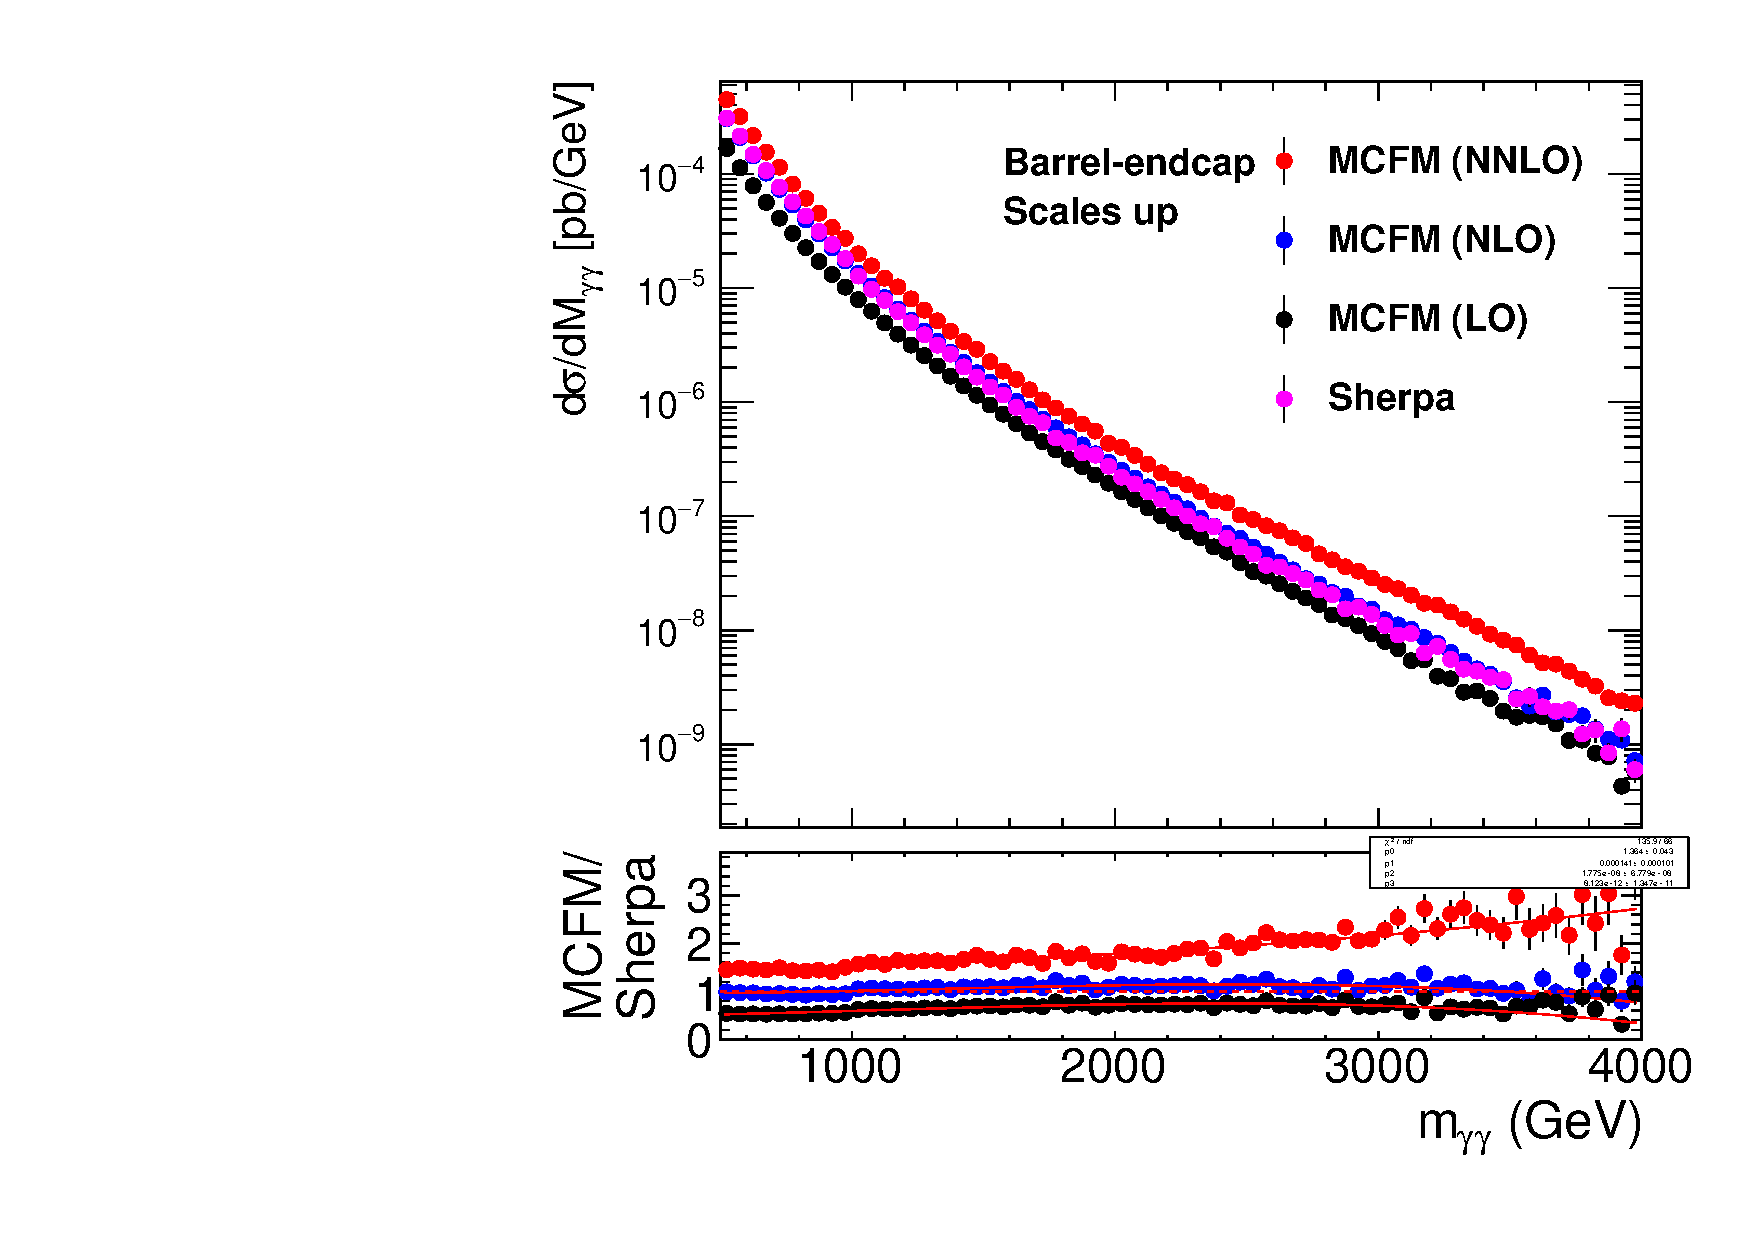
\includegraphics[angle=0,width=0.40\textwidth]{figures/BE_hist1_R2F2.pdf}
  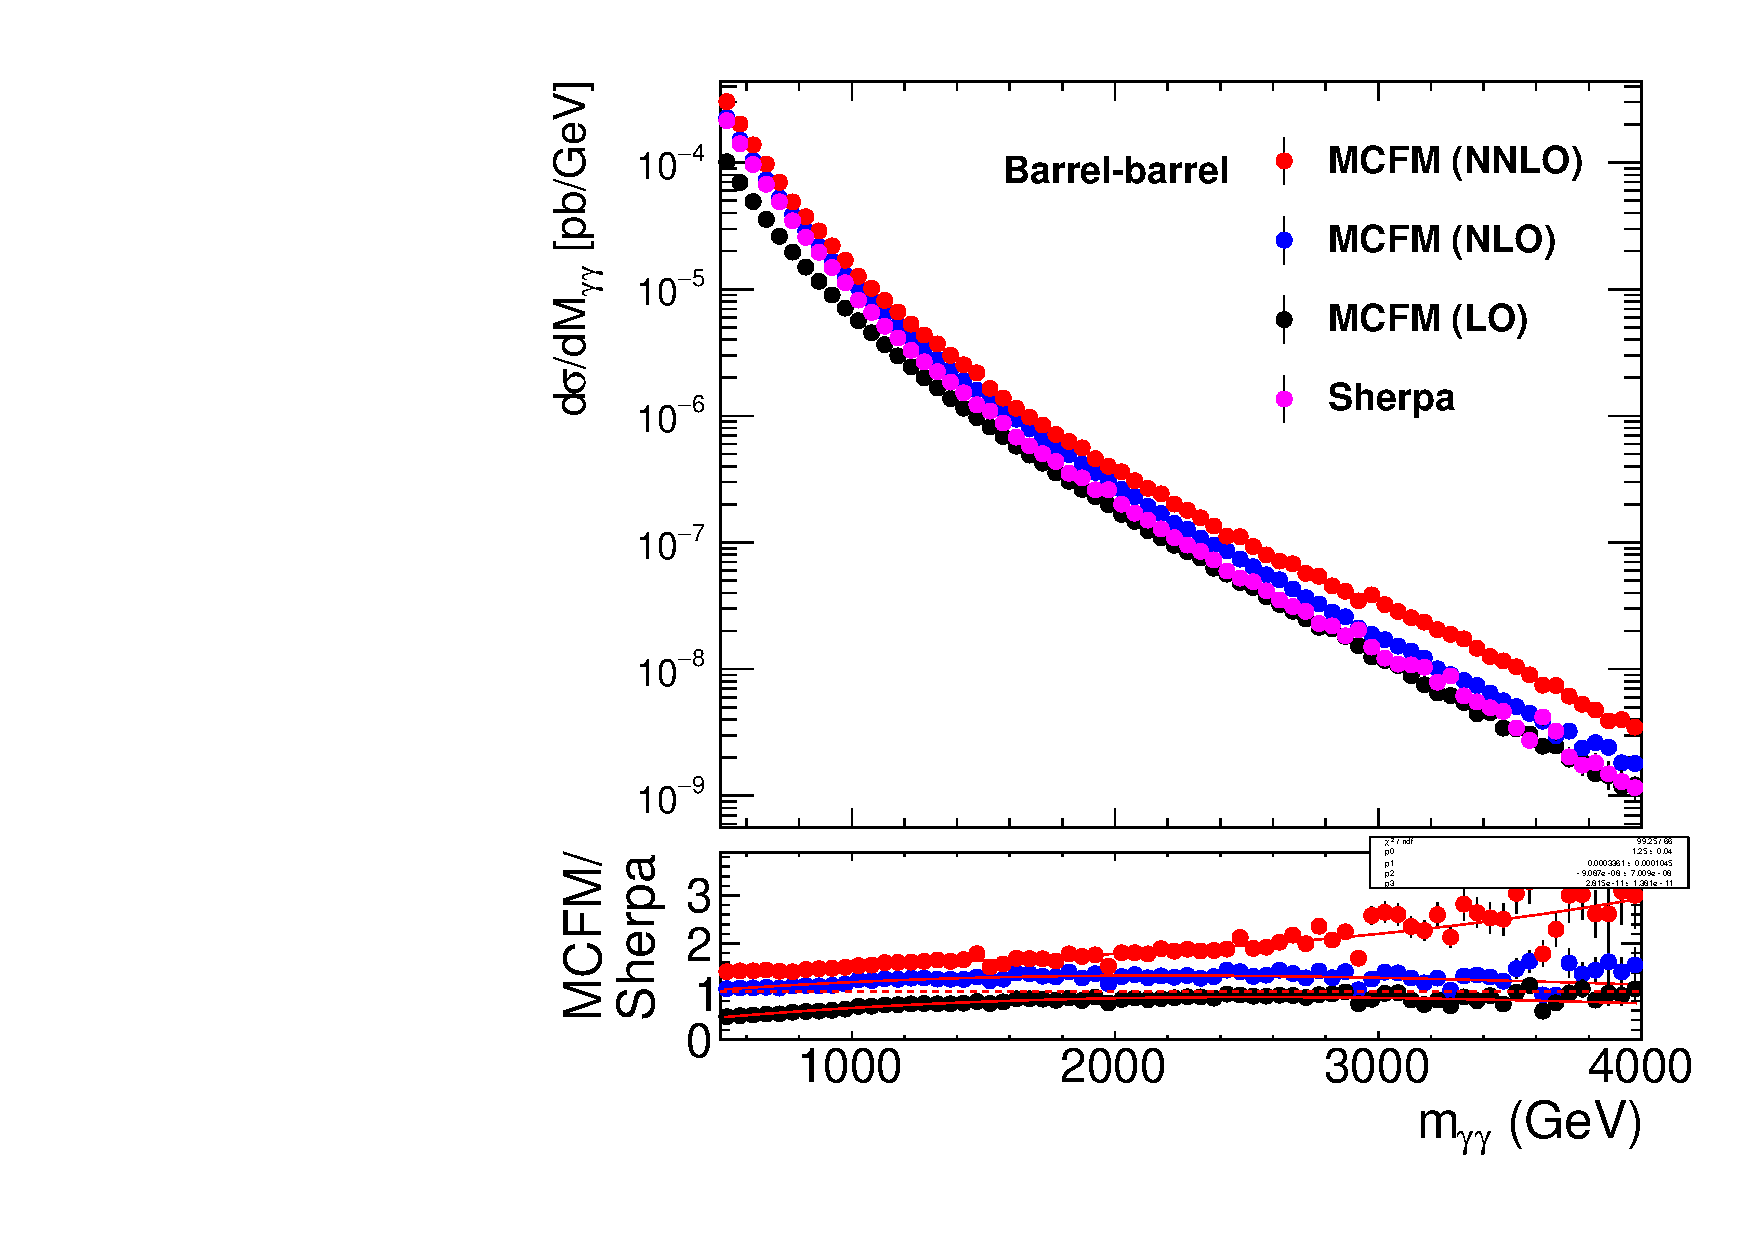
\includegraphics[angle=0,width=0.40\textwidth]{figures/BB_hist1_R1F1.pdf}
  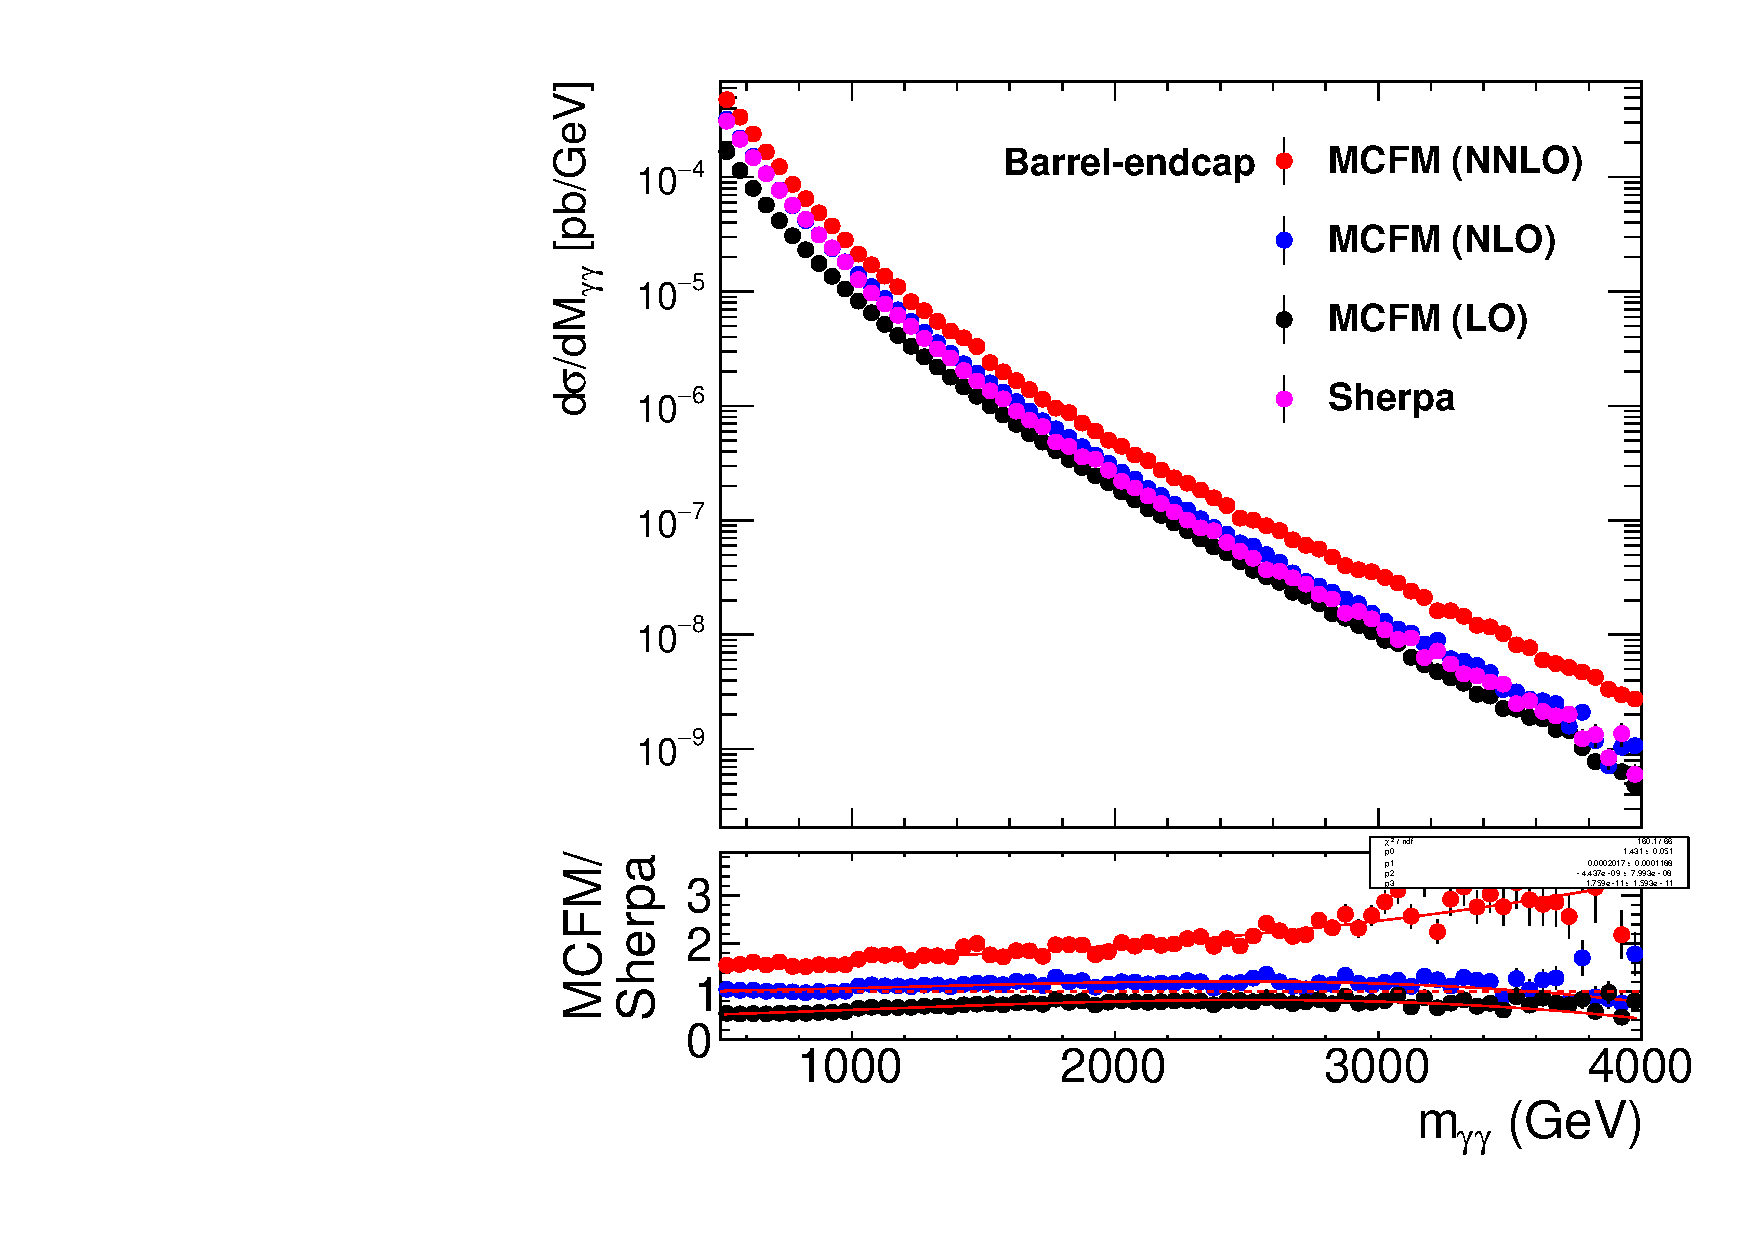
\includegraphics[angle=0,width=0.40\textwidth]{figures/BE_hist1_R1F1.pdf}
  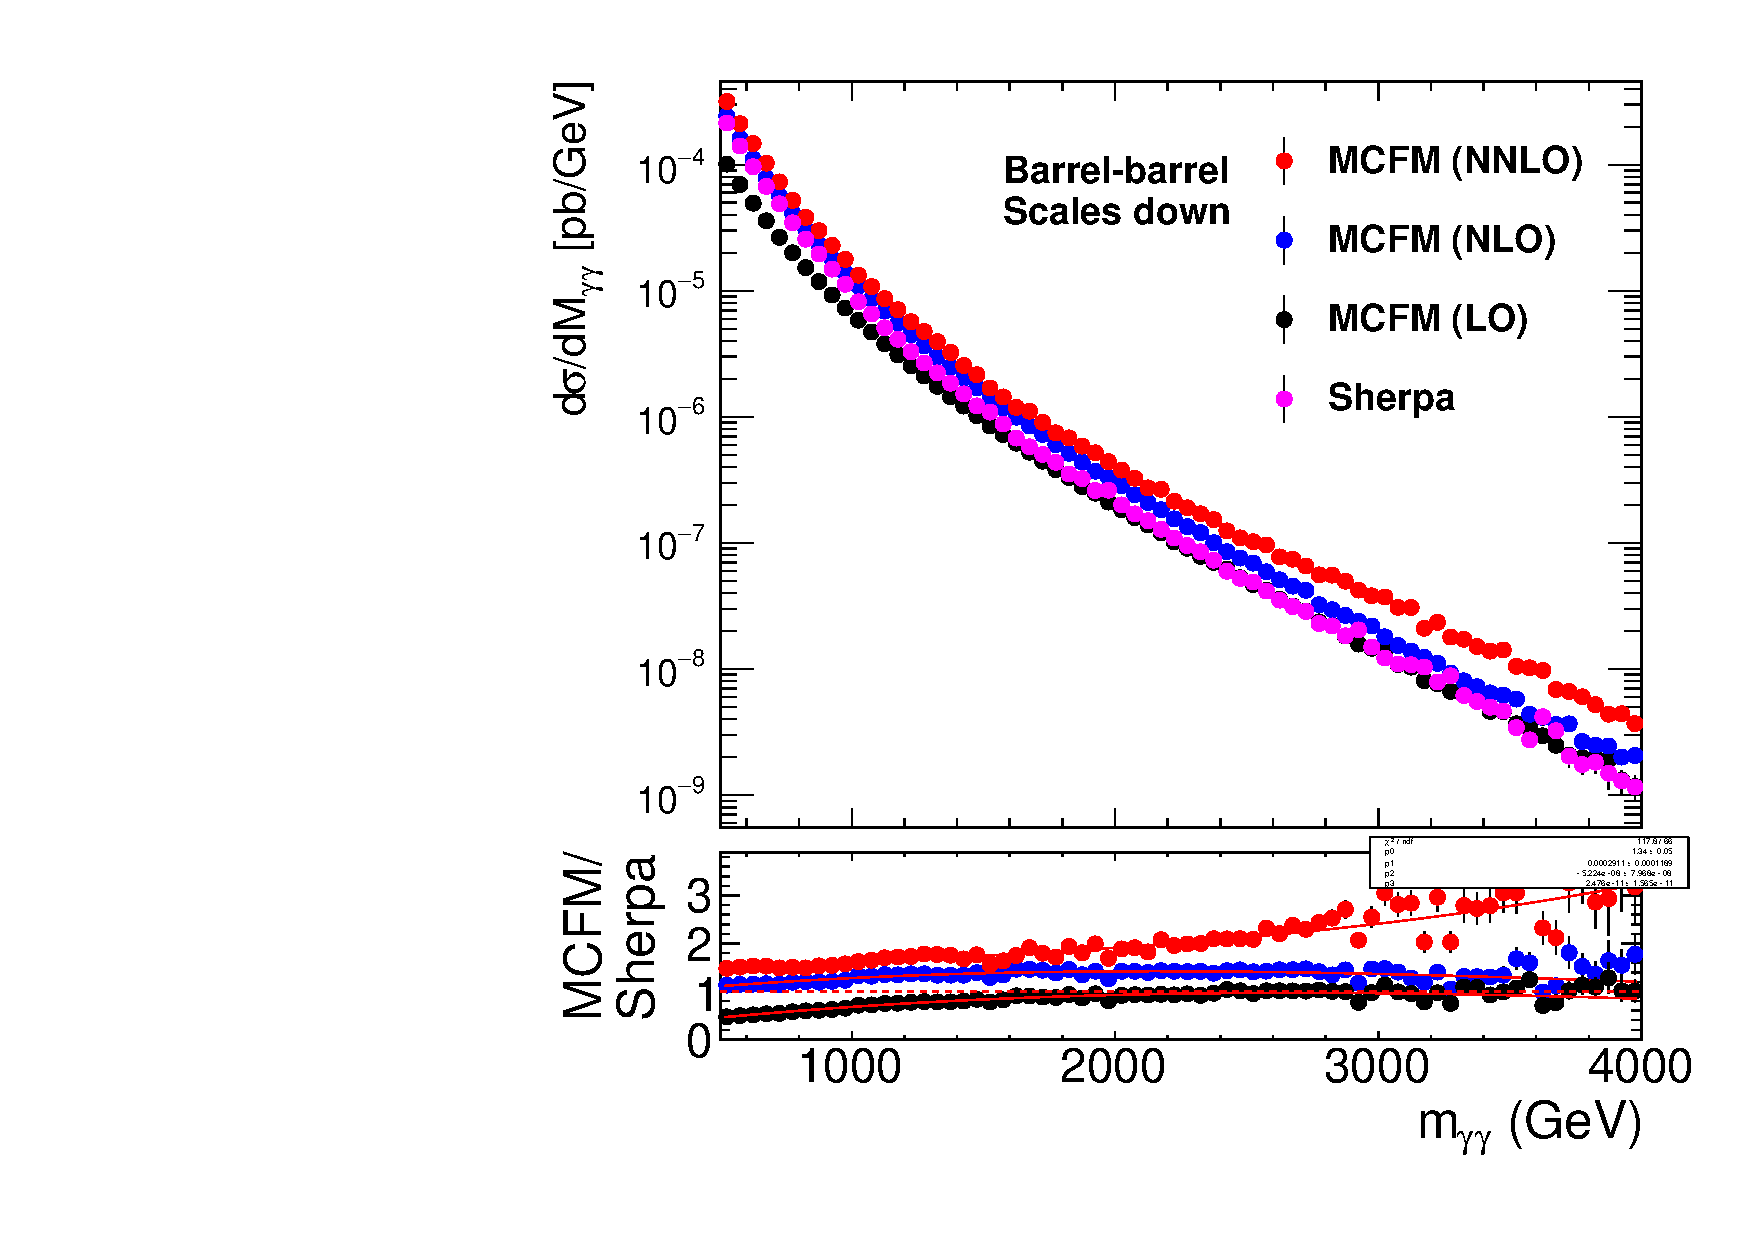
\includegraphics[angle=0,width=0.40\textwidth]{figures/BB_hist1_R0p5F0p5.pdf}
  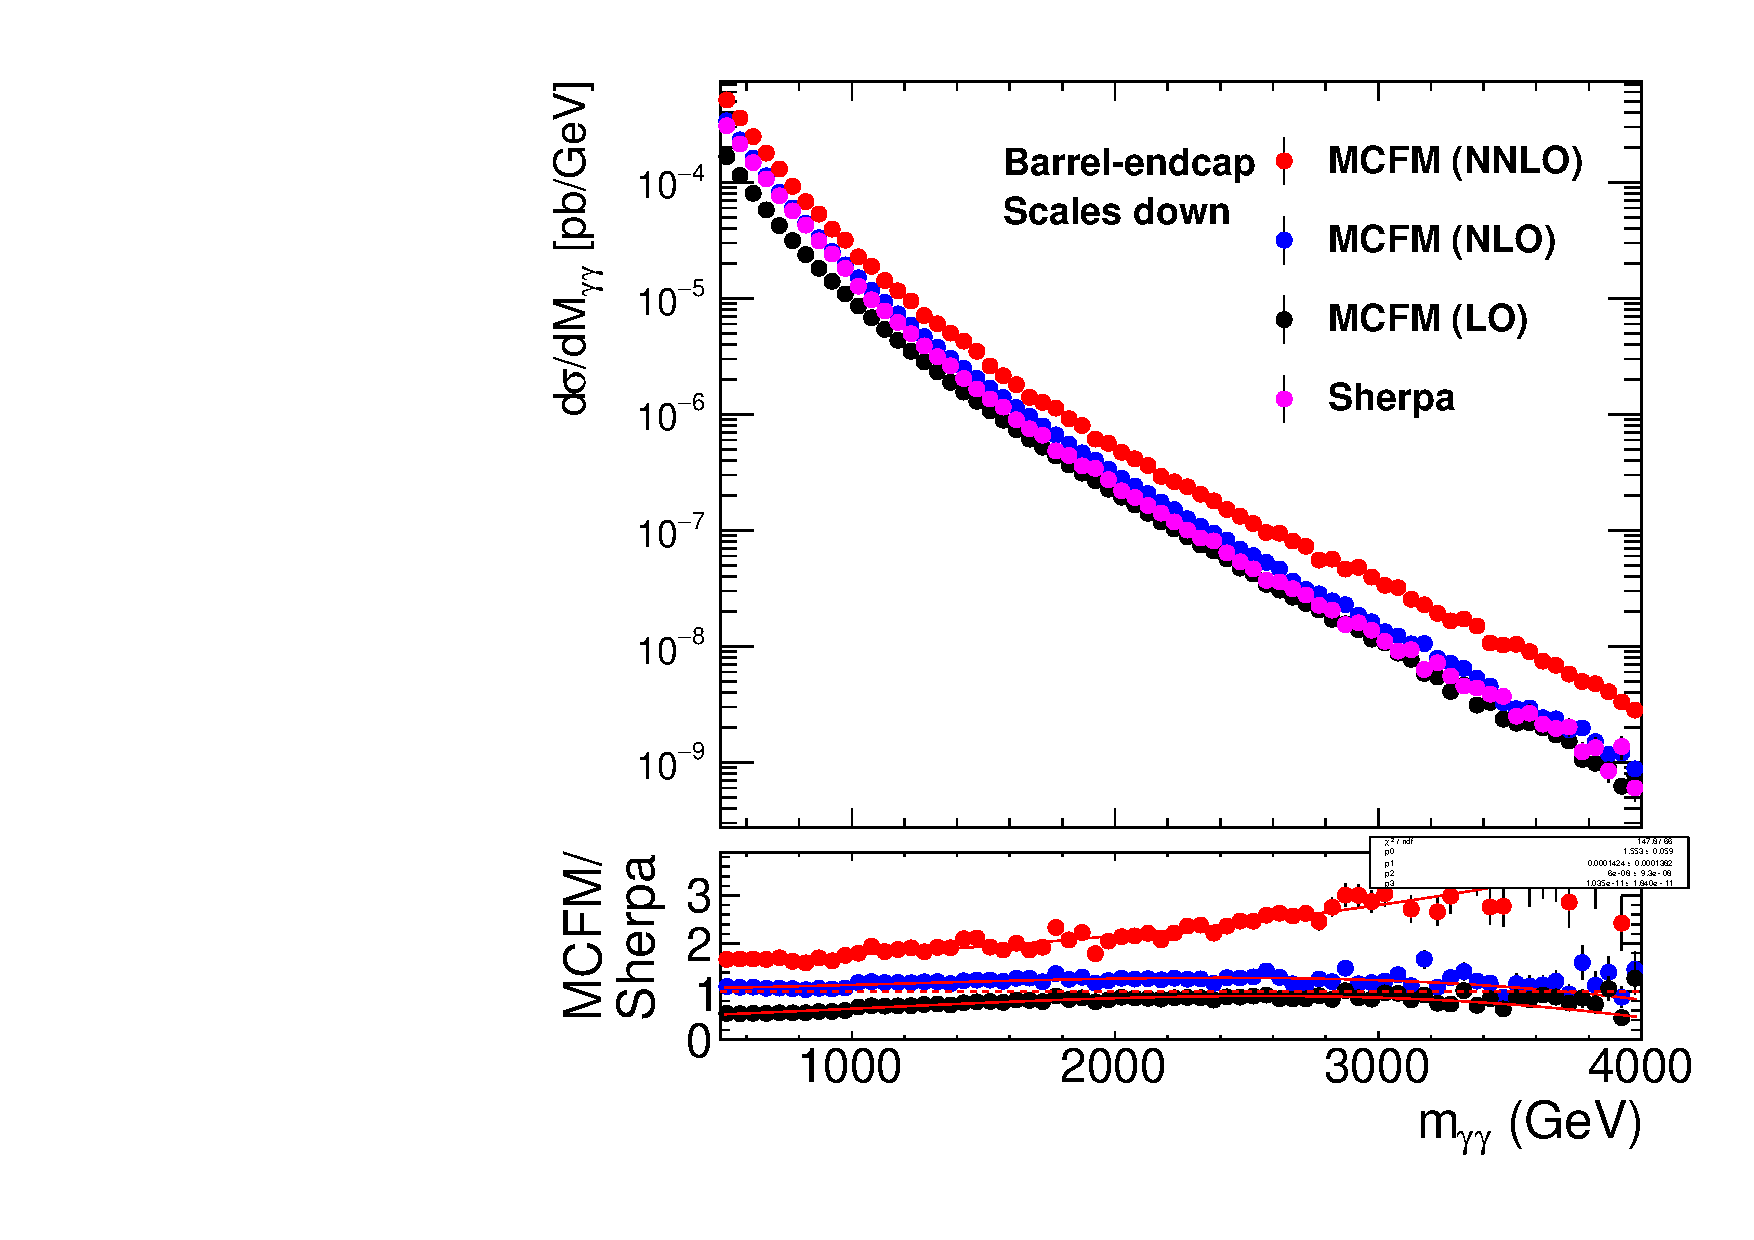
\includegraphics[angle=0,width=0.40\textwidth]{figures/BE_hist1_R0p5F0p5.pdf}
  \caption{The NNLO \Kfactor as a function of \Mgg in the EBEB (left) and EBEE (right) categories. The renormalization and factorization scales have been set to \mgg (middle) and simultaneously varied by factors of 2.0 (upper) and 0.5 (lower).}
  \label{fig:kfactor_mgg}
\end{figure}

\correction{Fig.~\ref{fig:kfactor_mgg} also shows the effects of simultaneously varying the renormalization $\mu_r$ and factorization $\mu_f$ scales by a factor of two up (upper) and down (lower) around the nominal prediction (center). The standard convention is to set these scales equal to each other and simultaneously vary them according to:}
\begin{itemize}
  \item $\mu_r = \mu_f = 2.0\Mgg$;
  \item $\mu_r = \mu_f = 1.0\Mgg$; and
  \item $\mu_r = \mu_f = 0.5\Mgg$.
\end{itemize}
\correction{\noindent These separate variations in the EBEB region are summarized for each order in Fig.~\ref{fig:kfactor_comparison_all}, which shows an envelope around the nominal \Kfactor prediction with these scales set to $1.0\Mgg$. This effect is treated as a systematic uncertainty on the analysis and is discussed in Chapter~\ref{ch:systematics}. Note, by default in \MCFM, the fragmentation scale is set to the renormalization scale. The fragmentation scale is the scale of the fragmentation functions, which describe the probability for a parton to fragment into a hadron. The variation of the renormalization scale indirectly varies this scale as well; however, its contribution is negligible when using Frixione isolation.}

\begin{figure}[htbp!]
  \centering
  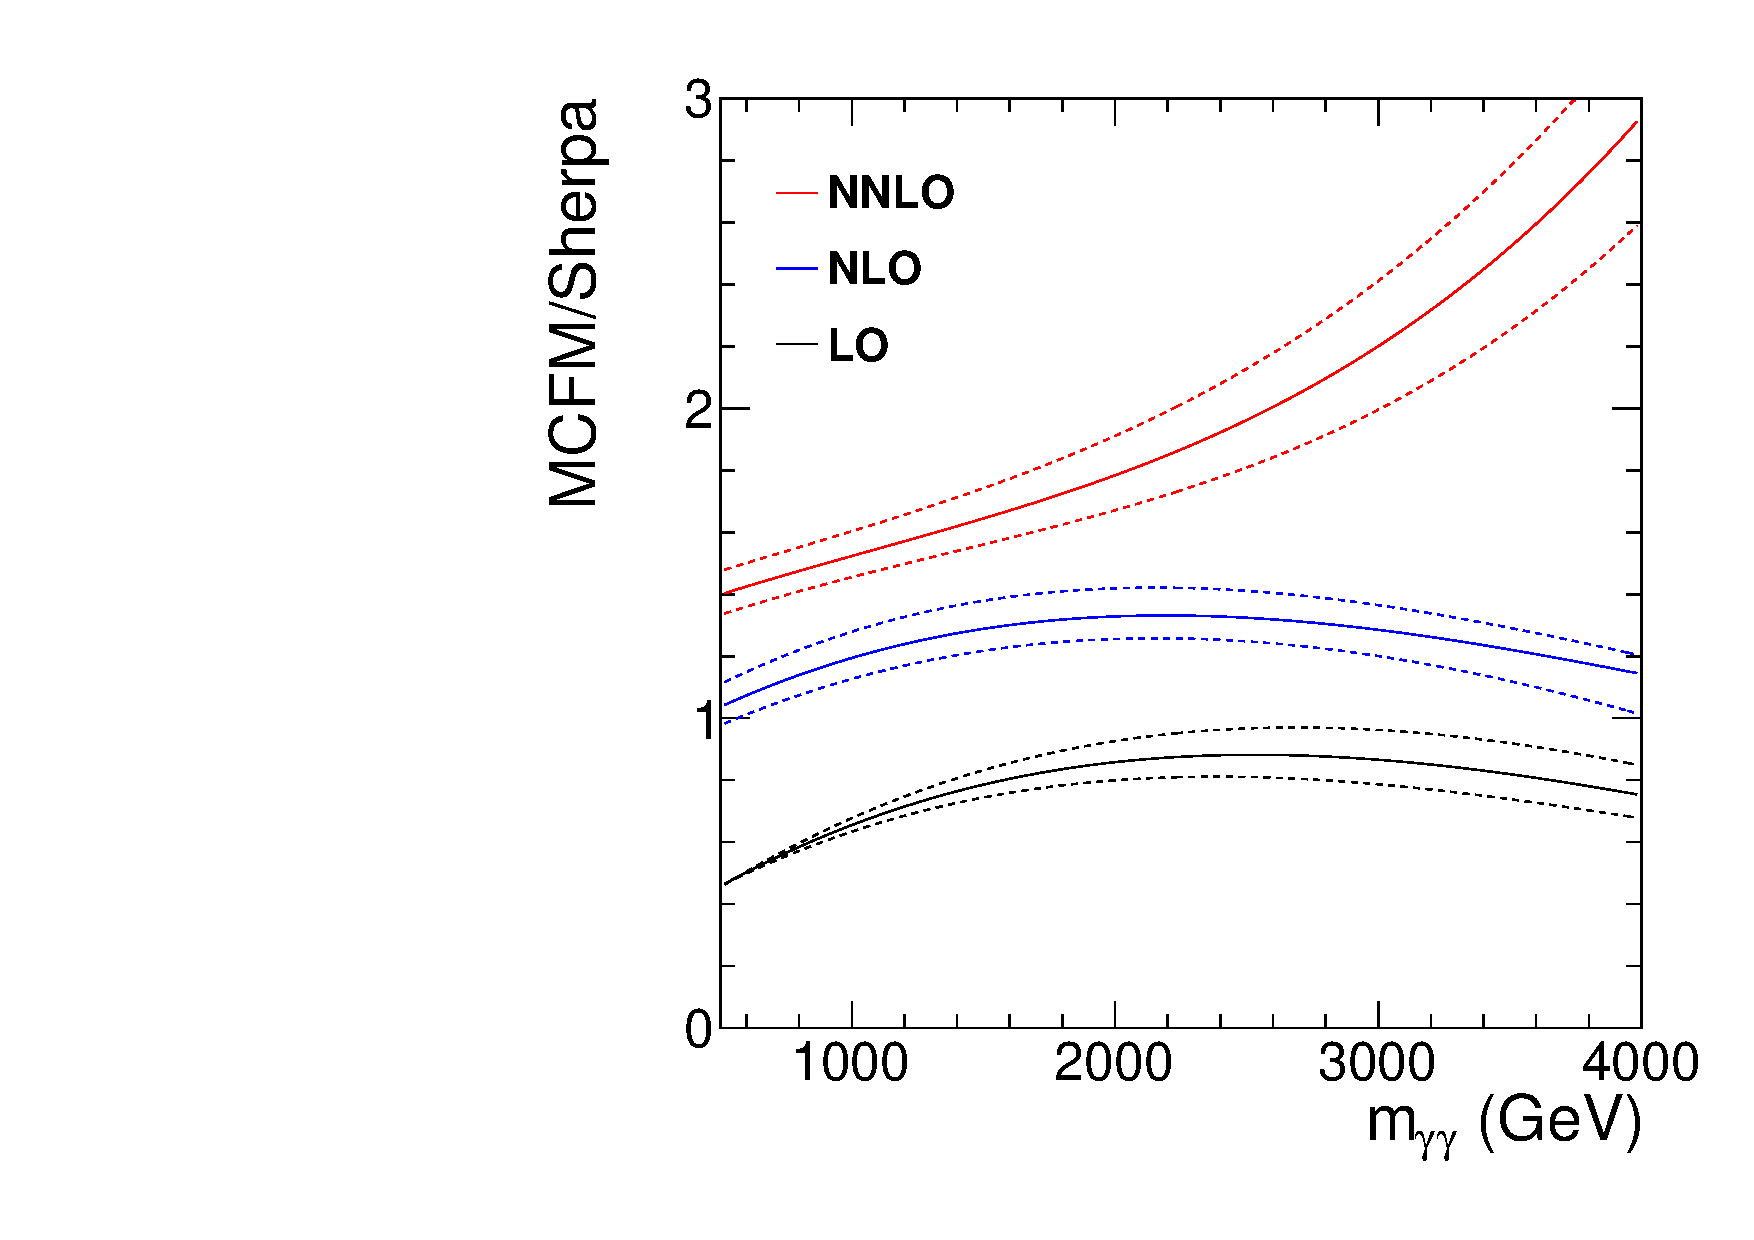
\includegraphics[angle=0,width=0.65\textwidth]{figures/kfactor_comparison.pdf}
  \caption{Ratio of the diphoton cross section calculated by \MCFM to that obtained from \SHERPA. The curves indicate different orders of the \MCFM calculation, and the dashed lines show the effect of the scale variations.}
  \label{fig:kfactor_comparison_all}
\end{figure}

\correction{The final prediction for the real SM diphoton background is determined by applying the \Kfactor to the fully simulated \SHERPA samples to reweight its events. The \Kfactor distributions are parameterized as a function of \Mgg, separately for the EBEB and EBEE categories, using a third degree polynomial function $f$ of the form}
\begin{equation}
  f(\Mgg) = p_0 + p_1\Mgg + p_2 \Mgg^2 + p_3 \Mgg^3
\end{equation}
\correction{\noindent where $p_i$, for $i=0$, 1, 2, and 3, are free parameters determined by a best fit to each distribution. The values of $p_i$ are shown in Table~\ref{tab:kfactor_values}, separately for each region. These functions are applied to the simulation-level \SHERPA events, yielding a full NNLO prediction of the real SM diphoton background.}

\begin{table}[hbt!]
  \caption{Parameters of the \Kfactor function for the EBEB and EBEE categories.}
  \label{tab:kfactor_values}
  \centering
  \vspace{\baselineskip}
  \begin{tabular}{r|rr}
    \hline
    \hline
          & EBEB & EBEE \\
    \hline
    $p_0$ & \correction{$1.25\pm0.04$} & \correction{$1.43\pm0.05$} \\
    $p_1$ & \correction{$3.36\mathrm{e}{\text{-}04}\pm1.05\mathrm{e}{\text{-}04}$} & \correction{$2.02\mathrm{e}{\text{-}04}\pm1.19\mathrm{e}{\text{-}04}$} \\
    $p_2$ & \correction{$-9.09\mathrm{e}{\text{-}08}\pm7.01\mathrm{e}{\text{-}08}$} & \correction{$-4.44\mathrm{e}{\text{-}09}\pm7.99\mathrm{e}{\text{-}08}$} \\
    $p_3$ & \correction{$2.82\mathrm{e}{\text{-}11}\pm1.38\mathrm{e}{\text{-}11}$} & \correction{$1.76\mathrm{e}{\text{-}11}\pm1.59\mathrm{e}{\text{-}11}$} \\
    \hline
    \hline
  \end{tabular}
\end{table}


\section{Background from Diphoton Misidentifications}\label{sec:fake_background}

A subdominant contribution to the total background in this search occurs when particles are misidentified as photons in the CMS detector. These particles fake a photon signature and are misreconstructed as photons. The background arising from this is referred to as the fake background. In this analysis, we consider fake photons arising from the misreconstruction of both electrons and jets. The rate for electrons faking photons is almost negligible and is readily measured from an MC calculation. To measure the rate for jets faking photons, a sophisticated technique using control samples in data is utilized.

The subdominant contribution to the fake background occurs when one or two electrons are misidentified as a photon in the detector. This mainly occurs when the electron track is misreconstructed or an electron converts late in the tracker leaving behind missing hits. This is measured using the MC simulation of Drell-Yan dielectron, $W\gamma$, $Z\gamma$, $W$, and $t\bar{t}\gamma$ events. The measurement is done by inverting the electron veto in the high-\pt photon ID and counting how many events pass this modified ID. The contribution of these fakes to the total background is calculated to be less than 1\%.

The dominant contribution to the fake background occurs when a jet with large electromagnetic activity is misidentified as a photon in the CMS detector, allowing it to pass the high-\pt photon ID criteria and, hence, fake a photon signature. The typical example of this occurs when a jet fragments to a boosted neutral meson, such as a $\pi^0$ or $\eta$, which then decays at high momentum to two photons. Both of these photons can then deposit their energy in the ECAL in such a way that their deposits overlap and resemble the signature of a single photon candidate. The fact that two photon energy deposits can become indistinguishable from one is due to the finite granularity and energy resolution of the ECAL. In a single diphoton event, this can occur from either one or two jets resulting in a photon\texttt{+}jet ($\gamma$j) or dijet (jj) background event, respectively. This type of jet fragmentation process is rare, so instead of relying on the MC simulation to accurately calculate it, a data-driven approach is preferred, which uses control samples in data to estimate to estimate the fake background contribution. The approach utilized is referred to as the fake rate method.


\subsection{Fake Rate Method}

The fake rate method involves determining a fake rate $f$ from a jet-enriched data control sample and applying it to the analysis dataset containing diphotons passing the final analysis selection. The fake rate is defined as the ratio of the number of jets passing two categories of jet fragmentation processes. The first category, the numerator of the ratio, is the number of jets passing the high-\pt photon ID. The second category, the denominator of the ratio, is the number of jets passing a looser, photon-like ID. The denominator ID is chosen such that the two categories are orthogonal. In equation form, the fake rate is
\begin{equation}
  f = \frac{(\text{numerator})}{(\text{denominator})} = \frac{\# \left\lbrace\text{jets passing the photon ID}\right\rbrace}{\# \left\lbrace\text{jets passing a photon-like ID}\right\rbrace}
\end{equation}
\noindent where \# is used to denote the number of objects in that category. This fake rate $f$ is simply the ratio of its defined categories and is not the probability that a generic jet will fake a photon.

A complication arises when determining the numerator. Although the control data sample is jet enriched, there will inevitability be a contribution to the numerator from genuine photons in it passing the photon ID, which must be removed. This is done through a fitting procedure where template models of real and fake photons are fit to the data in the control sample. These templates are constructed using a photon ID variable that is sensitive to the differences between real and fake photons, such as a shower shape or isolation variable. After the fit is performed, the contribution to the numerator from real photons will be subtracted from the total. In general, the choice of template variable will evolve with photon \pt and $\eta$. Therefore, the fake rate $f$ will be measured as a function of photon \pt and categorized in the EB and EE regions.

After the final fake rate function $f(\pt)$ is determined separately in the EB and EE categories (from the data control sample), it will then be applied to the final, analysis-level diphoton dataset. This is done by selecting objects in the diphoton dataset that pass the denominator, photon-like ID and reweighting them using $f(\pt)$, separately in the EBEB and EBEE categories. The assumption in doing this final step is that taking denominator objects and reweighting them by the fake rate does indeed produce an accurate representation of the kinematics of known fake events. Physically, we expect this to be true because jet fragmentation is largely independent of the rest of the event. \correction{Thus, events where a jet fragments to look like a denominator, photon-like jet should be representative of other events where the jet fragmented differently and ended up faking the photon ID, since we want to measure the number of jets passing the photon ID by using jets that pass the denominator ID.} Verification of the ability of the fake rate method to achieve this is demonstrated in simulation and is described in Section~\ref{sec:closure_test_kinematics}.

\correction{To validate the fake rate method, a closure test is performed on a sample of simulated data produced from an MC calculation.} The idea is to apply the fake rate method to the simulated sample in the identical way as it is done in the jet-enriched control dataset. This yields a fake prediction in the simulated sample. Now, because we are using simulation, we have access to the MC truth information for the particles, i.e., we know the properties and full event history of all the particles in the simulated sample. In particular, we know the identities of all of the particles in it passing the high-\pt photon ID. Therefore, using the truth information, we can tag objects passing the photon ID as having arisen from jets or from real, prompt photons. Finally, we can compare these fake yields to the fake prediction in the simulated sample. In addition, we also perform further studies to validate the method, as will be explored in Section~\ref{ssec:closure_test}.


\subsection{Fake Rate Calculation}

The data control sample used for the photon fake rate calculation comes from a combination of jet- and muon-triggered data samples. The list of samples using the full, internal CMS dataset path names are tabulated in Table~\ref{tab:fake_rate_datasets}. This combination of datasets has been constructed to help eliminate any potential bias arising from the differences in the hadronization between quarks and gluons. In general, gluon jets contain a higher number of particles, as discussed in Section~\ref{sec:jets}, and are therefore less likely to pass the isolation variables in the photon ID, so they should have a lower probability of faking a photon than a quark jet. It is difficult to distinguish between quark and gluon jets in data, but these datasets result from different processes and will help better sample jet flavor in the control sample.

\begin{table}[!htbp]
  \caption{Control datasets used for the photon fake rate calculation.}
  \label{tab:fake_rate_datasets}
  \centering
  \vspace{\baselineskip}
  \small %\normalsize %\footnotesize
  \begin{tabular}{l}
  \hline
  \hline
  Dataset path \\
  \hline
  /JetHT/Run2016B-23Sep2016-v3/MINIAOD \\
  /JetHT/Run2016C-23Sep2016-v1/MINIAOD \\
  /JetHT/Run2016D-23Sep2016-v1/MINIAOD \\
  /JetHT/Run2016E-23Sep2016-v1/MINIAOD \\
  /JetHT/Run2016F-23Sep2016-v1/MINIAOD \\
  /JetHT/Run2016G-23Sep2016-v1/MINIAOD \\
  /JetHT/Run2016H-PromptReco-v2/MINIAOD \\
  /JetHT/Run2016H-PromptReco-v3/MINIAOD \\
  \hline
  /DoubleMuon/Run2016B-23Sep2016-v3/MINIAOD \\
  /DoubleMuon/Run2016C-23Sep2016-v1/MINIAOD \\
  /DoubleMuon/Run2016D-23Sep2016-v1/MINIAOD \\
  /DoubleMuon/Run2016E-23Sep2016-v1/MINIAOD \\
  /DoubleMuon/Run2016F-23Sep2016-v1/MINIAOD \\
  /DoubleMuon/Run2016G-23Sep2016-v1/MINIAOD \\
  /DoubleMuon/Run2016H-PromptReco-v2/MINIAOD \\
  /DoubleMuon/Run2016H-PromptReco-v3/MINIAOD \\
  \hline
  \hline
  \end{tabular}
\end{table}

As the proton beams circulate, they may interact with the LHC collimators or residual gas in the beam pipe due to the non-perfect vacuum, creating ``beam halo." When the protons interact with the particles associated with these sources, jets will be formed and can subsequently fragment to other high-energy particles, which are not produced from the collision point of the bunch crossing. This will produce charged pions ($\pi^{\pm}$), which will travel an average distance of about 10~m before decaying, primarily to muons ($\mu^{\pm}$). These muons will travel parallel to the beam pipe and can traverse the whole detector, producing high-energy bremsstrahlung photons in the ECAL. Beam halo could fake a photon signature and must be eliminated in the fake rate measurement. This \correction{source can be identified and rejected} by using the photon shower shape variables \sieie and \sipip. Beam halo will be well contained in the $\phi$ direction but spread out in the $\eta$ direction as it interacts with the CMS detector. This is in contrast to prompt photons, which are well contained in the $\eta$ direction. Fig.~\ref{fig:sipip_vs_sieie} shows the correlation between \sieie and \sipip for all objects in the jet-triggered dataset passing the high-\pt photon ID (with the \sieie cut relaxed) in the range $450<\pt<500\GeV$. In this high-energy range, cutting at $\sipip > 0.009$ will safely reject the beam halo.

\begin{figure}[!htbp]
  \centering
  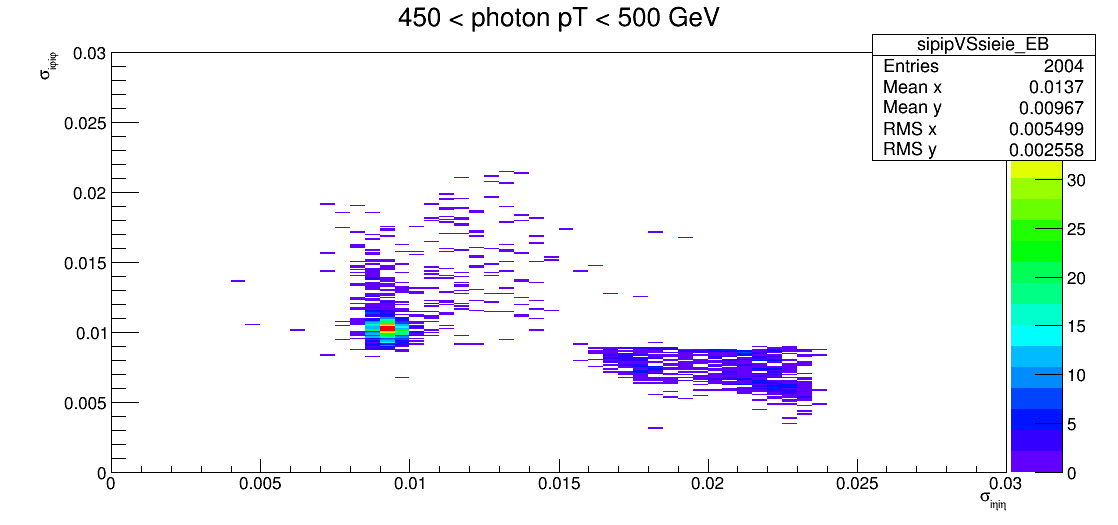
\includegraphics[scale=0.43]{figures/sipip_vs_sieie_EB_pT450-500.png}
  \caption{The correlation between \sieie and \sipip for all objects in the jet-triggered control dataset (used for the fake rate calculation) passing the high-\pt photon ID (with the \sieie cut relaxed) in the range $450<\pt<500\GeV$. Beam halo is observed for $\sipip < 0.009$.}
  \label{fig:sipip_vs_sieie}
\end{figure}

The denominator objects are chosen to pass a less strict version of the high-\pt photon ID. These photon-like jets should have high electromagnetic energy content but are required to fail at least one of the photon ID variables, ensuring the denominator category is orthogonal to the numerator category, as well as eliminating any contamination from real photons. We want these objects to be representative of the kinematics of the reweighted events in the diphoton data sample. They should be reasonably isolated since not all of the energy of the particles in a cone of $\Delta R$ around the object is added to it, while, on the other hand, \correction{we need to ensure there is enough statistics} after loosening the isolation criteria. Different cuts are imposed in the EB and EE regions to optimize the selection in each category. Denominator objects in the EB are required to fail at least one of the variables \hoe, \sieie, \chiso, or \corphoiso. In addition, they are required to pass both $\chiso < 0.2\,\pt$ and $\corphoiso < 0.2\,\pt$. Because of pileup mismodeling in the $\phoiso$ variable during the 2016 data-taking period, denominator objects in the EE category are required to pass the photon ID cut of $\corphoiso < 2.0\GeV$, instead of the looser selection of $\corphoiso < 0.2\,\pt$. In the EE regions, the denominator objects are also required to pass $\chiso < 0.2\,\pt$ and fail at least one of the variables \hoe, \sieie, or \chiso. These cuts will be summarized in Table~\ref{tab:fake_rate_cuts} below after some further discussion.

An additional cut for denominator objects on the ratio the hadronic over electromagnetic energies using $\text{Hadronic/E}$ is imposed in both the EB and EE regions. As discussed in Section~\ref{sec:trigger}, the variable \hoe using a tower-based isolation to sum the hadronic energy deposits while $\text{Hadronic/E}$ uses a cone-based calculation. The trigger selection used in the analysis (\texttt{HLT\_DoublePhoton60}) requires $\text{Hadronic/E}$ at the HLT level and is not fully efficient for denominator objects, even for those passing $\hoe < 0.05$, while it is for objects passing the high-\pt photon ID. This is remedied by applying an additional cut of $\text{Hadronic/E} < 0.1$ to the denominator objects.

The numerator objects result from the selection of objects in the jet-enriched dataset passing the high-\pt photon ID and adjusted so that any contamination from real photons is removed through a template fitting procedure. The template variable used is the shower shape variable \sieie. The data to be fit to are the numerator candidates in the jet-enriched dataset consisting of all objects passing the high-\pt photon ID with \sieie relaxed, to be summarized in Table~\ref{tab:fake_rate_cuts} below. Since \sieie evolves with photon \pt, the data are divided into the nine photon \pt bins of 50-70, 70-90, 90-110, 110-130, 130-150, 150-200, 200-250, 250-300, and 300-600\GeV. (The denominator objects are also split into these bins resulting in a fake rate for each bin.) The numerator candidates in each \pt bin are split into their real and fake components using templates derived from respective models of real and fake photons.

The fake templates are derived from the jet-enriched dataset. Since real photons are well isolated after pileup subtraction, in particular, the high-\pt photon ID requires $\chiso < 5\GeV$, fake photons can be modeled by inverting this isolation requirement. Objects in the fake templates must pass the high-\pt photon ID with \sieie relaxed but are taken from the sideband of $5 < \chiso < 10\GeV$. Notice, we are trying to describe fake photons with $\chiso < 5\GeV$ by modeling them from the selection using $5 < \chiso < 10\GeV$. The evolution of the fake templates with \pt from the jet-triggered dataset is shown in Fig.~\ref{fig:fake_templates}. These templates are scaled to 1\fbinv and shown separately in the EB and EE regions.

\begin{figure}[!htbp]
  \centering
  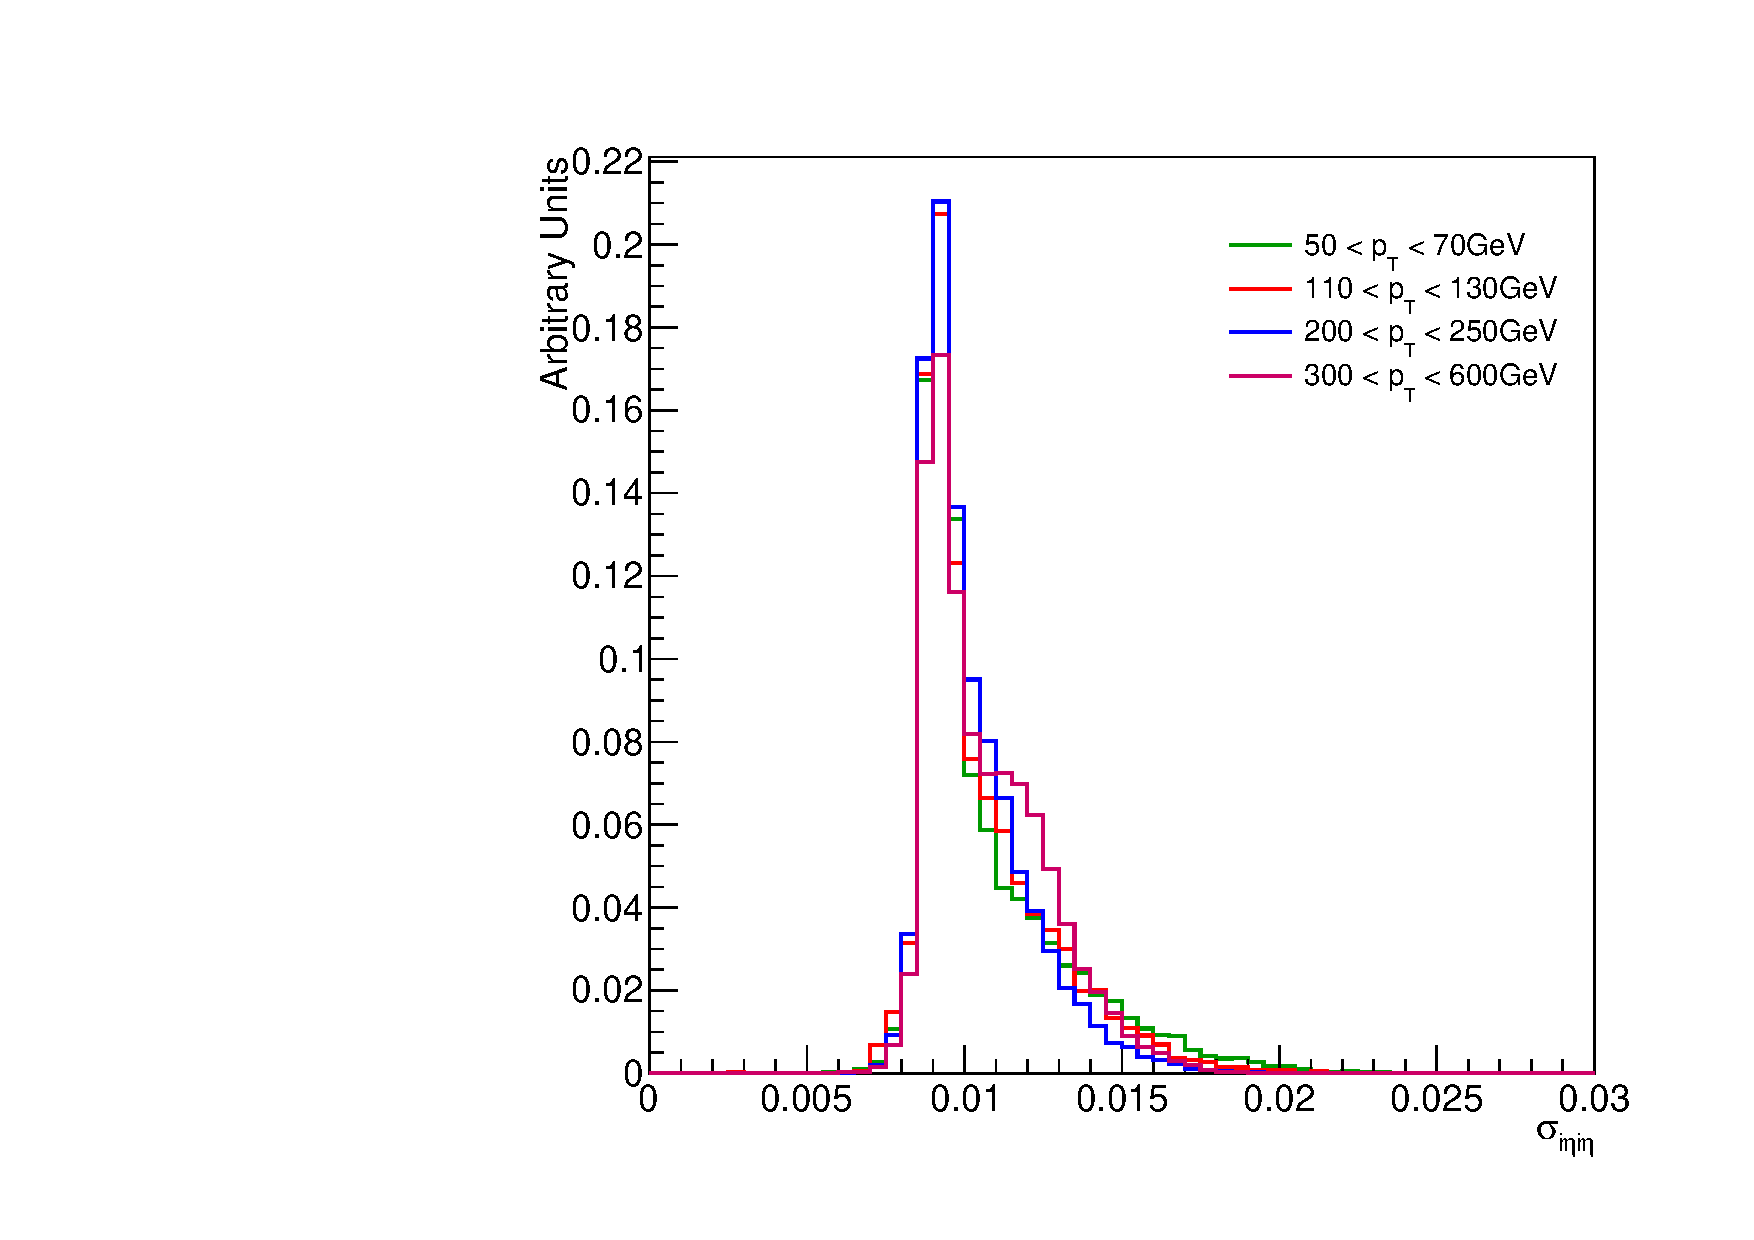
\includegraphics[width=0.45\textwidth]{figures/faketemplatecompEB.pdf}
  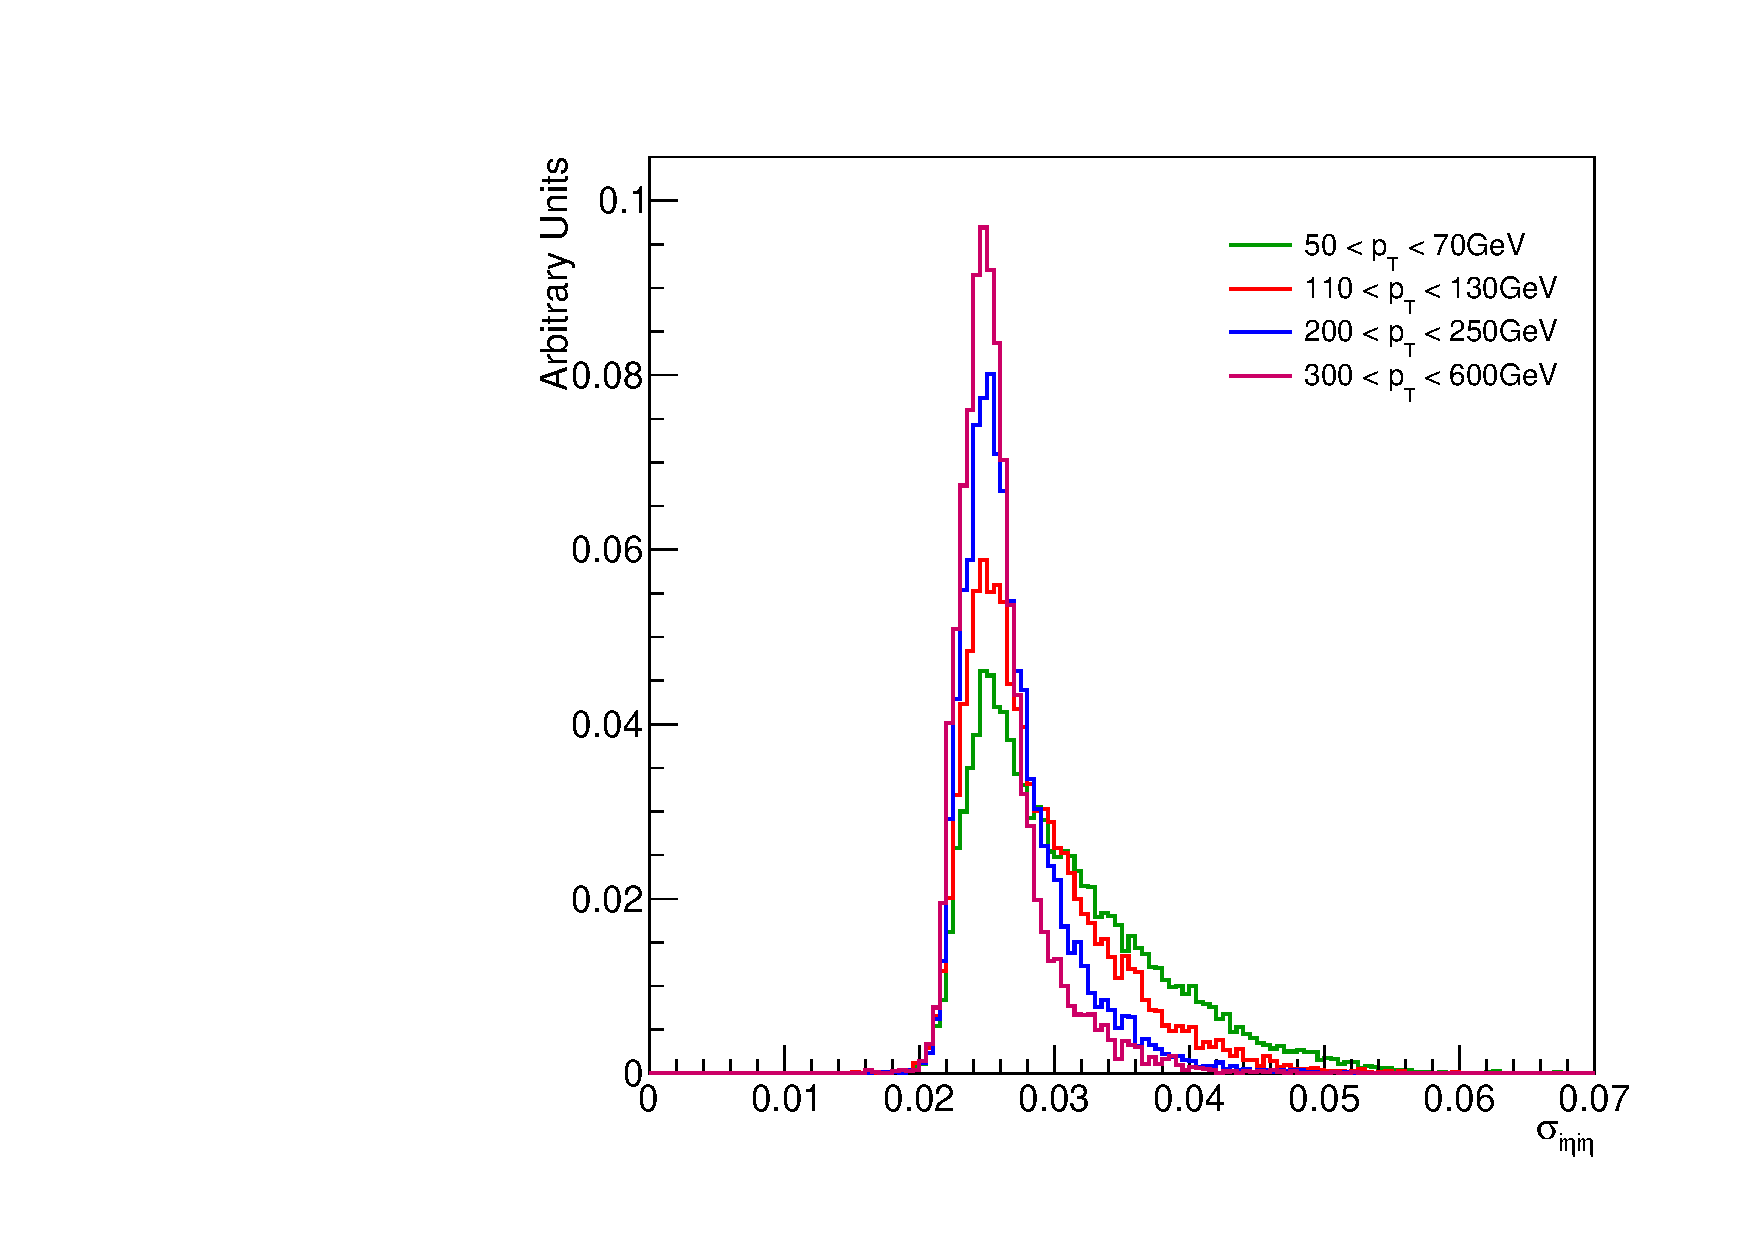
\includegraphics[width=0.45\textwidth]{figures/faketemplatecompEE.pdf}
  \caption{Fake templates scaled to 1\fbinv in various \pt bins in the EB (left) and EE (right) regions.}
  \label{fig:fake_templates}
\end{figure}

The real templates are derived from a photon-rich simulated sample produced using an MC calculation. The $\gamma\gamma$ MC background samples, listed in Table~\ref{tab:ggjets_samples}, are used for this. In addition, the $\gamma$j MC samples produced centrally within the CMS Collaboration are added to allow for a source of prompt photons coming from processes using the $\gamma$j final state. The full list of samples is given in Table~\ref{tab:real_template_samples}. Within the photon-rich MC sample, all objects passing the high-\pt photon ID with relaxed \sieie are selected, but only those coming from known prompt photons are allowed in the real templates. The definitions for both the real and fake templates are summarized in Table~\ref{tab:fake_rate_cuts}. It's possible to identify these real photons since the MC truth information is provided for all generated particles.

\begin{table}[!htbp]
  \caption{The MC samples and corresponding cross sections used for deriving the real templates in the fake rate calculation. The full, internal CMS path name is specified by appending the dataset path with \texttt{/RunIISummer16MiniAODv2-\allowbreak PUMoriond17\_\allowbreak 80X\_\allowbreak mcRun2\_\allowbreak asymptotic\_\allowbreak 2016\_\allowbreak TrancheIV\_\allowbreak v6/\allowbreak MINIAODSIM}.}
  \label{tab:real_template_samples}
  \centering
  \vspace{\baselineskip}
  %\footnotesize
  \small
  \begin{tabular}{lc}
  \hline
  \hline
  Dataset path & Cross section (pb) \\ 
  \hline
  /GGJets\_M-60To200\_Pt-50\_13TeV-sherpa & 5.785 \\
  /GGJets\_M-200To500\_Pt-50\_13TeV-sherpa & 2.244 \\
  /GGJets\_M-500To1000\_Pt-50\_13TeV-sherpa & 1.510 \\
  /GGJets\_M-1000To2000\_Pt-50\_13TeV-sherpa & 1.084e-02 \\
  /GGJets\_M-2000To4000\_Pt-50\_13TeV-sherpa & 3.690e-04 \\
  /GGJets\_M-4000To6000\_Pt-50\_13TeV-sherpa & 2.451e-06 \\
  /GGJets\_M-6000To8000\_Pt-50\_13TeV-sherpa & 1.753e-08 \\
  /GGJets\_M-8000To13000\_Pt-50\_13TeV-sherpa & 7.053e-11 \\
  \hline
  /GJets\_HT-40To100\_TuneCUETP8M1\_13TeV-madgraphMLM-pythia8 & 2.121e+04 \\
  /GJets\_HT-100To200\_TuneCUETP8M1\_13TeV-madgraphMLM-pythia8 & 9.863e+03 \\
  /GJets\_HT-200To400\_TuneCUETP8M1\_13TeV-madgraphMLM-pythia8 & 2.298e+03 \\
  /GJets\_HT-400To600\_TuneCUETP8M1\_13TeV-madgraphMLM-pythia8 & 2.816e+02 \\ 
  /GJets\_HT-600ToInf\_TuneCUETP8M1\_13TeV-madgraphMLM-pythia8 & 9.465e+01 \\
  \hline \hline
  \end{tabular}
\end{table}

\begin{table}[!htbp]
  \caption{The cut-based definitions of the numerator and denominator objects for the fake rate calculation compared against the high-\pt photon ID. The numerator is determined after numerator candidates are fit with real and fake templates (definitions shown) using the template variable \sieie. The cuts listed are for both the EB and EE regions unless separately specified.}
  \label{tab:fake_rate_cuts}
  \centering
  \vspace{\baselineskip}
  \tiny
  \begin{tabular}{l|cccccc}
  \hline \hline
  Cut [EB \{sat.\} (EE \{sat.\})] & Photon ID & Num. & Real template & Fake template & Denom. (EB) & Denom. (EE) \\
  \hline
   & & & & & & \\
  \textbf{Photon ID cuts} & & & & & & \\
  \hline
  $\hoe < 0.05$ & pass & pass & pass & pass & \multirow{5}{*}{fail at least one} &  \multirow{4}{*}{fail at least one} \\
  $\sieie < 0.0105\, \{0.0112\}\, (0.028\, \{0.030\})$ & pass & template & template & template & & \\
  $\chiso < 5\GeV$ & pass & pass & pass & not applied & & \\
  $\corphoiso < 2.75\, (2.00)\GeV$ & pass & pass & pass & pass & & pass \\
  $\rnine > 0.8$ & pass & pass & pass & pass & pass & pass \\
   & & & & & & \\
  \textbf{Electron veto} & & & & & & \\
  \hline
  CSEV & pass & pass & pass & pass & pass & pass \\
   & & & & & & \\
  \textbf{Additional fake rate cuts} & & & & & & \\
  \hline
  $\sigma_{i\phi i\phi} > 0.009$ & not applied & pass & pass & pass & pass & pass \\
  $5 < \chiso < 10\GeV$ & not applied & not applied & not applied & pass & not applied & not applied \\
  $\text{Hadronic/E} < 0.1$ & not applied & not applied & not applied & not applied & pass & pass \\
  $\chiso < 0.2\,\pt$ & not applied & not applied & not applied & not applied & pass & pass \\
  $\corphoiso < 0.2\,\pt$ & not applied & not applied & not applied & not applied & pass & not applied \\
  \hline \hline
  \end{tabular}
\end{table}

The procedure used to ensure only real photons are selected is to first find the best match in $\Delta R$ among all the final state generated particles to the reconstructed photon object passing the photon ID. Next, the best match is required to be a generated photon within $\Delta R<0.1$. If the matched generated photon can be traced back to the hard interaction, then the reconstructed photon object is included in the real template. Fig.~\ref{fig:real_templates} shows the evolution of these real templates (each scaled to 1\fbinv) with photon \pt in both the EB and EE categories.

\begin{figure}[!htbp]
  \centering
  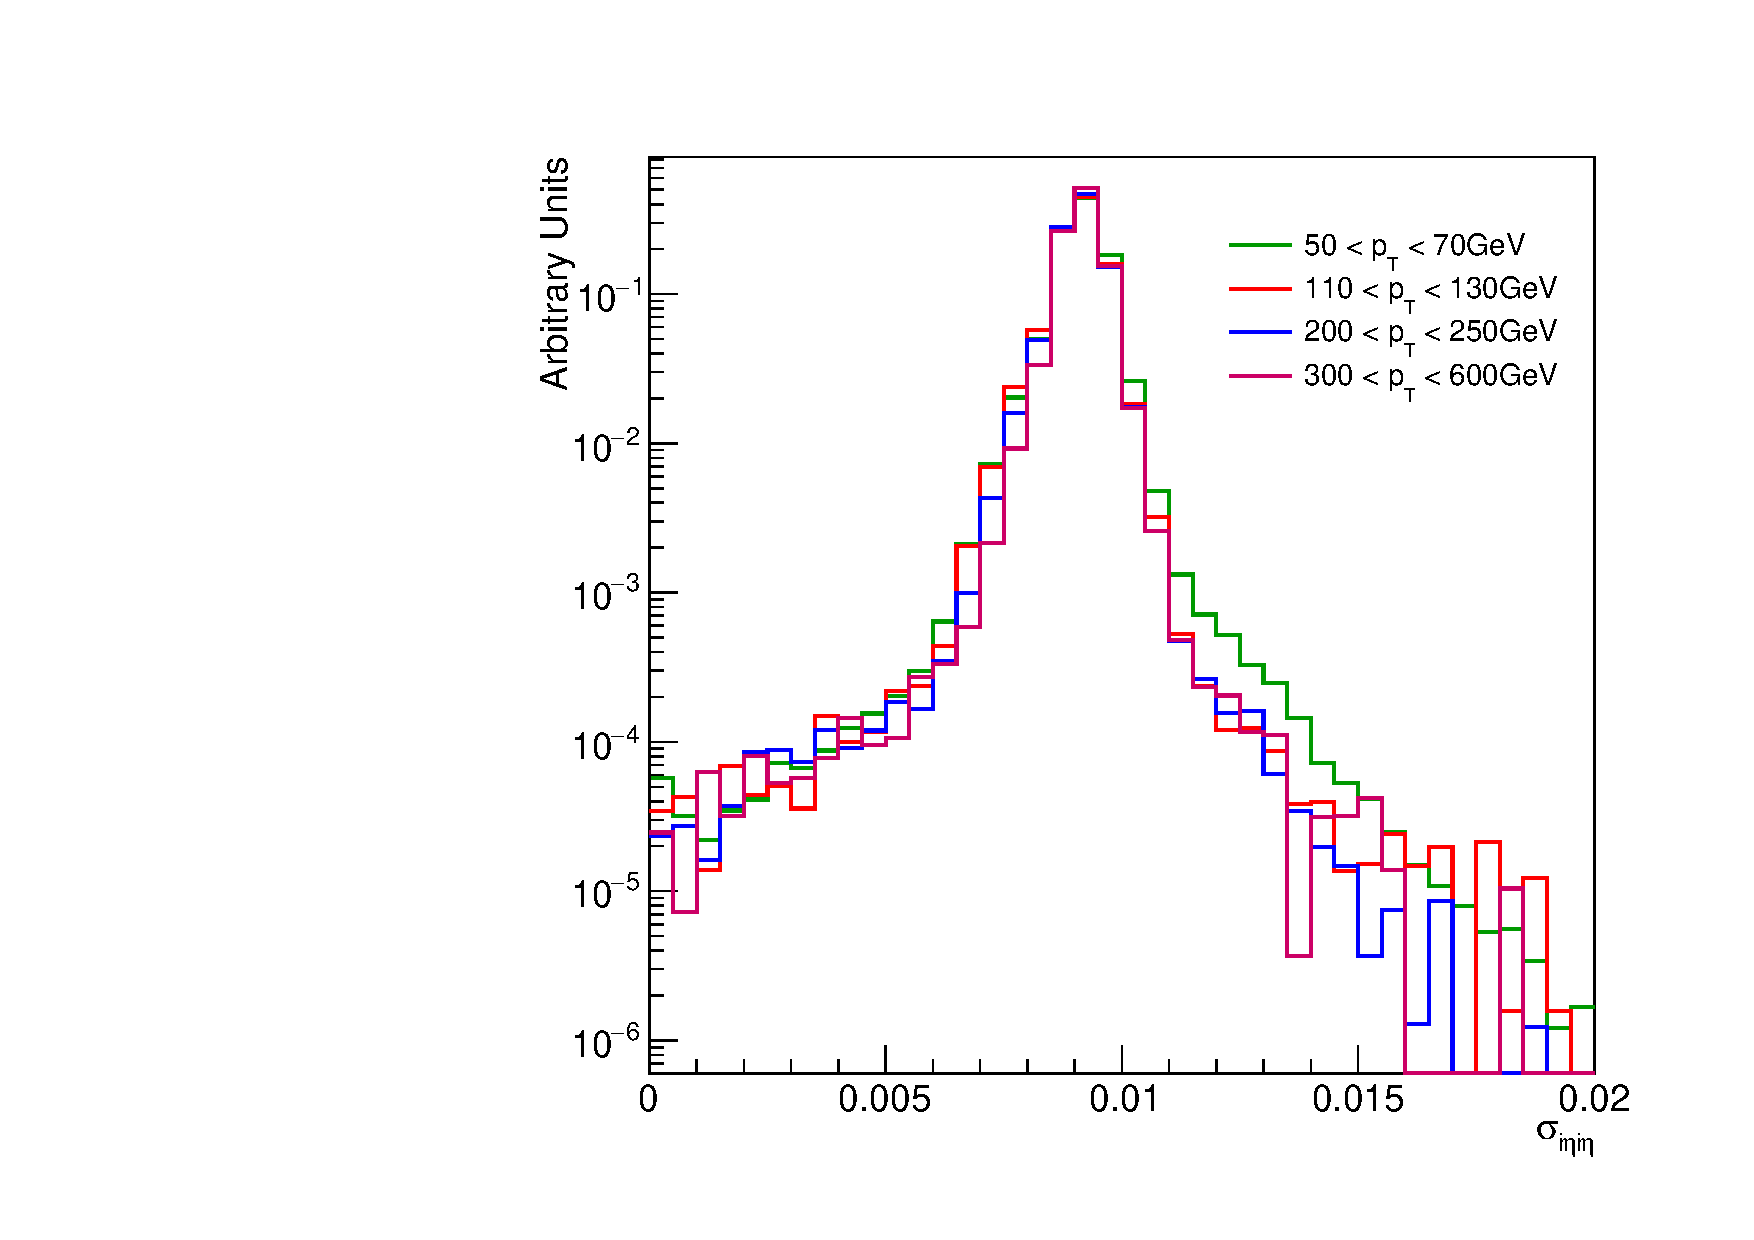
\includegraphics[width=0.45\textwidth]{figures/realtemplatecompEB.pdf}
  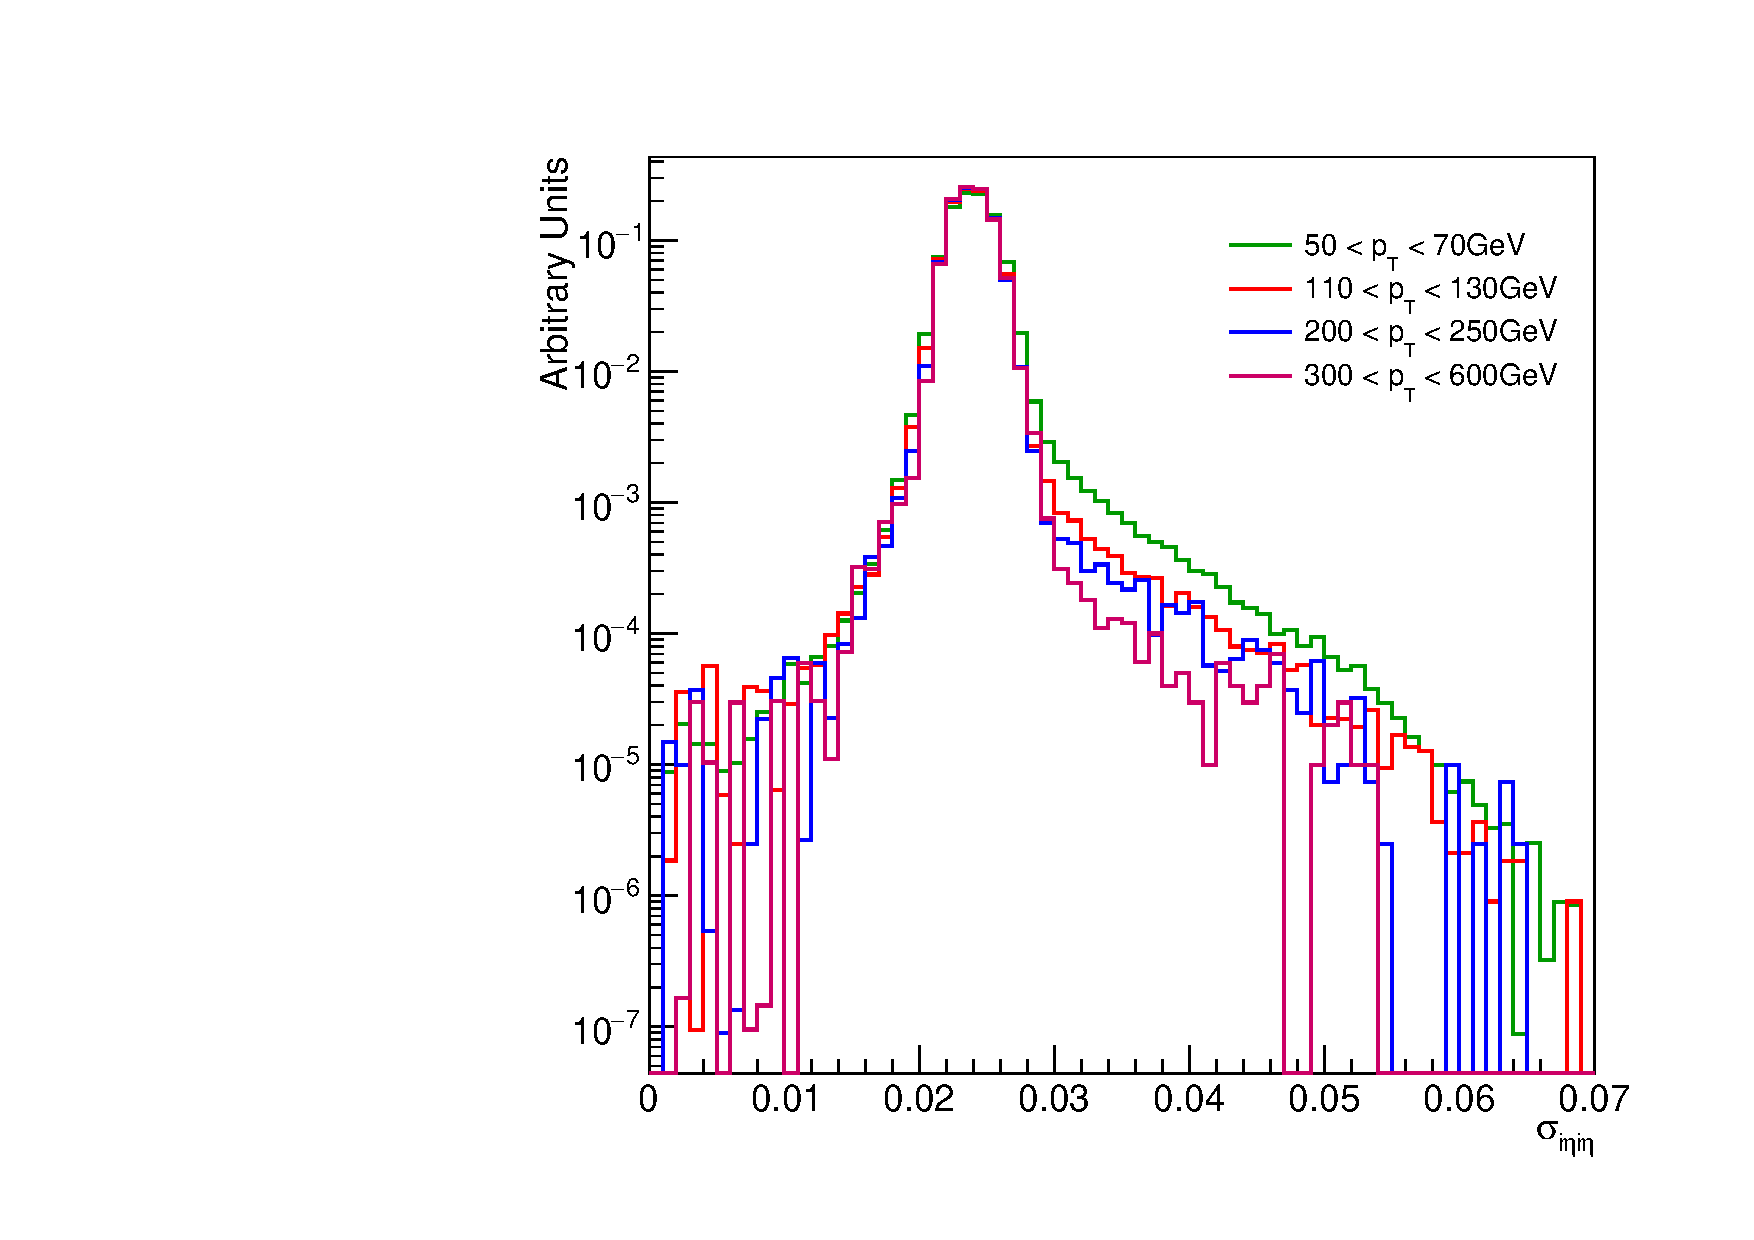
\includegraphics[width=0.45\textwidth]{figures/realtemplatecompEE.pdf}
  \caption{Real templates scaled to 1\fbinv in various photon \pt bins in the EB (left) and EE (right) regions.}
  \label{fig:real_templates}
\end{figure}

With the construction of the fake and real templates, they can both be fit to the numerator candidates in the control data sample. The shapes of the templates are fully determined from their construction, but their normalization is determined from the fit to the data. First the templates are normalized to $1\fbinv$, then a simultaneous fit using a maximum likelihood estimation is performed. A negative log-likelihood is used in a procedure similar to what is employed in Chapter~\ref{ch:results}. \correction{An example fit in the EB region for the 130-150\GeV \pt bin is shown in Fig.~\ref{fig:template_fit}. We see that the tail region with $\sieie > 0.011$ is dominated by fakes, which largely fixes the overall fake normalization.} The general trend showing that the real template dominates the overall normalization in the peak and the fake template in the tail holds true for the other \pt bins and also in the EE category. This final fit shows the contribution of fakes within the data. To extract the numerator, the fake template is integrated from 0 to \sieie cut value, which differs between the EB and EE categories. This process is repeated for all \pt bins in both categories.

\begin{figure}[!htbp]
  \centering
  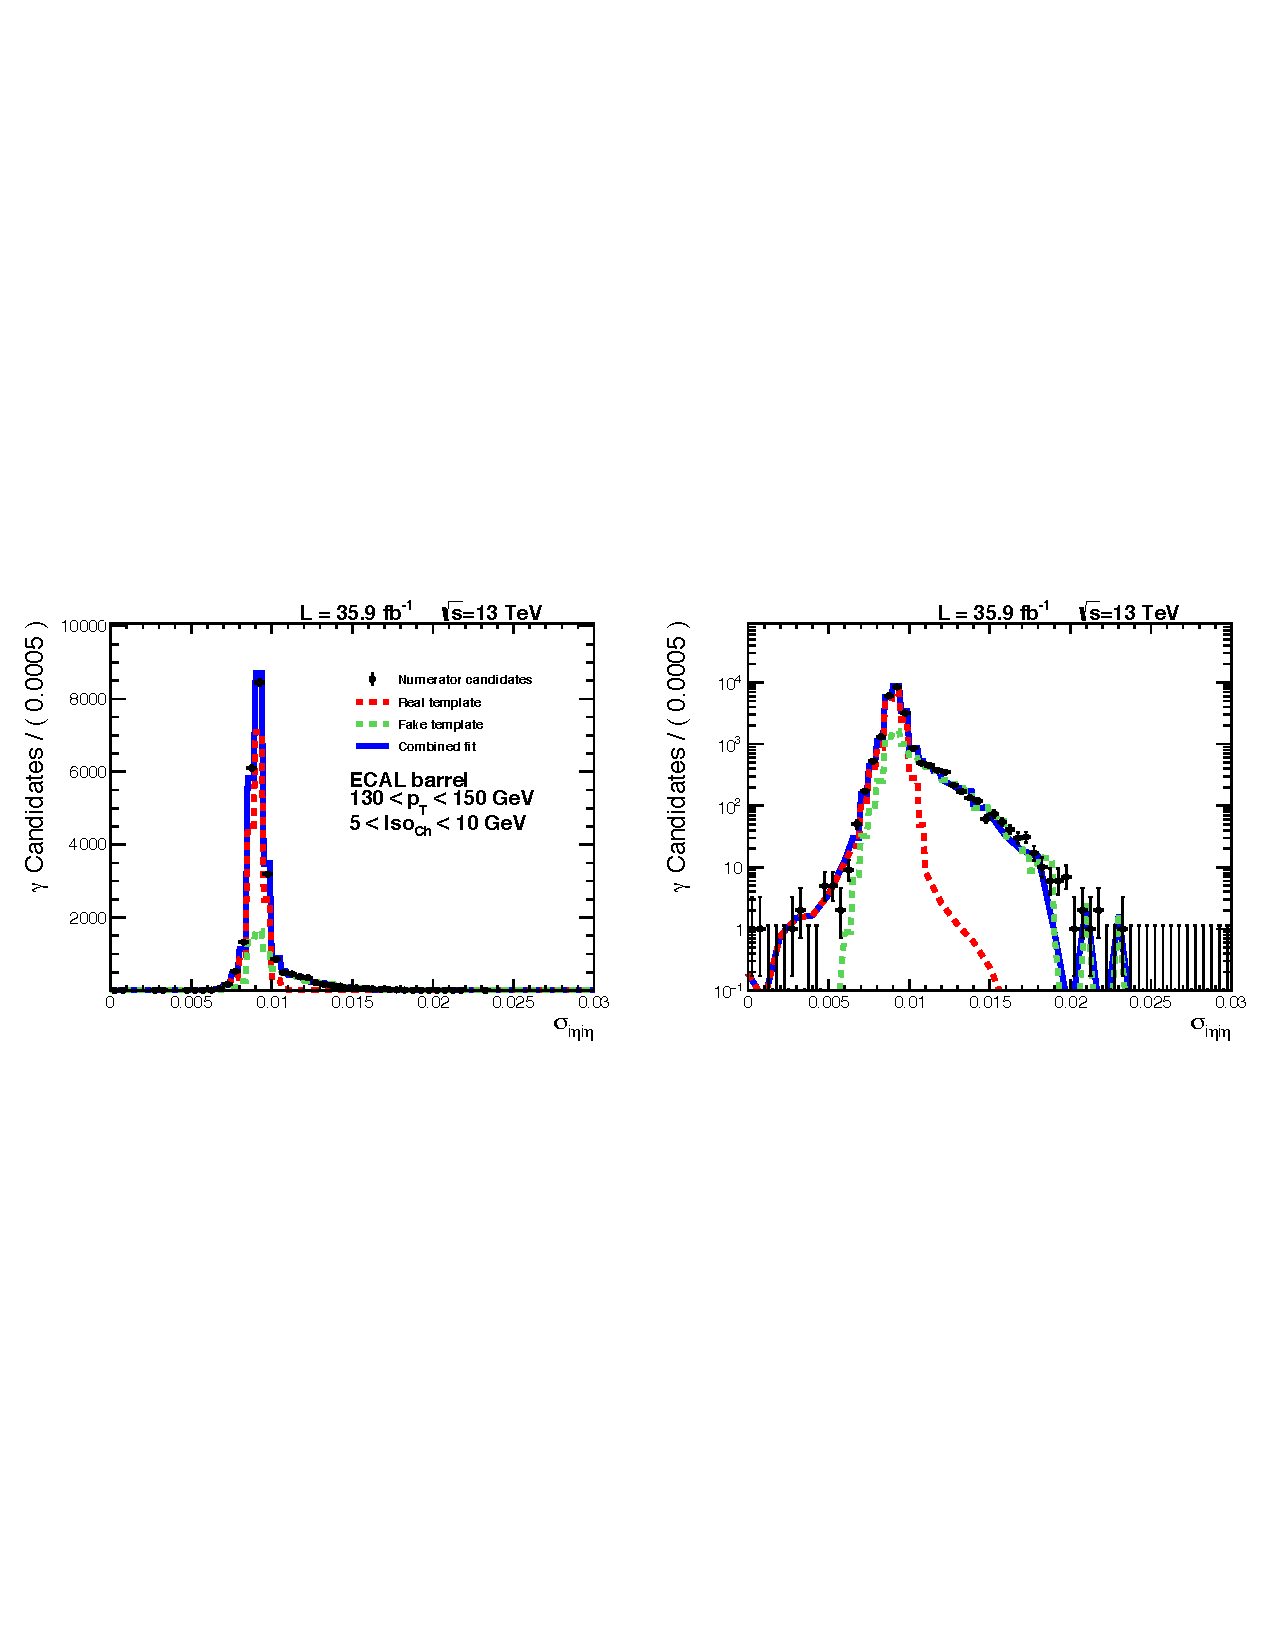
\includegraphics[width=1.0\textwidth]{figures/fakeRatePlotEB_pT130To150_chIso5To10.pdf}
  \caption{A template fit in the EB with $130<\pt<150\GeV$, shown in linear (left) and log (right) scale.}
  \label{fig:template_fit}
\end{figure}

Dividing the numerator yields by the denominator gives the fake rates in the nine \pt bins for both the EB and EE categories, as shown in Fig.~\ref{fig:fake_rate}. These are represented by the black data points with horizontal error bars showing the bin widths. The statistical uncertainties from the denominator distributions and the template fits are represented by the vertical, black error bars. The vertical, blue error bars represent the change in the fake rates under a variation of the \chiso sideband, to be discussed in more detail below in Section~\ref{ss:fr_studies}. The larger fake rate in the EE category is caused by imposing the $\corphoiso < 2.0\GeV$ cut in the denominator selection, which is different for the EB category. The best fit to these fake rate points is shown in red, giving the final fake rate as a function of photon \pt.

\begin{figure}[!htbp]
  \centering
  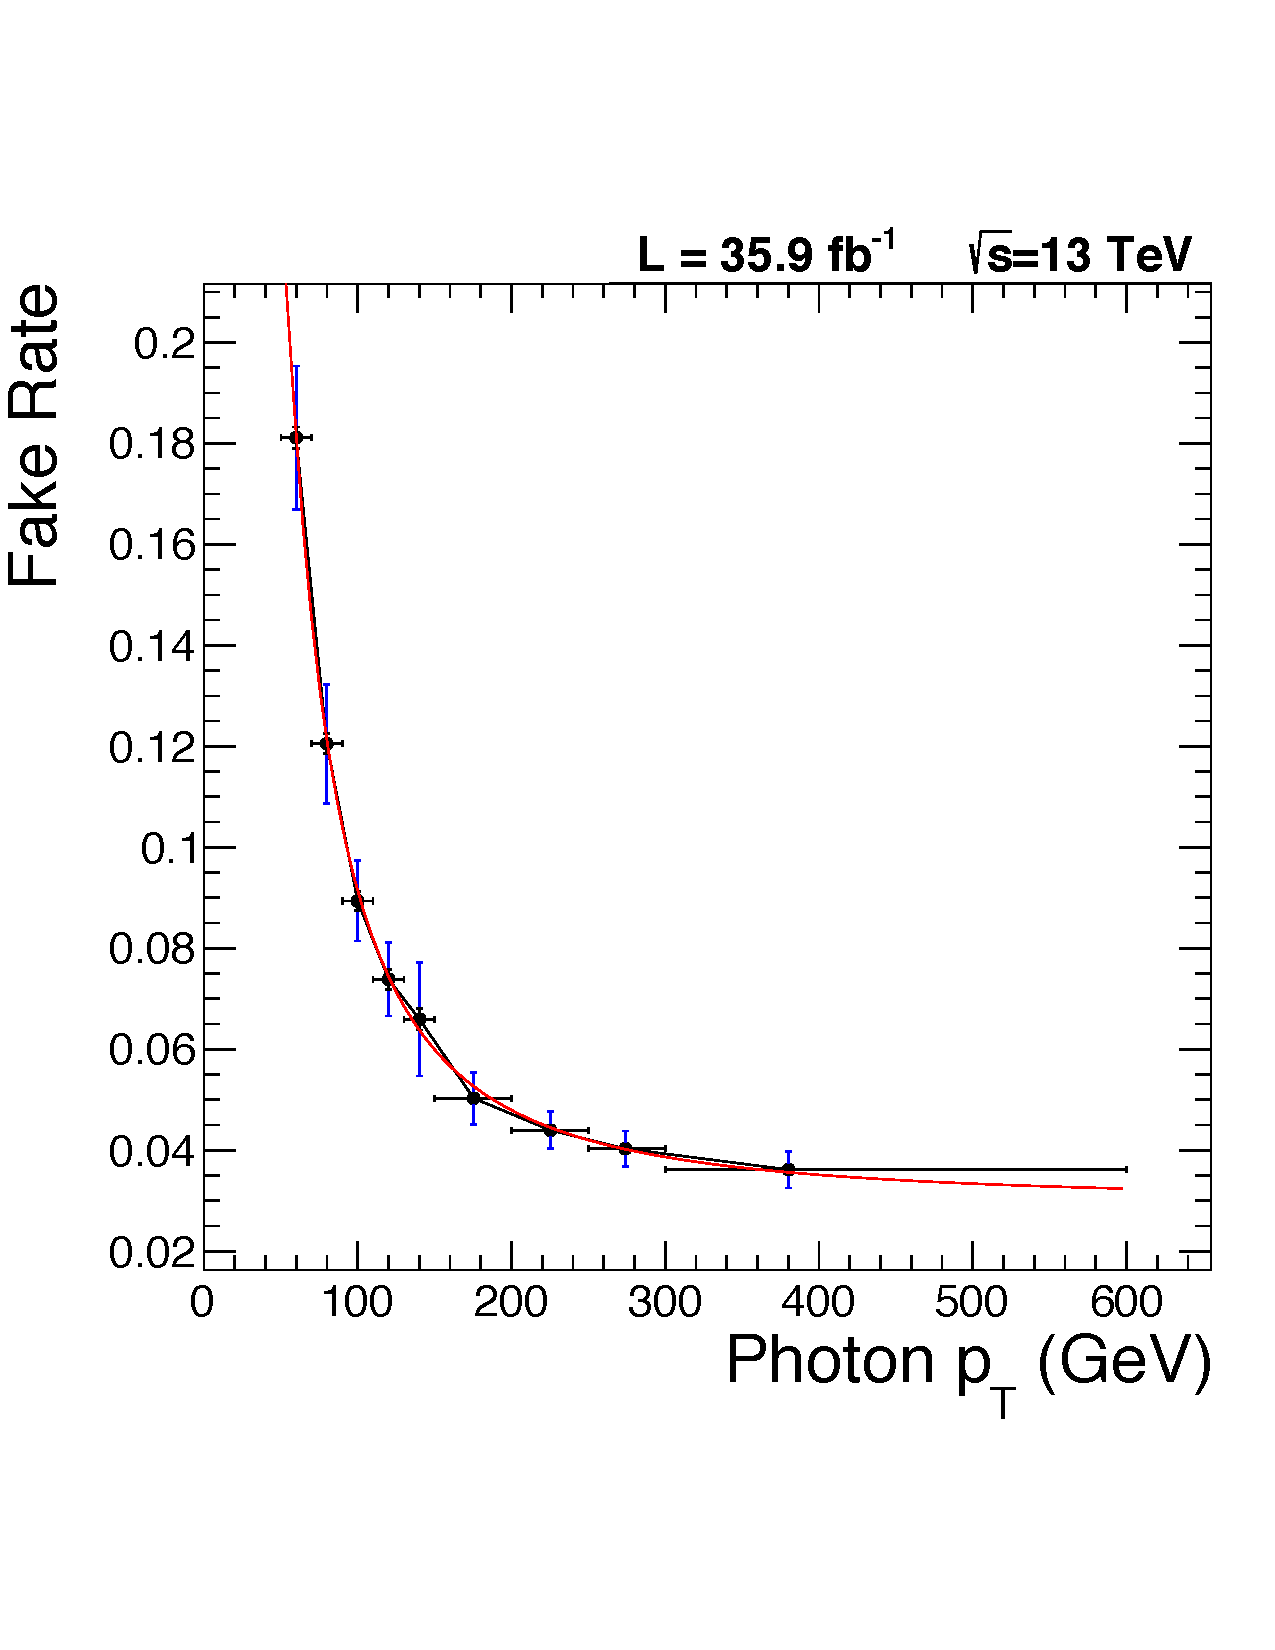
\includegraphics[width=0.49\textwidth]{figures/EBfit2016.pdf}
  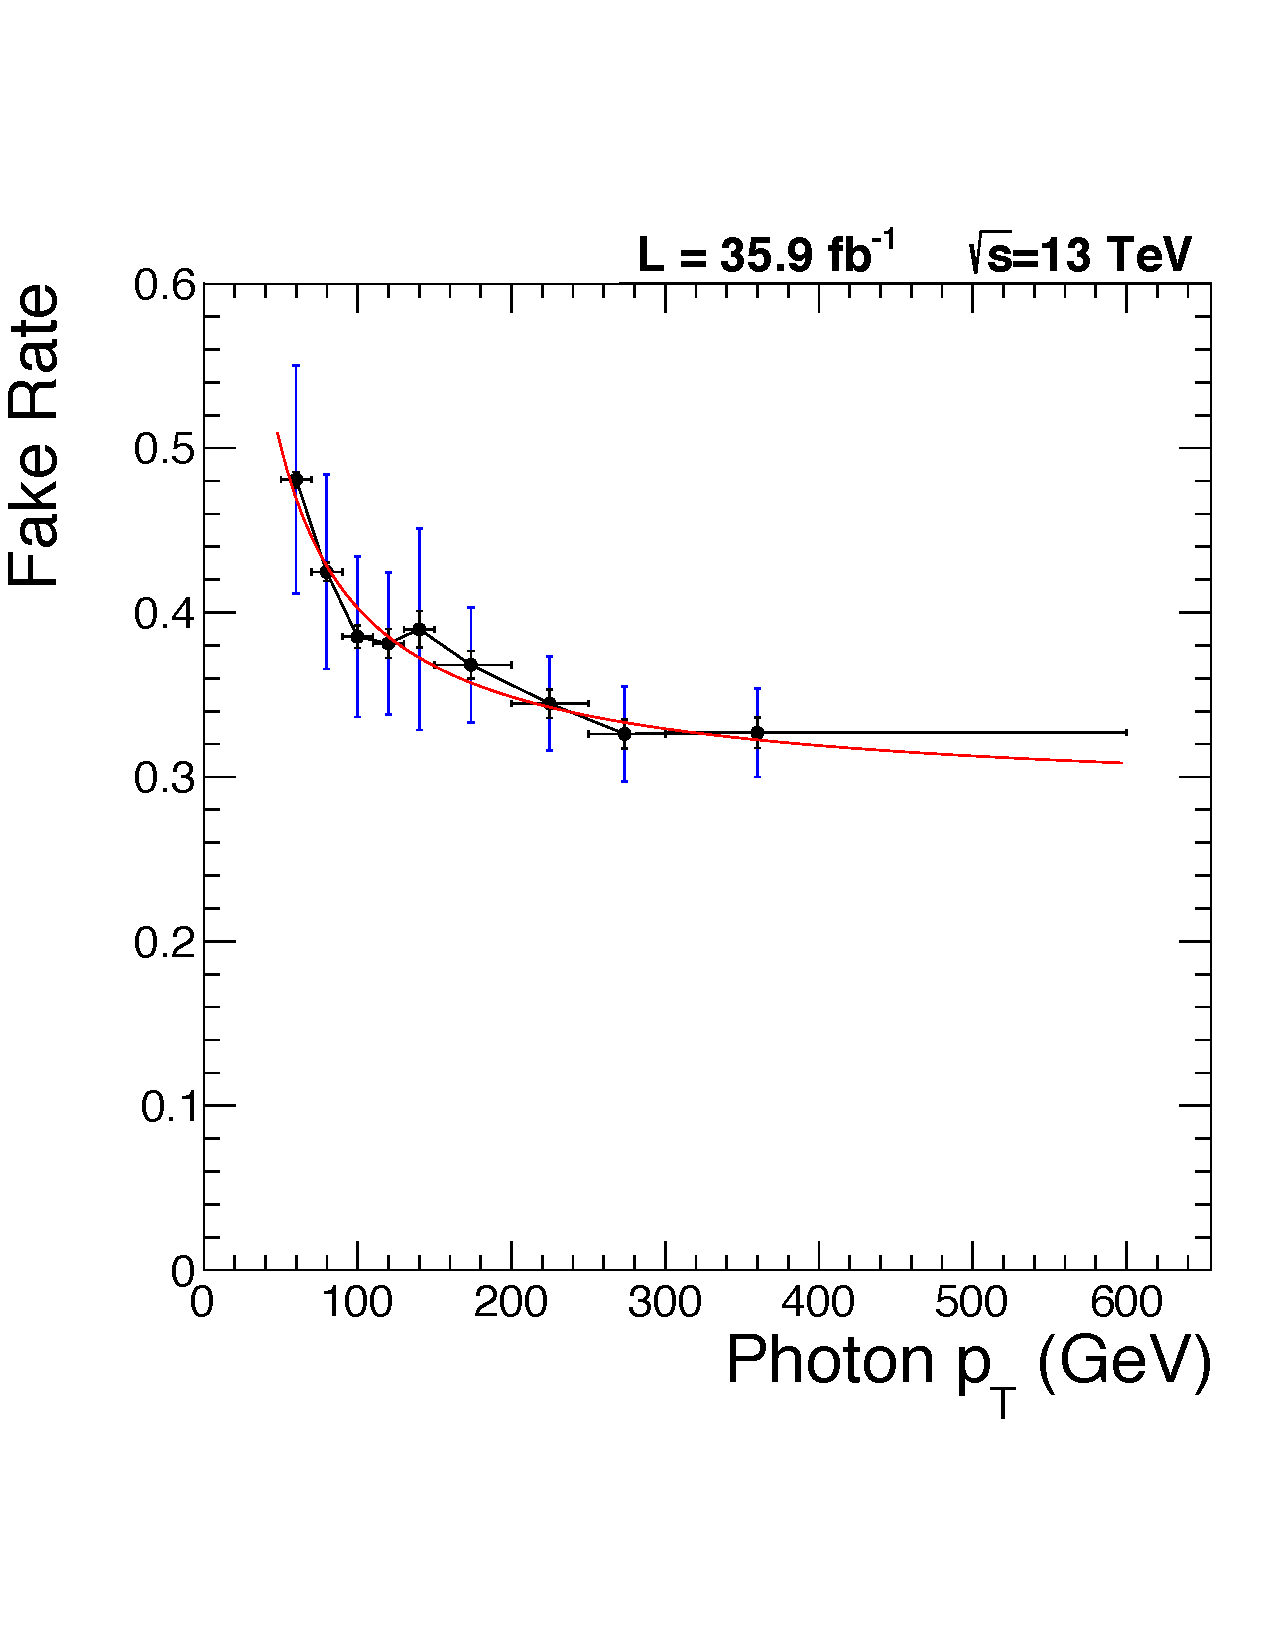
\includegraphics[width=0.49\textwidth]{figures/EEfit2016.pdf}
  \caption{The fake rate in different photon \pt bins for the EB (left) and EE (right) categories. The fake rate function (red) is the best fit to the points.}
  \label{fig:fake_rate}
\end{figure}

The fake rate is parameterized by an inverse function with three free parameters $p_0$, $p_1$, and $p_2$ of the form
\begin{equation}\label{eqn:fake_rate_fn}
  f(\pt) = p_0 + \frac{p_1}{\pt^{p_2}}
\end{equation}
These free parameters are determined by the best fit to the fake rate points taking into account the black statistical error bars shown in Fig.~\ref{fig:fake_rate}. The fit parameters are tabulated in Table~\ref{tab:fit_param}, separately for the EB and EE categories.

\begin{table}[!htbp]
  \caption{Fit parameters for the fake rate function.}
  \label{tab:fit_param}
  \centering
  \vspace{\baselineskip}
  \begin{tabular}{r|cc}
    \hline
    \hline
          & EB        &  EE      \\
    \hline
    $p_0$ & \correction{$0.030\pm0.006$} & \correction{$0.28\pm0.05$} \\
    $p_1$ & \correction{$205.9\pm401.4$}   & \correction{$6.36\pm9.77$}  \\
    $p_2$ & \correction{$1.76\pm0.44$}   & \correction{$0.86\pm0.41$} \\
    \hline
    \hline
  \end{tabular}
\end{table}

The fake rate points shown in Fig.~\ref{fig:fake_rate} are actually the result of deriving separate fake rates from the jet- and muon-triggered datasets and taking their average. To help reduced trigger bias in the jet-triggered dataset, the objects passing the high-\pt photon ID are required to be matched within $\Delta R < 0.6$ to the leading jet within the dataset. The separate fake rates from these two datasets are shown in Fig.~\ref{fig:separate_fake_rates}. Their average is also shown, which is the same as the fake rate in Fig.~\ref{fig:fake_rate}.

\begin{figure}[!htbp]
  \centering
  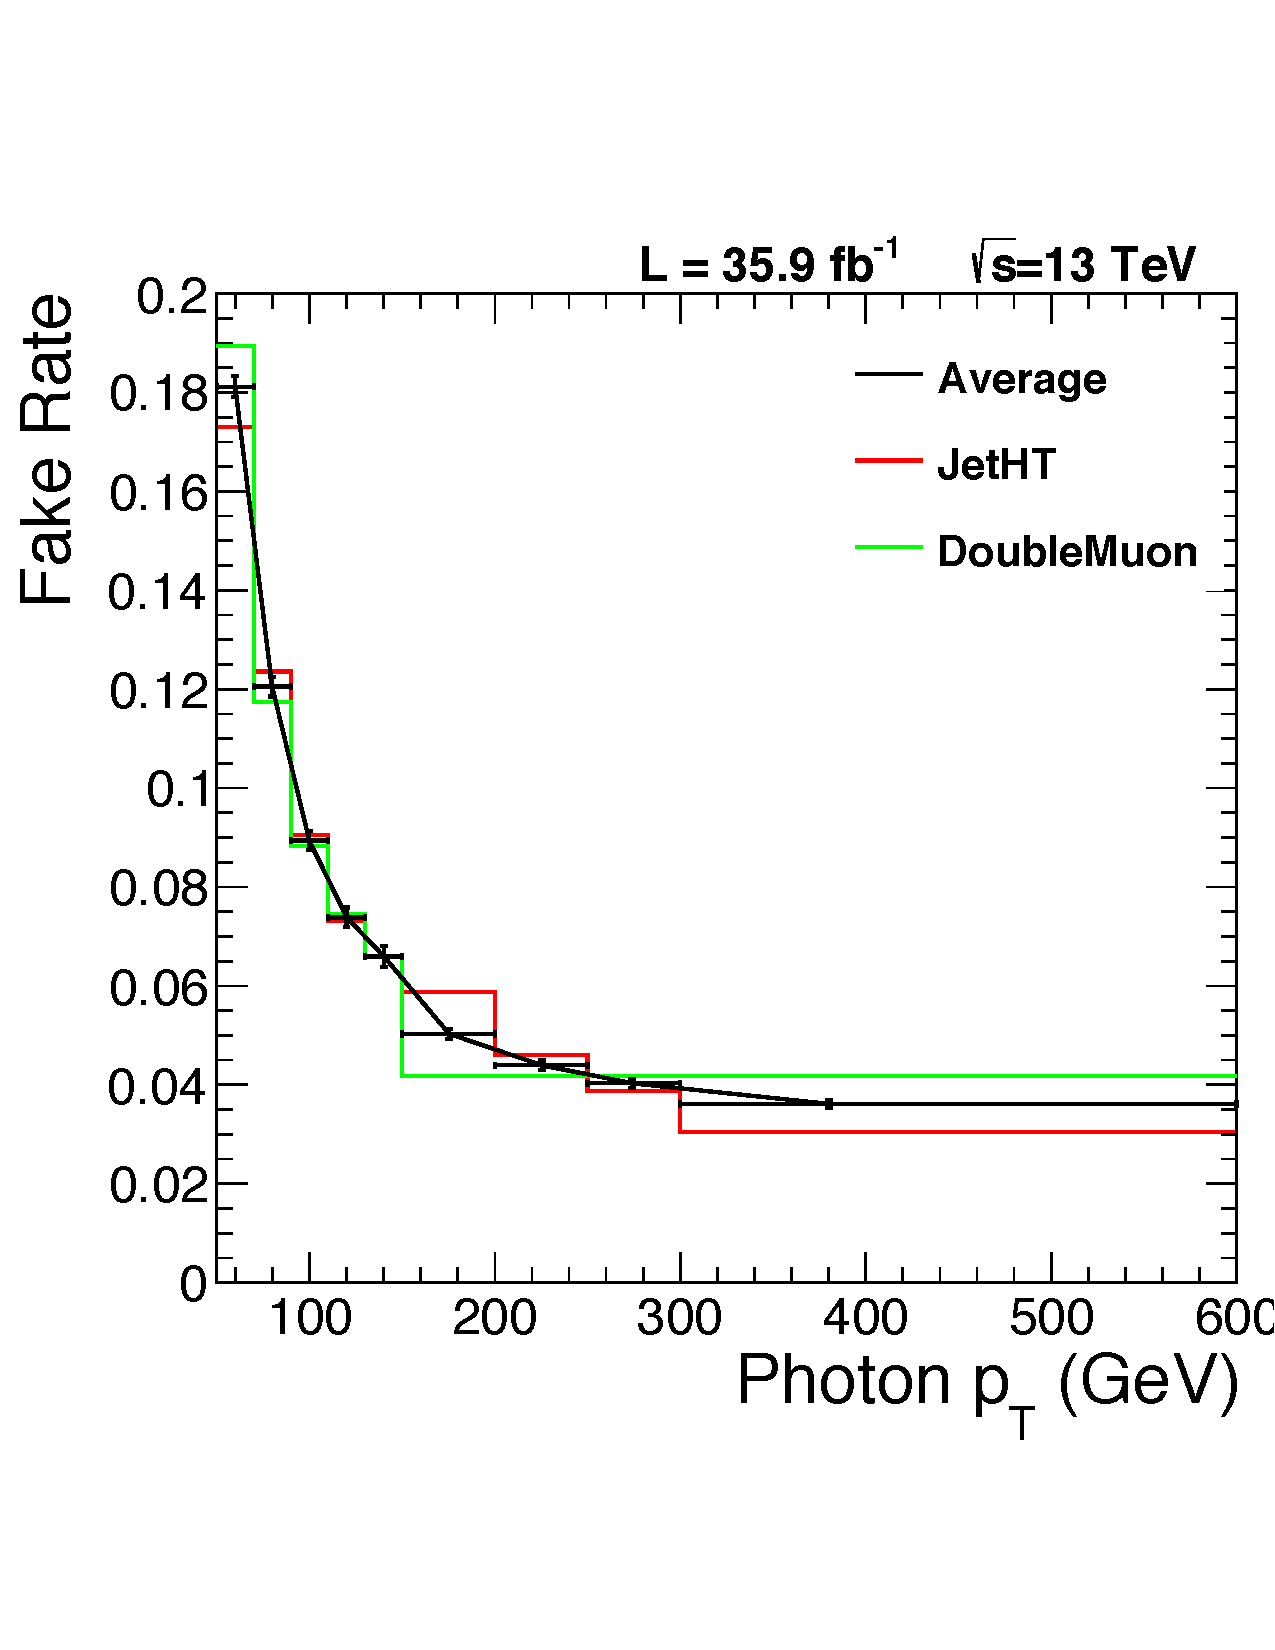
\includegraphics[width=0.49\textwidth]{figures/datasetcompEB_2016.pdf}
  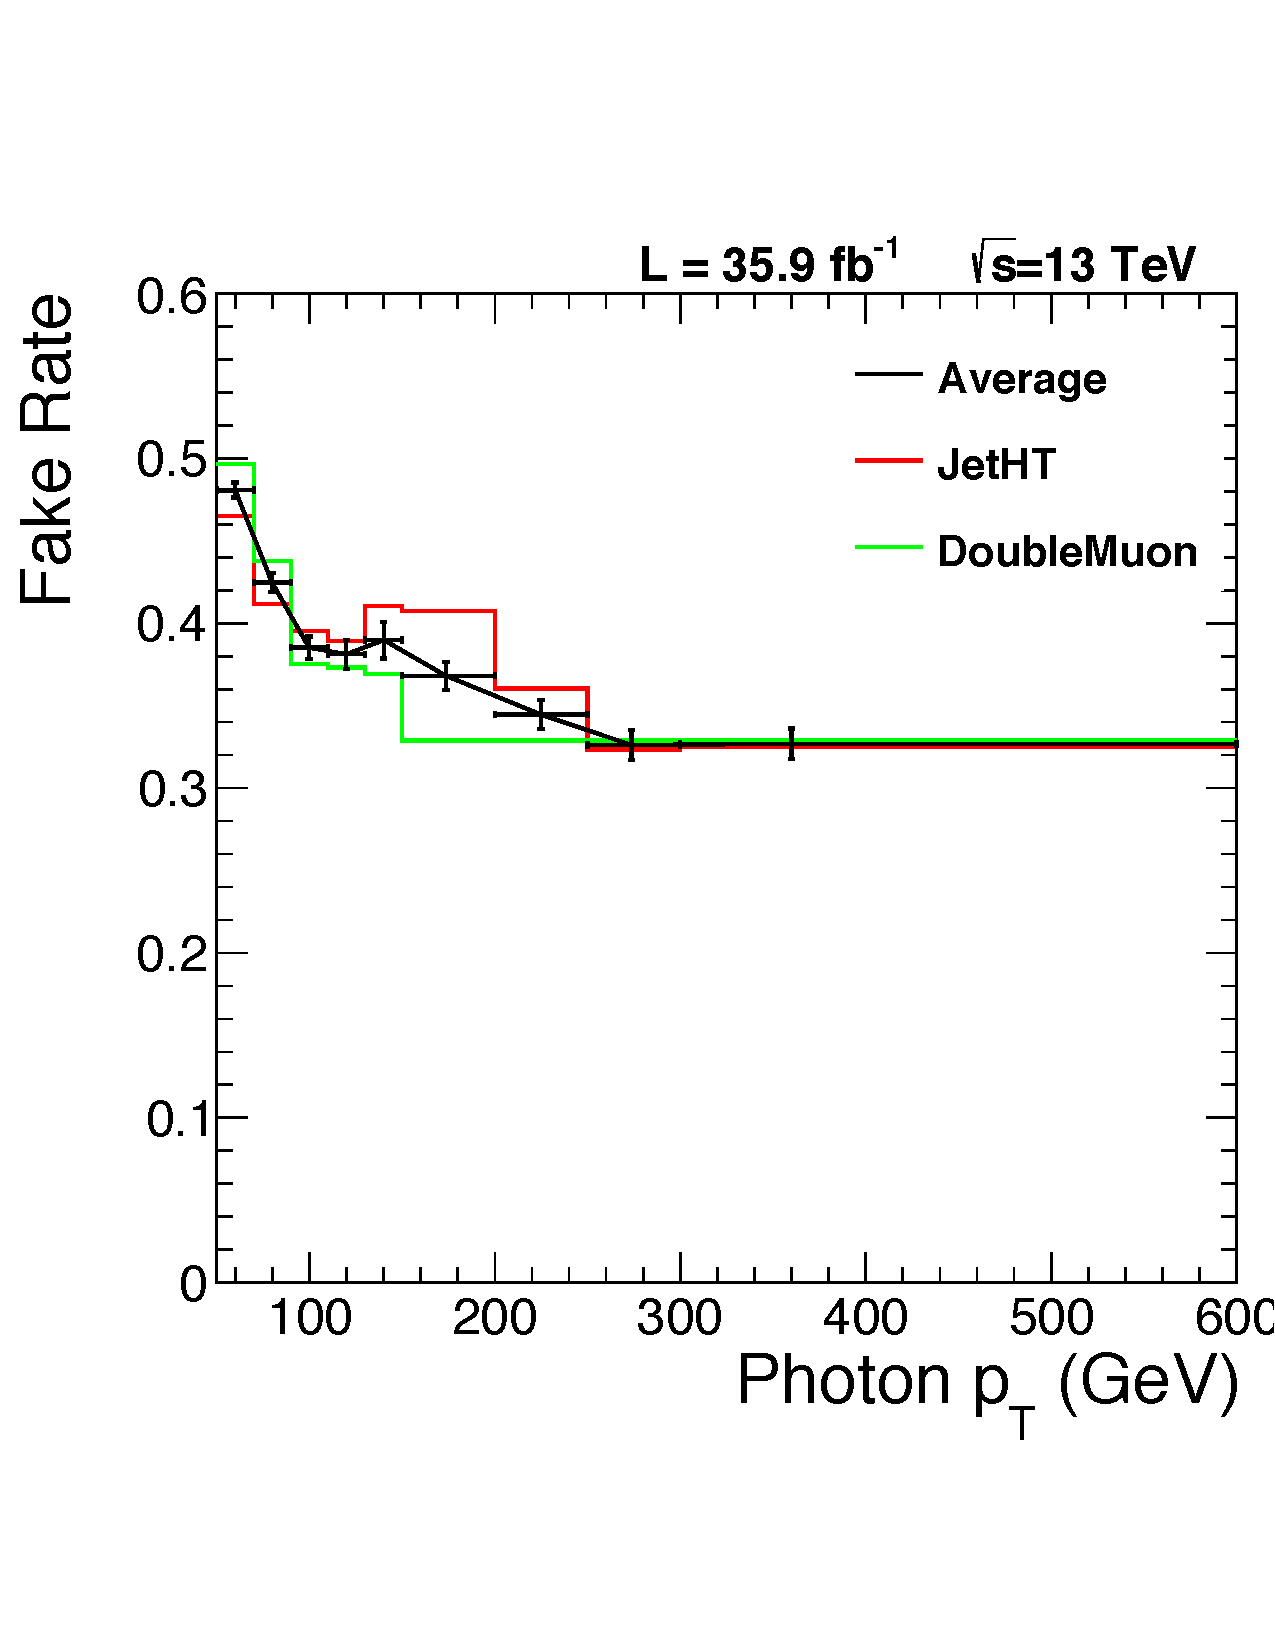
\includegraphics[width=0.49\textwidth]{figures/datasetcompEE_2016.pdf}
  \caption{Separate fake rates for the jet- (red) and muon-triggered (green) datasets are shown in each photon \pt bin for the EB (left) and EE (right) categories. The average of the two (black) is the final fake rate.}
  \label{fig:separate_fake_rates}
\end{figure}


\subsection{Fake Rate Studies}\label{ss:fr_studies}

The effect of jet flavor on the fake rate has been considered in the above calculation. Here we check how robust the fake rate is among other considerations. We check its variation with pileup, change of template variable, and change in sideband definition. These effects are covered with a systematic uncertainty on the overall analysis and will be discussed in Chapter~\ref{ch:systematics}.

The fake rate is sensitive to the amount of pileup in an event. One measure for this is the number of primary vertices (PVs) within an event. In addition to the selection criteria imposed for primary vertex reconstruction, described in Section~\ref{sec:event_reco}, we further require PVs to have
\begin{itemize}
  \item $n_{\text{dof}} \ge 2$;
  \item $|z| < 24$ cm; and
  \item $d_0 \le 2$ cm;
\end{itemize}
\noindent where $n_{\text{dof}}$ is the number of degrees of freedom, $z$ is the $z$-coordinate, and $d_0$ is the impact parameter of the vertex. The $n_{\text{dof}}$ is a criteria used in the vertex fitting algorithm based on weights assigned to the reconstructed tracks, indicating track compatibility with the vertex. Fig.~\ref{fig:nvertices} shows the number of PVs for events in the jet-triggered dataset containing at least one photon passing the high-\pt photon ID. The distribution is shown both before and after these PV quality cuts are imposed.

\begin{figure}[!htbp]
  \centering
  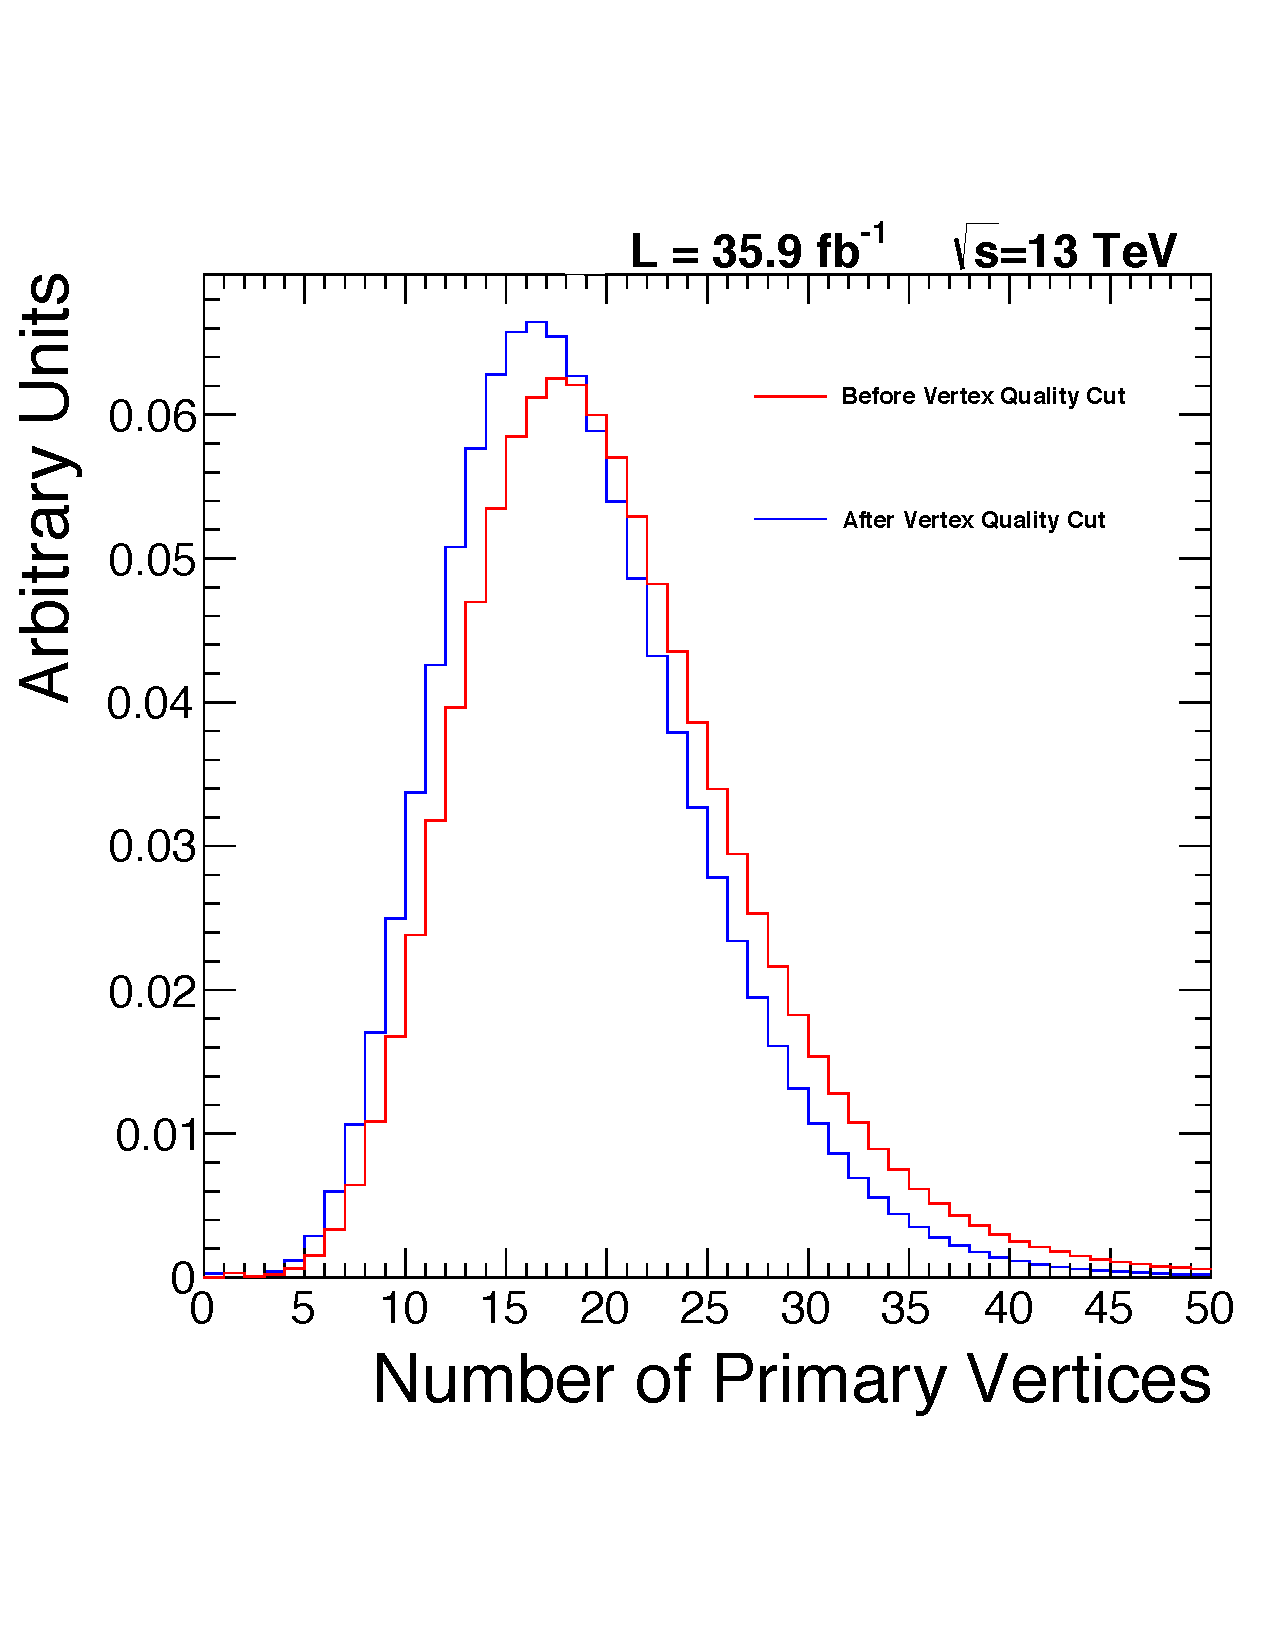
\includegraphics[scale=0.38]{figures/vtxComp2016.pdf}
  \caption{The number of PVs for events containing at least one photon in the jet-triggered dataset used for the fake rate calculation. The distributions are shown before (red) and after (blue) further filtering of the PVs is imposed.}
  \label{fig:nvertices}
\end{figure}

Based on these distributions of PVs, the fake rate calculation was performed using the jet-triggered dataset in bins containing events with 0-13, 14-17, 18-20, 21-24, and 25 or more PVs. These bins were chosen to span the range and offer an approximately uniform amount of statistics within each bin. The results are shown in Fig.~\ref{fig:fr_pileup} for the EB and EE regions. In general, the fake rate increases with the number of PVs.

\begin{figure}[!htbp]
  \centering
  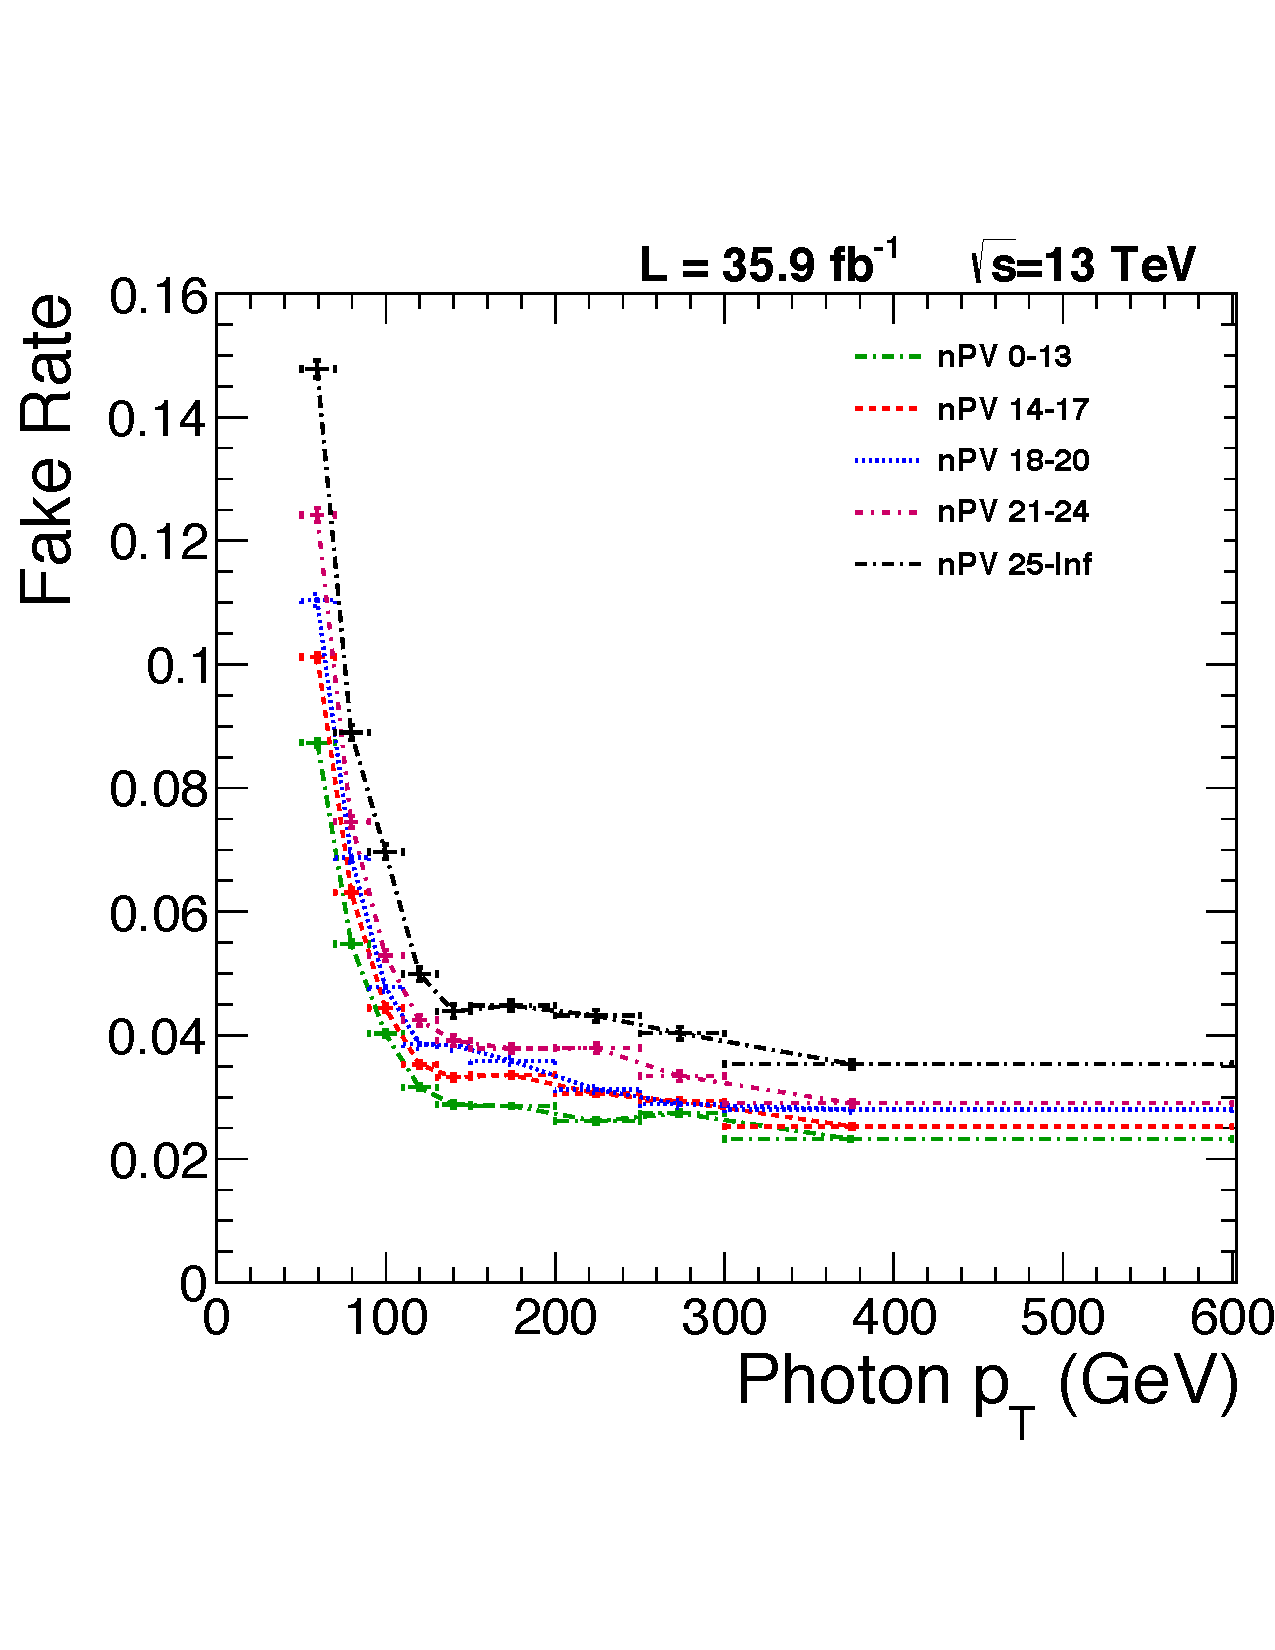
\includegraphics[width=0.49\textwidth]{figures/pileup2016CompEB}
  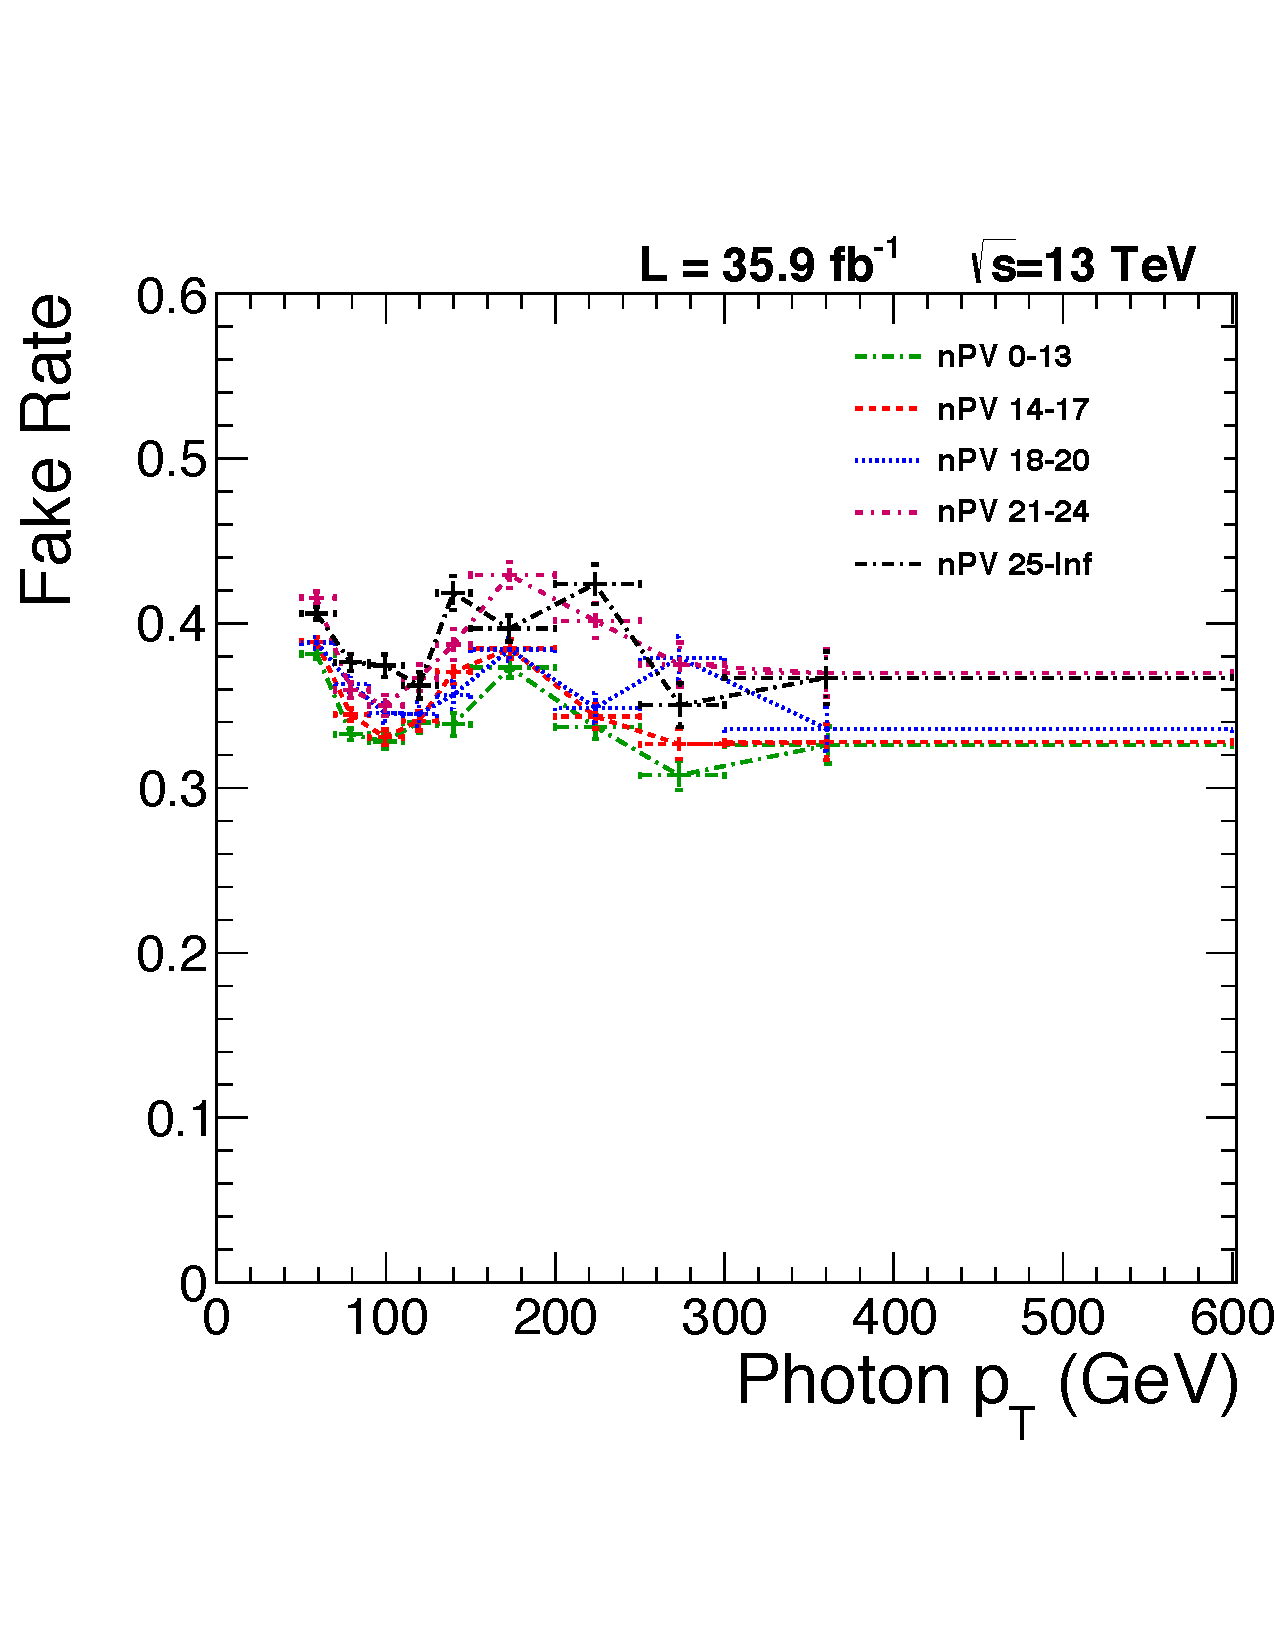
\includegraphics[width=0.49\textwidth]{figures/pileup2016CompEE}
  \caption{The fake rate based on the number of PVs in the events using the jet-triggered dataset in the EB (left) and EE (right).}
  \label{fig:fr_pileup}
\end{figure}

Another assessment of the fake rate results in its change from using an alternate choice of template variable. The isolation variable \chiso, like \sieie, is sensitive to the differences between real and fake photons and is the best alternate choice among the photon ID variables. The sideband variable must simultaneously be changed and \sieie is the natural choice. Note, the \chiso and \sieie variables are correlated for fake photons due to the underlying jet fragmentation process, but are largely uncorrelated for real photons. The effect of this correlation is studied using simulation in Section~\ref{sec:fake_templates_closure_test}. The sideband cuts start at their corresponding cut in the photon ID and are $0.0105 < \sieie < 0.0150$ in the EB and $0.0280 < \sieie < 0.0400$ in the EE. Fig.~\ref{fig:fr_template_comparison} shows a comparison of the fakes rates produced considering \chiso and \sieie as separate template variable with the appropriate sideband variable. The fake rates are found to be in close agreement in both the EB and EE categories. Further investigations of this study, along with the templates produced using the \chiso variable in a simulated sample, are presented in the closure test studies detailed in Section~\ref{ssec:closure_test_studies}.

\begin{figure}[!htbp]
  \centering
  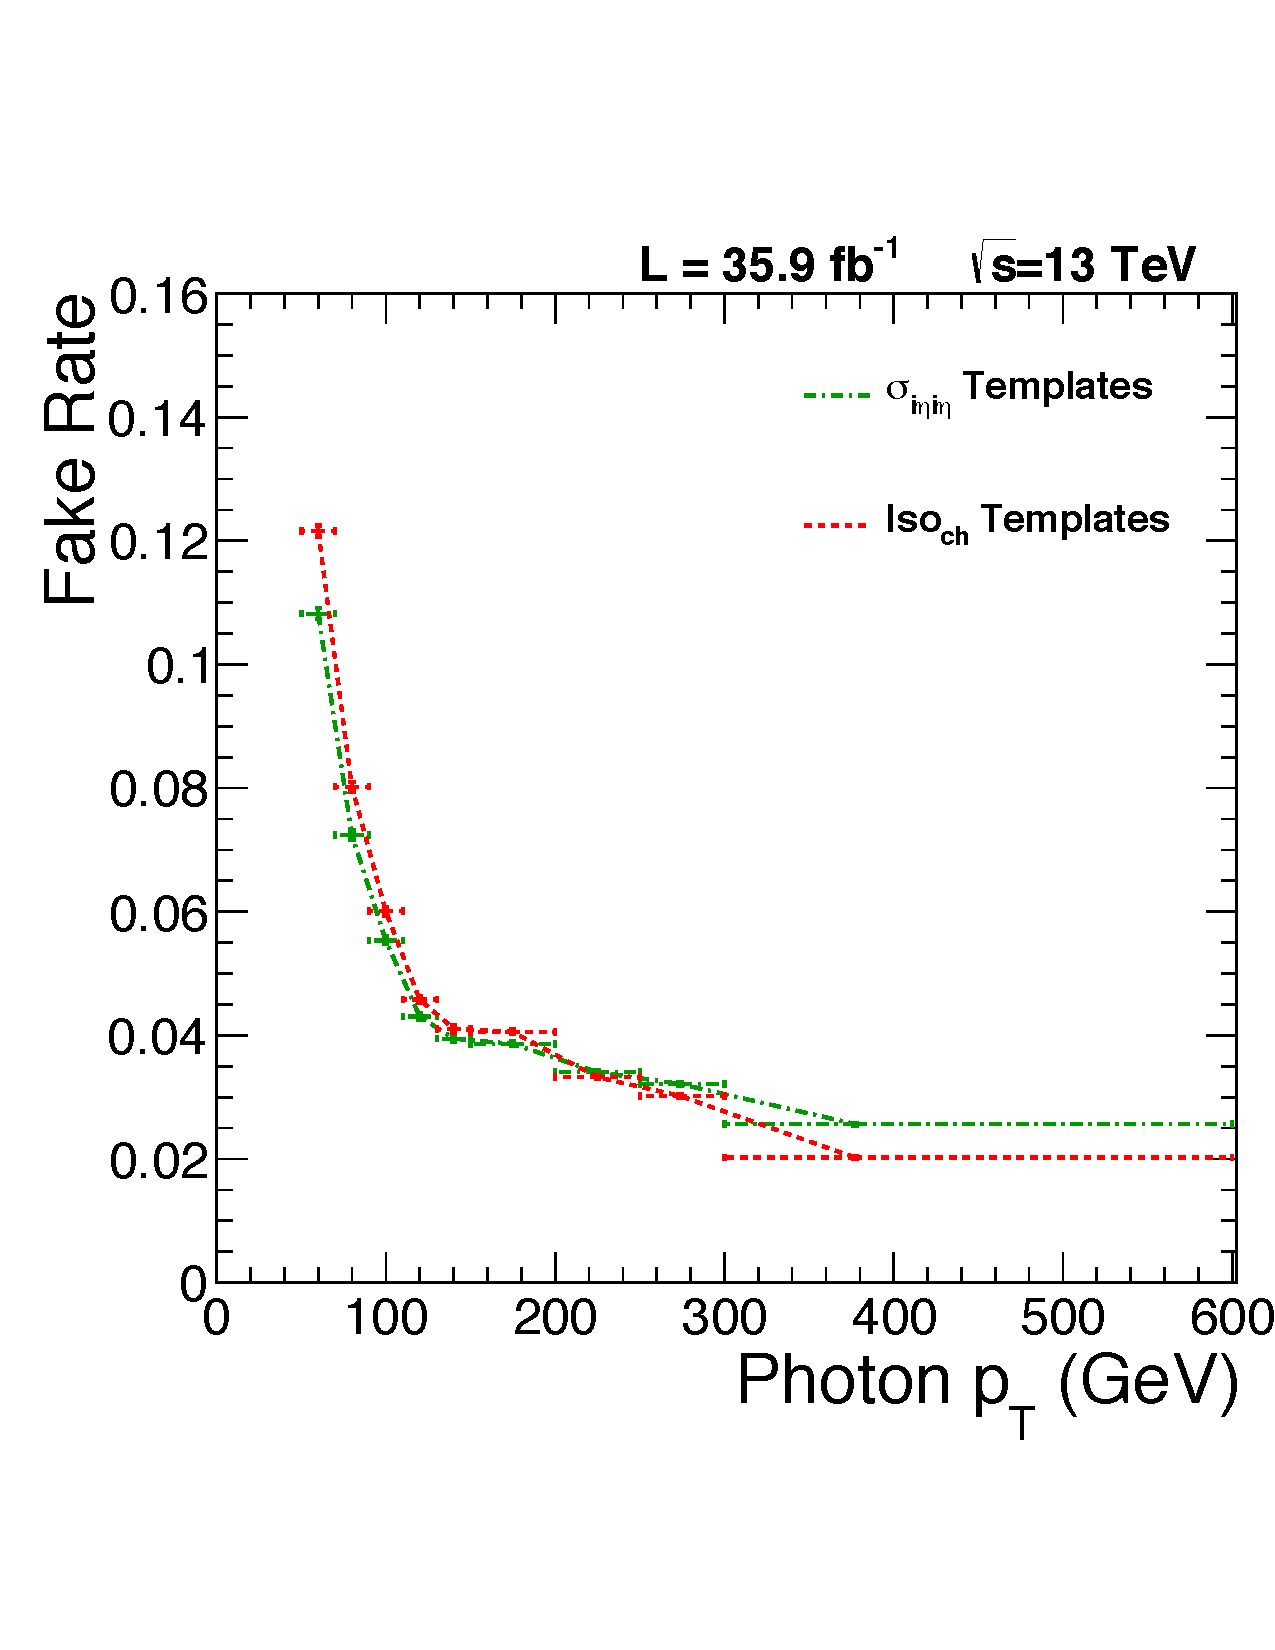
\includegraphics[width=0.49\textwidth]{figures/sieieChIsoCompEB.pdf}
  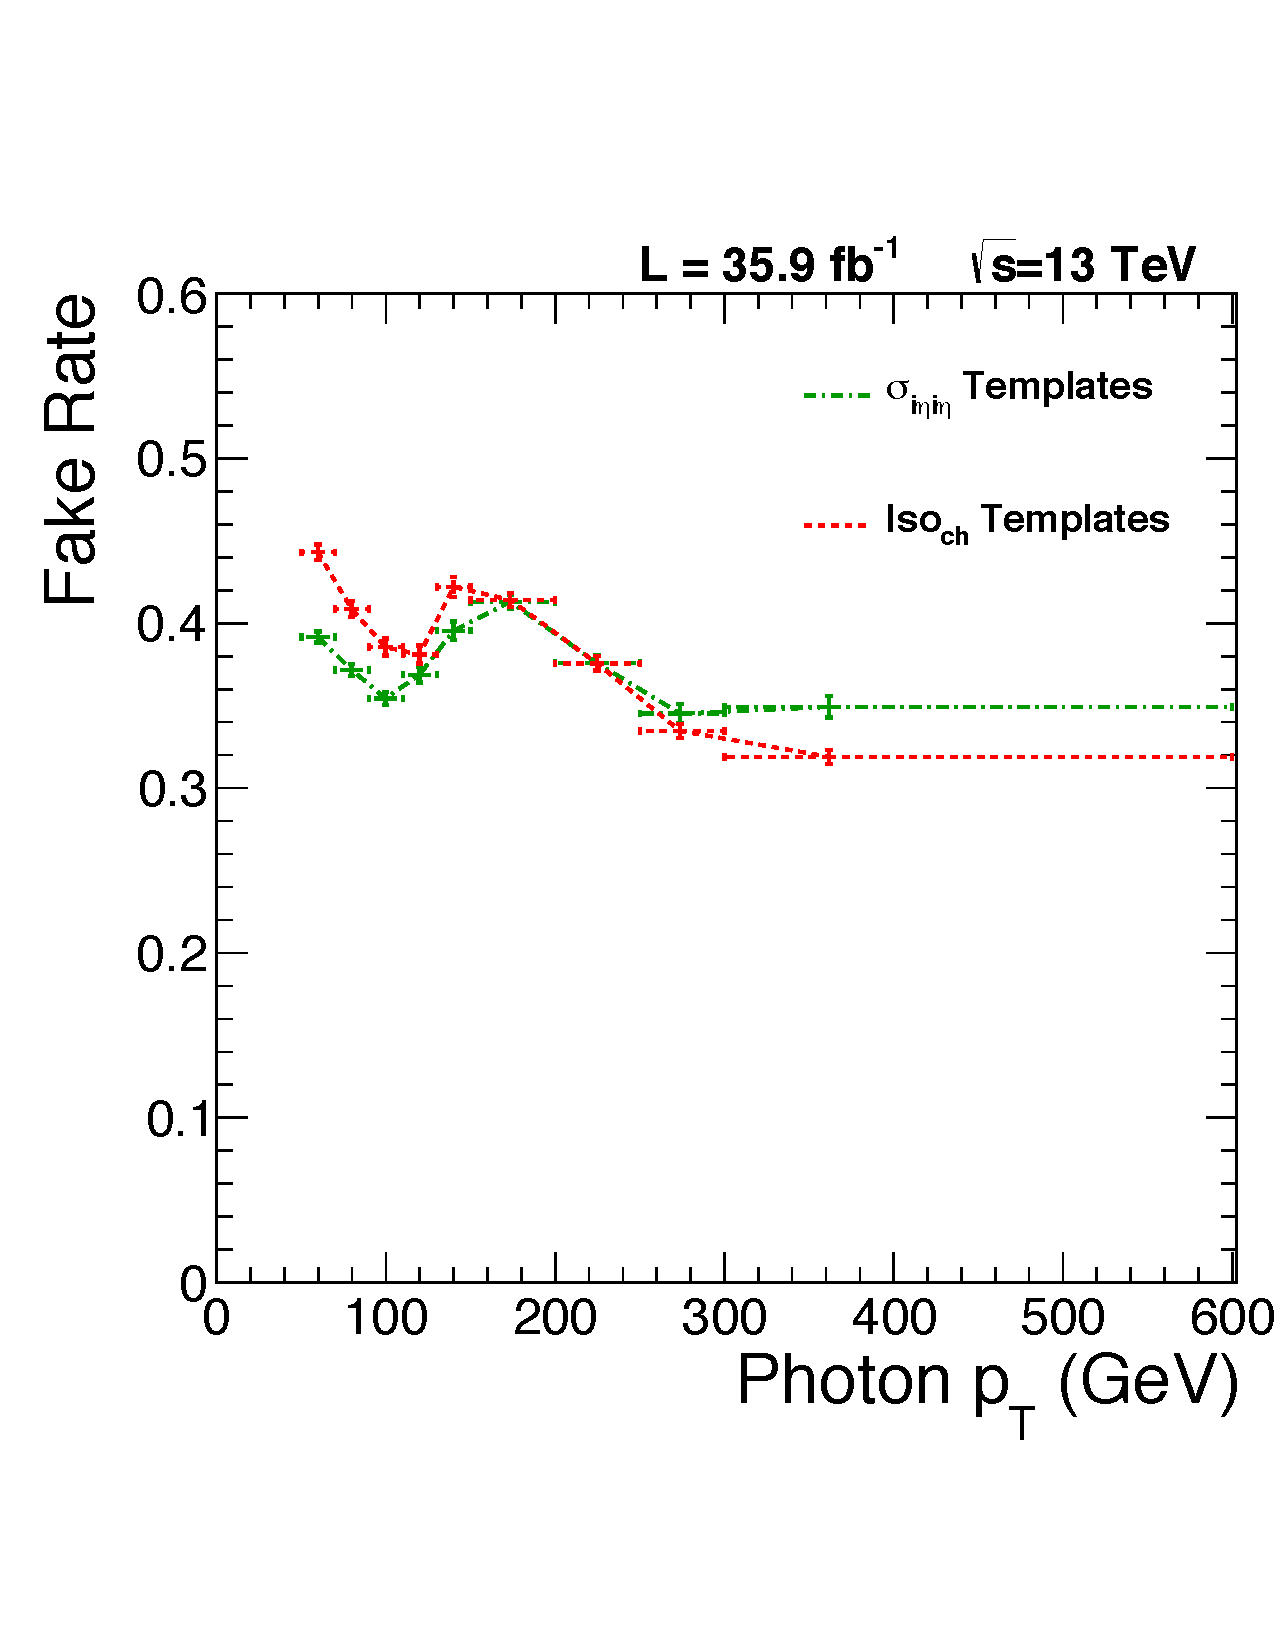
\includegraphics[width=0.49\textwidth]{figures/sieieChIsoCompEE.pdf}
  \caption{Comparison of the fake rates using \sieie (green) and \chiso (red) template variables in the EB (left) and EE (right).}
  \label{fig:fr_template_comparison}
\end{figure}

The choice of cuts for the sideband also affects the fake rate. When using \chiso as the template variable, three different \sieie sideband choices are considered in each ECAL region: 0.0105-0.0150, 0.0105-0.2000 and 0.0105-1.0000 in the EB and 0.0280-0.0400, 0.0400-0.0600, and 0.028-1.000 in the EE. Fig.~\ref{fig:fr_chiso_sideband_variation} shows the variation of the fake rate using these sideband choices in each category. Differences are observed between the orthogonal sideband choices. Further investigation of this effect will be considered during the closure test study below, including the variation using the \chiso sidebands.

\begin{figure}[!htbp]
  \centering
  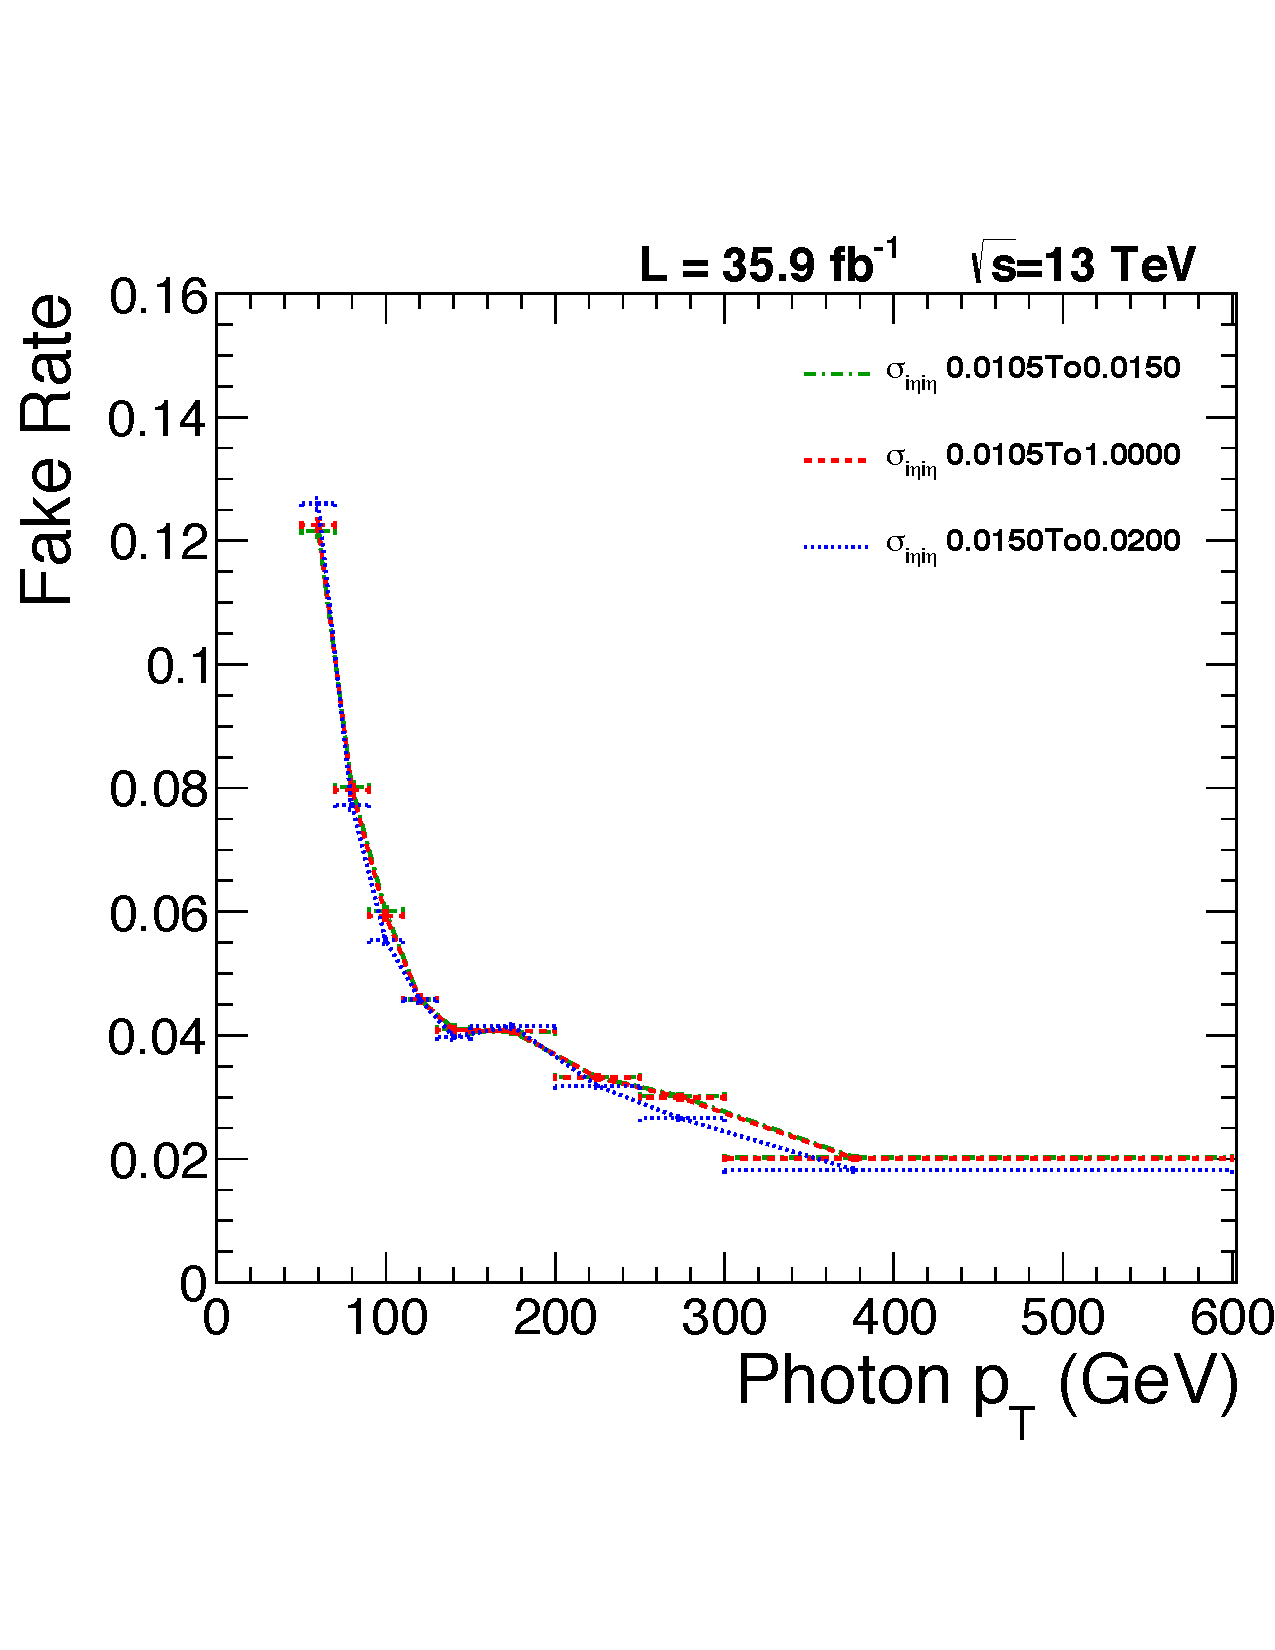
\includegraphics[width=0.49\textwidth]{figures/chIsoFRCompEB.pdf}
  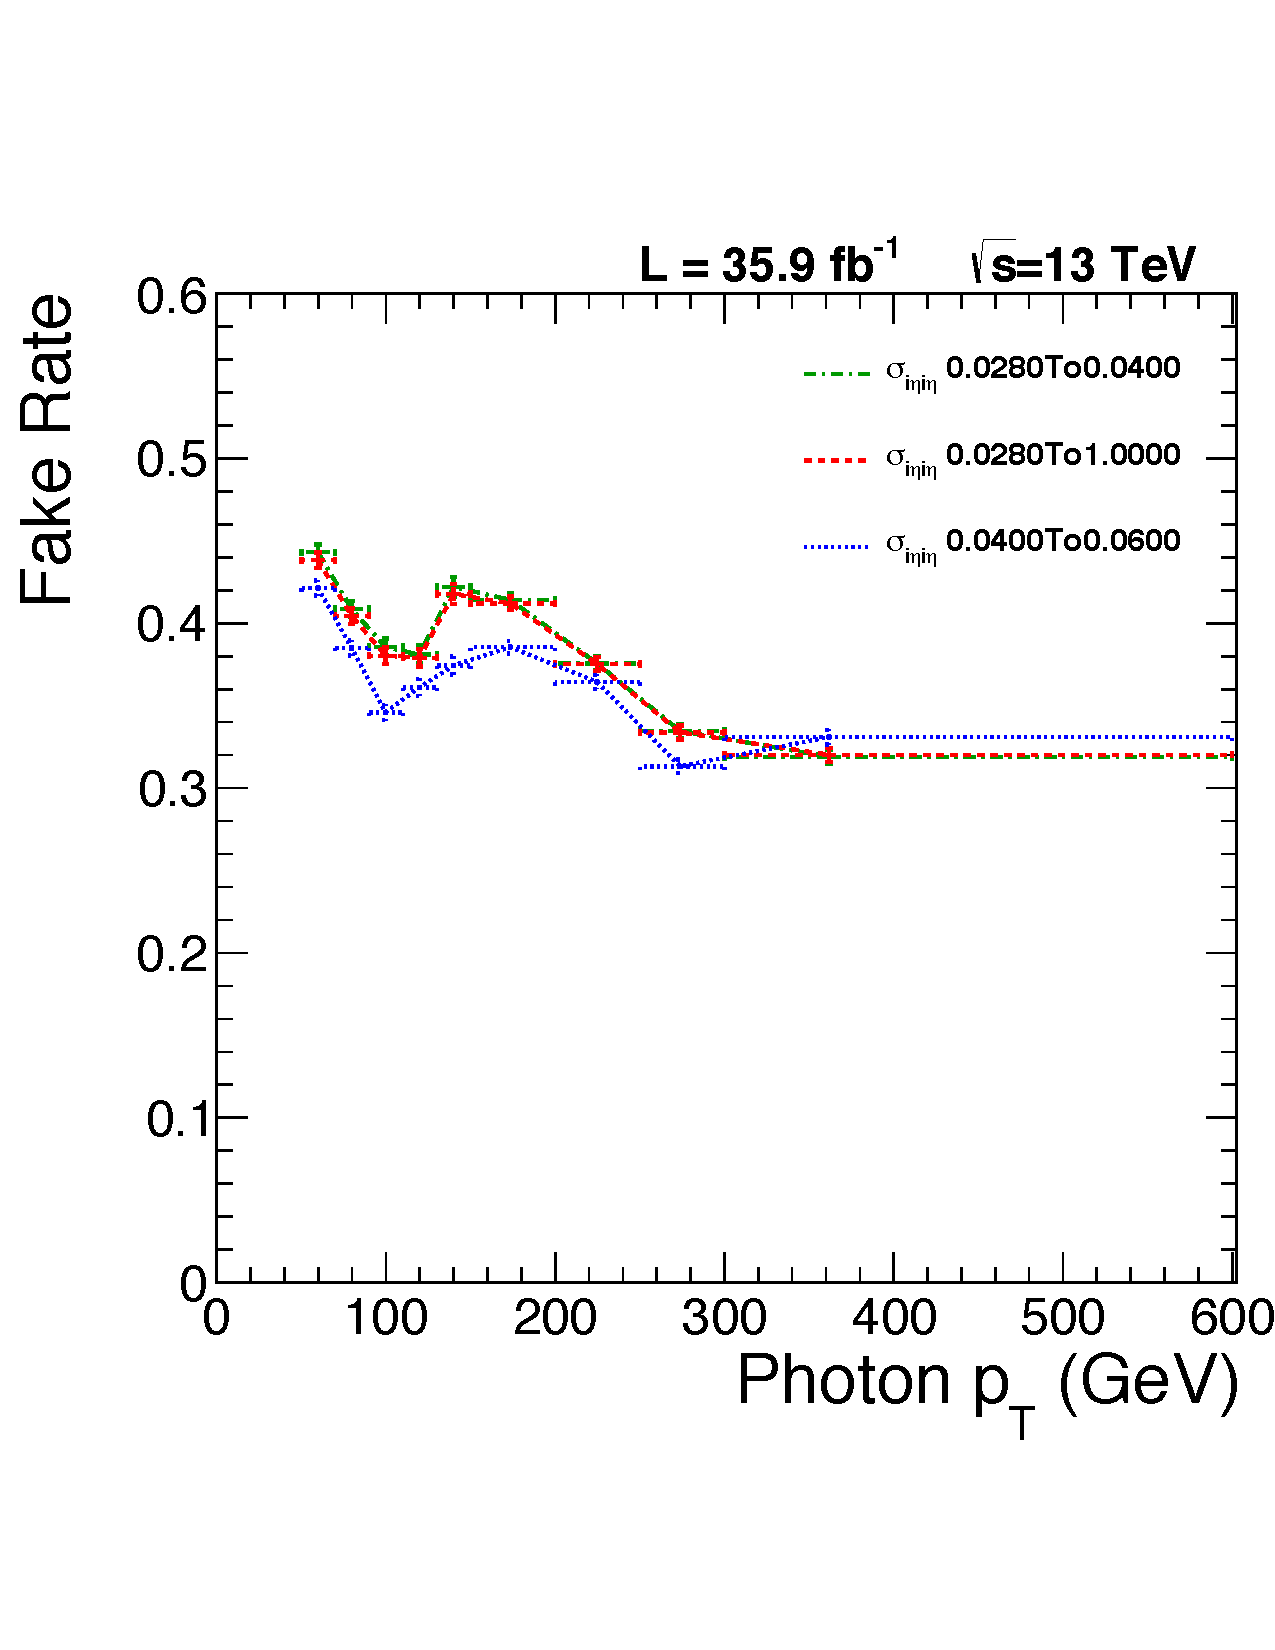
\includegraphics[width=0.49\textwidth]{figures/chIsoFRCompEE.pdf}
  \caption{The fake rate using a \chiso template with variations in the \sieie sideband for the EB (left) and EE (right).}
  \label{fig:fr_chiso_sideband_variation}
\end{figure}


\subsection{Applying the Fake Rate Method}

The fake rate function $f$ in Eq.~(\ref{eqn:fake_rate_fn}) can now be applied to events in the diphoton data sample. Events are selected with two objects passing either the high-\pt photon ID, the denominator definition, or a combination of both. \correction{Let $T$ denote an object passing the photon ID to signify a true photon passing this tight ID, and let $F$ denote an object passing the denominator definition to signify a potential fake photon failing the photon ID / passing this looser ID.} If we label the leading and subleading objects using the index $i=1$ or 2, respectively, then we have 4 categories of events: $T_1T_2$, $T_1F_2$, $F_1T_2$, and $F_1F_2$. Events containing an $F$ object get reweighted by $f$ to be used in the background estimation.

The jj background is estimated by reweighting each of the two $F$ objects for all events in the data sample:
\begin{equation}
  \text{jj} = (f_1F_1)(f_2F_2)
\end{equation}
 \noindent where $f_i$ is the fake rate function $f$ evaluated at the \pt of photon $i$, for $i=1$, 2. The $\gamma$j background estimation takes more care because the $T$ objects are comprised of real photons ($R$) and not real photons ($N$), i.e., $T = R+N$, where $N=fF$. The $\gamma$j background is estimated over all data events according to:
\begin{align}
  \gamma\text{j} &= (R_1N_2)+(N_1R_2) \\
  &= (T_1-f_1F_1)(f_2F_2) + (f_1F_1)(T_2-f_2F_2) \\
  &= T_1(f_2F_2)+(f_1F_1)T_2-2(f_1F_1)(f_2F_2)
\end{align}
\noindent Therefore, the $\gamma$j background is estimated by reweighting the $TF$ and $FT$ samples minus twice the $FF$ sample.


\subsection{Closure Test to the Fake Rate Method}\label{ssec:closure_test}

An MC based approach is used to validate the fake rate method performed for determining the jet-faking-photon rate. The general idea is that we perform the fake rate method on a simulated sample using the same procedure as was used on the data sample. This yields a fake prediction in the simulated sample. Since the simulated sample was produced using an MC calculation, we have access to the MC truth information for the generated particles, which provides information about the event history and properties of these particles. From this information, we can identify which types of particles pass the high-\pt photon ID. In particular, we can determine which particles faked a photon signature in the simulated sample and compare this yield to the fake prediction. The QCD jj and $\gamma$j MC samples listed in Table~\ref{tab:closure_test_samples} are produced for collaboration-wide use by the CMS Collaboration and contain a sufficient number of fake photons to be used as the simulated sample for this closure test. The $\gamma$j samples used here are same samples that were used in the real template construction, listed in Table~\ref{tab:real_template_samples}.

\begin{table}[!htb]
  \caption{The Monte Carlo samples and corresponding cross sections used for the closure test to the fake rate method. The full, internal CMS path name is specified by appending the dataset path with \texttt{/RunIISummer16MiniAODv2-\allowbreak PUMoriond17\_\allowbreak 80X\_\allowbreak mcRun2\_\allowbreak asymptotic\_\allowbreak 2016\_\allowbreak TrancheIV\_\allowbreak v6/\allowbreak MINIAODSIM}.}
  \label{tab:closure_test_samples}
  \centering
  \vspace{\baselineskip}
  \small %\footnotesize
  \begin{tabular}{lc}
  \hline \hline
  Dataset path & Cross section (pb) \\ 
  \hline
  /QCD\_Pt\_50to80\_TuneCUETP8M1\_13TeV\_pythia8 & 19204300 \\
  /QCD\_Pt\_80to120\_TuneCUETP8M1\_13TeV\_pythia8 & 2762530 \\
  /QCD\_Pt\_120to170\_TuneCUETP8M1\_13TeV\_pythia8 & 471100 \\
  /QCD\_Pt\_170to300\_TuneCUETP8M1\_13TeV\_pythia8 & 117276 \\
  /QCD\_Pt\_300to470\_TuneCUETP8M1\_13TeV\_pythia8 & 7823 \\
  /QCD\_Pt\_470to600\_TuneCUETP8M1\_13TeV\_pythia8 & 648.2 \\
  /QCD\_Pt\_600to800\_TuneCUETP8M1\_13TeV\_pythia8 & 186.9 \\
  /QCD\_Pt\_800to1000\_TuneCUETP8M1\_13TeV\_pythia8 & 32.293 \\
  /QCD\_Pt\_1000to1400\_TuneCUETP8M1\_13TeV\_pythia8 & 9.4183 \\
  /QCD\_Pt\_1400to1800\_TuneCUETP8M1\_13TeV\_pythia8 & 0.84265 \\
  /QCD\_Pt\_1800to2400\_TuneCUETP8M1\_13TeV\_pythia8 & 0.114943 \\
  /QCD\_Pt\_2400to3200\_TuneCUETP8M1\_13TeV\_pythia8 & 0.00682981 \\
  /QCD\_Pt\_3200toInf\_TuneCUETP8M1\_13TeV\_pythia8 & 0.000165445 \\
  \hline
  /GJets\_HT-40To100\_TuneCUETP8M1\_13TeV-madgraphMLM-pythia8 & 2.121e+04 \\
  /GJets\_HT-100To200\_TuneCUETP8M1\_13TeV-madgraphMLM-pythia8 & 9.863e+03 \\
  /GJets\_HT-200To400\_TuneCUETP8M1\_13TeV-madgraphMLM-pythia8 & 2.298e+03 \\
  /GJets\_HT-400To600\_TuneCUETP8M1\_13TeV-madgraphMLM-pythia8 & 2.816e+02 \\ 
  /GJets\_HT-600ToInf\_TuneCUETP8M1\_13TeV-madgraphMLM-pythia8 & 9.465e+01 \\
  \hline \hline
  \end{tabular}
\end{table}

The \SHERPA $\gamma\gamma$ background prediction described in Section~\ref{sec:real_background} takes into account the direct photon contribution due to the fragmentation of quarks and gluons according to Ref.~\cite{Hoeche:2009xc}. This suggests that the fakes we need to account for are those coming directly from hadron decays, such as from $\pi^0$ or $\eta$ meson decays. The procedure for identifying these fake photons in the simulated sample is by using the MC truth information associated with the generated particles, as described in the following way.

Reconstructed photons passing the high-\pt photon ID in the simulated sample are matched to the best final state generated particle within $\Delta R \le 0.1$ around the reconstructed photon. There may not be any match within this cone. If the reconstructed photon is matched directly to a final state generator-level hadron, then it is considered fake. If instead the reconstructed photon is matched to a final state generator-level photon, then the generated photon's mothers are used to determine whether or not it is fake. Since in general a generated particle can have multiple mothers within the \SHERPA framework, its sole mother is chosen from the best match in $\Delta R$ among all of its mothers. If the generated photon's mother is matched to a generated hadron, then the reconstructed photon is considered fake. This approach isolates the fake photons from hadron decays and, for example, ignores prompt photons directly from the hard interaction.

The validation of the fake rate method is done in three steps. In each case, the method is performed on the simulated sample, treating it as if it were data, which gives a prediction that can be compared to the correct result obtained using the MC truth information on the same sample. First, the accuracy of fake templates produced using the sideband method is tested by comparing the fake templates obtained in simulation using the sideband definition, as done in data, with the fake template that is obtained using the MC truth information. Second, we test the use of the templates to fit the discriminator variable and extract the fake yields. This is done by performing the fitting procedure on the simulation in the same manner as done in data and comparing against the actual fake yields using the MC truth information, both as a function of \pt. Third, we test the validity of using reweighted denominator objects to predict the kinematics of actual known fakes---in particular, the diphoton invariant mass distribution. These three tests are described sequentially below.


\subsubsection{Testing the Fake Template Derived using the Sideband Definition}\label{sec:fake_templates_closure_test}

The MC fake templates are derived from the combined jj and $\gamma$j MC sample using the same selection and \chiso sideband definitions as are used when performing the fake rate on data. These fake templates are \pt dependent so the closure test is performed in photon \pt bins of 50-70, 70-90, 90-130, 130-200, and 200-600\GeV. These bins are coarser than the ones used in the actual fake rate method due to the limited statistics in the MC sample. Because we are limited in choosing a sideband outside of the photon ID cut of $\chiso > 5\GeV$, and due to its correlation with the template variable \sieie, we know that the choice of sideband is biased. The target fake template is constructed using the MC truth information to form the \sieie distribution of the actual fakes in the MC sample. The fake templates derived from this sample using the \sieie template variable with different \chiso sideband choices are compared against the MC truth fake templates and are shown in Fig.~\ref{fig:mc_fake_templates_fixed_pt}. The comparison is done using the lowest \pt bin of 50-70\GeV separated in the EB and EE regions. The remaining \pt bins are shown in Appendix~\ref{sec:mc_fake_templates}.

\begin{figure}[!htbp]
  \centering
  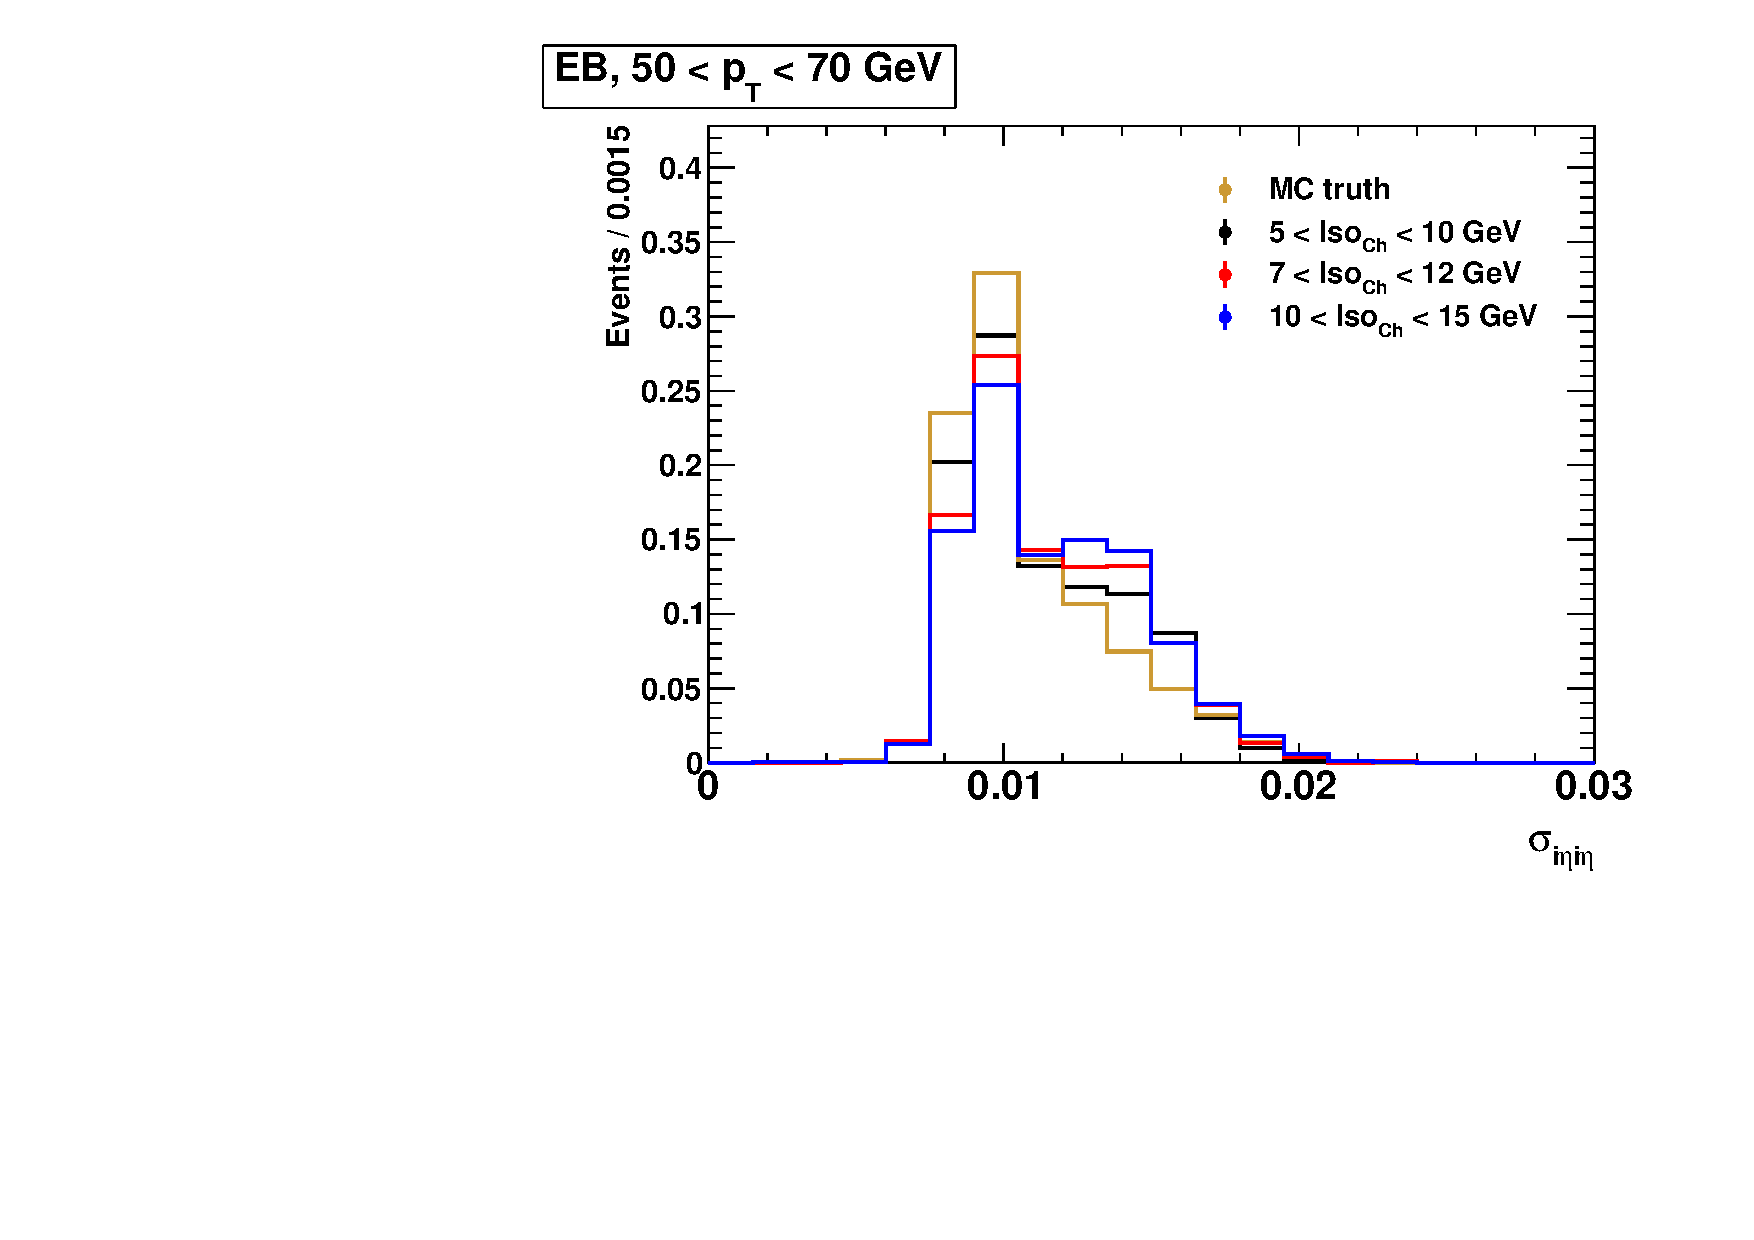
\includegraphics[scale=0.40]{figures/closure_test_fake_template_sieie_EB_pt50To70_sample_all.pdf}
  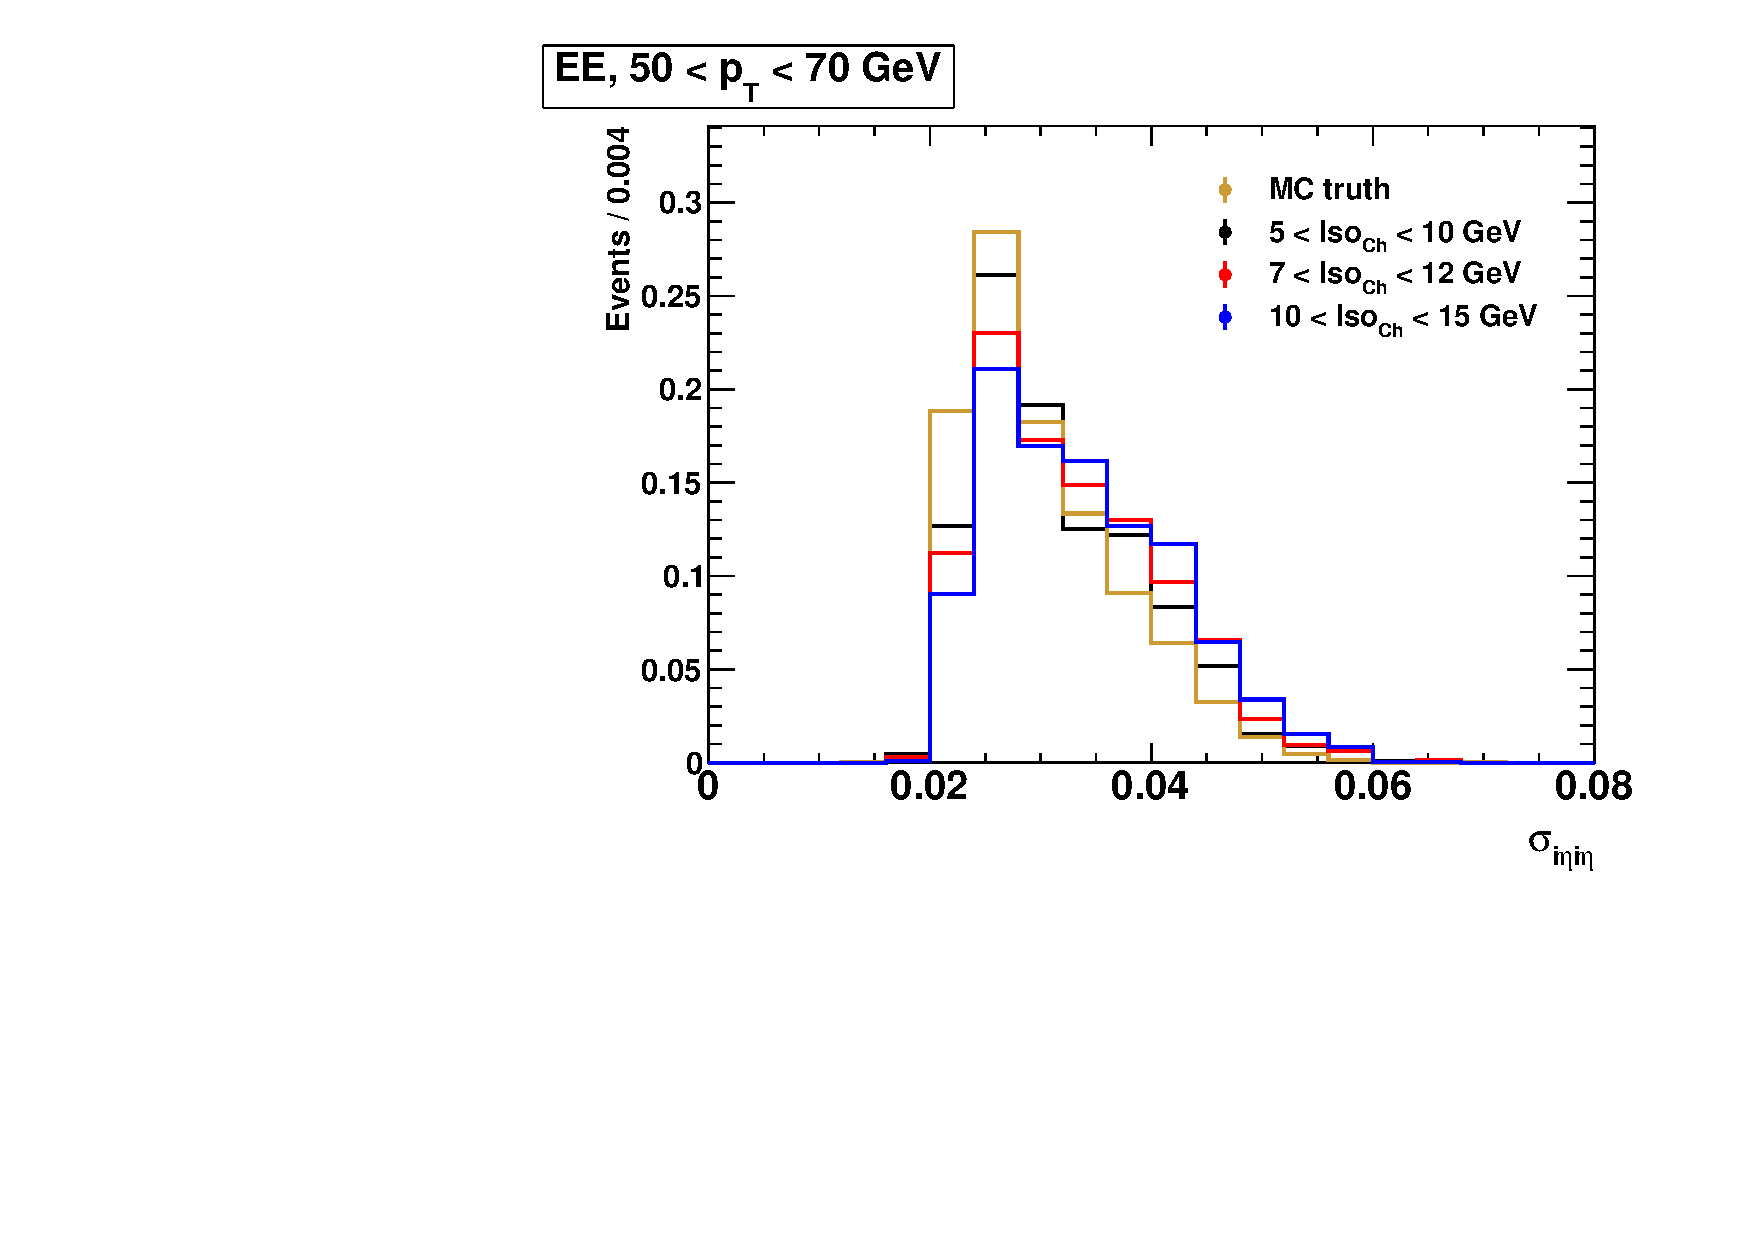
\includegraphics[scale=0.40]{figures/closure_test_fake_template_sieie_EE_pt50To70_sample_all.pdf}
  \caption{Fake templates extracted from the MC sample used in the fake rate closure test compared against the MC truth fake templates for $50 < \pt < 70\GeV$ in the EB (left) and EE (right). The template variable is \sieie.}
  \label{fig:mc_fake_templates_fixed_pt}
\end{figure}

We see that as the sideband definition is pushed further away from the region within the photon ID cut, the resulting template becomes more biased towards larger \sieie compared to the truth information. We choose our nominal sideband to have the selection of $5 < \chiso < 10\GeV$. Fig.~\ref{fig:mc_fake_templates_fixed_sideband} shows the \pt evolution of the these fake templates using the nominal \chiso sideband choice.

\begin{figure}[!htbp]
  \centering
  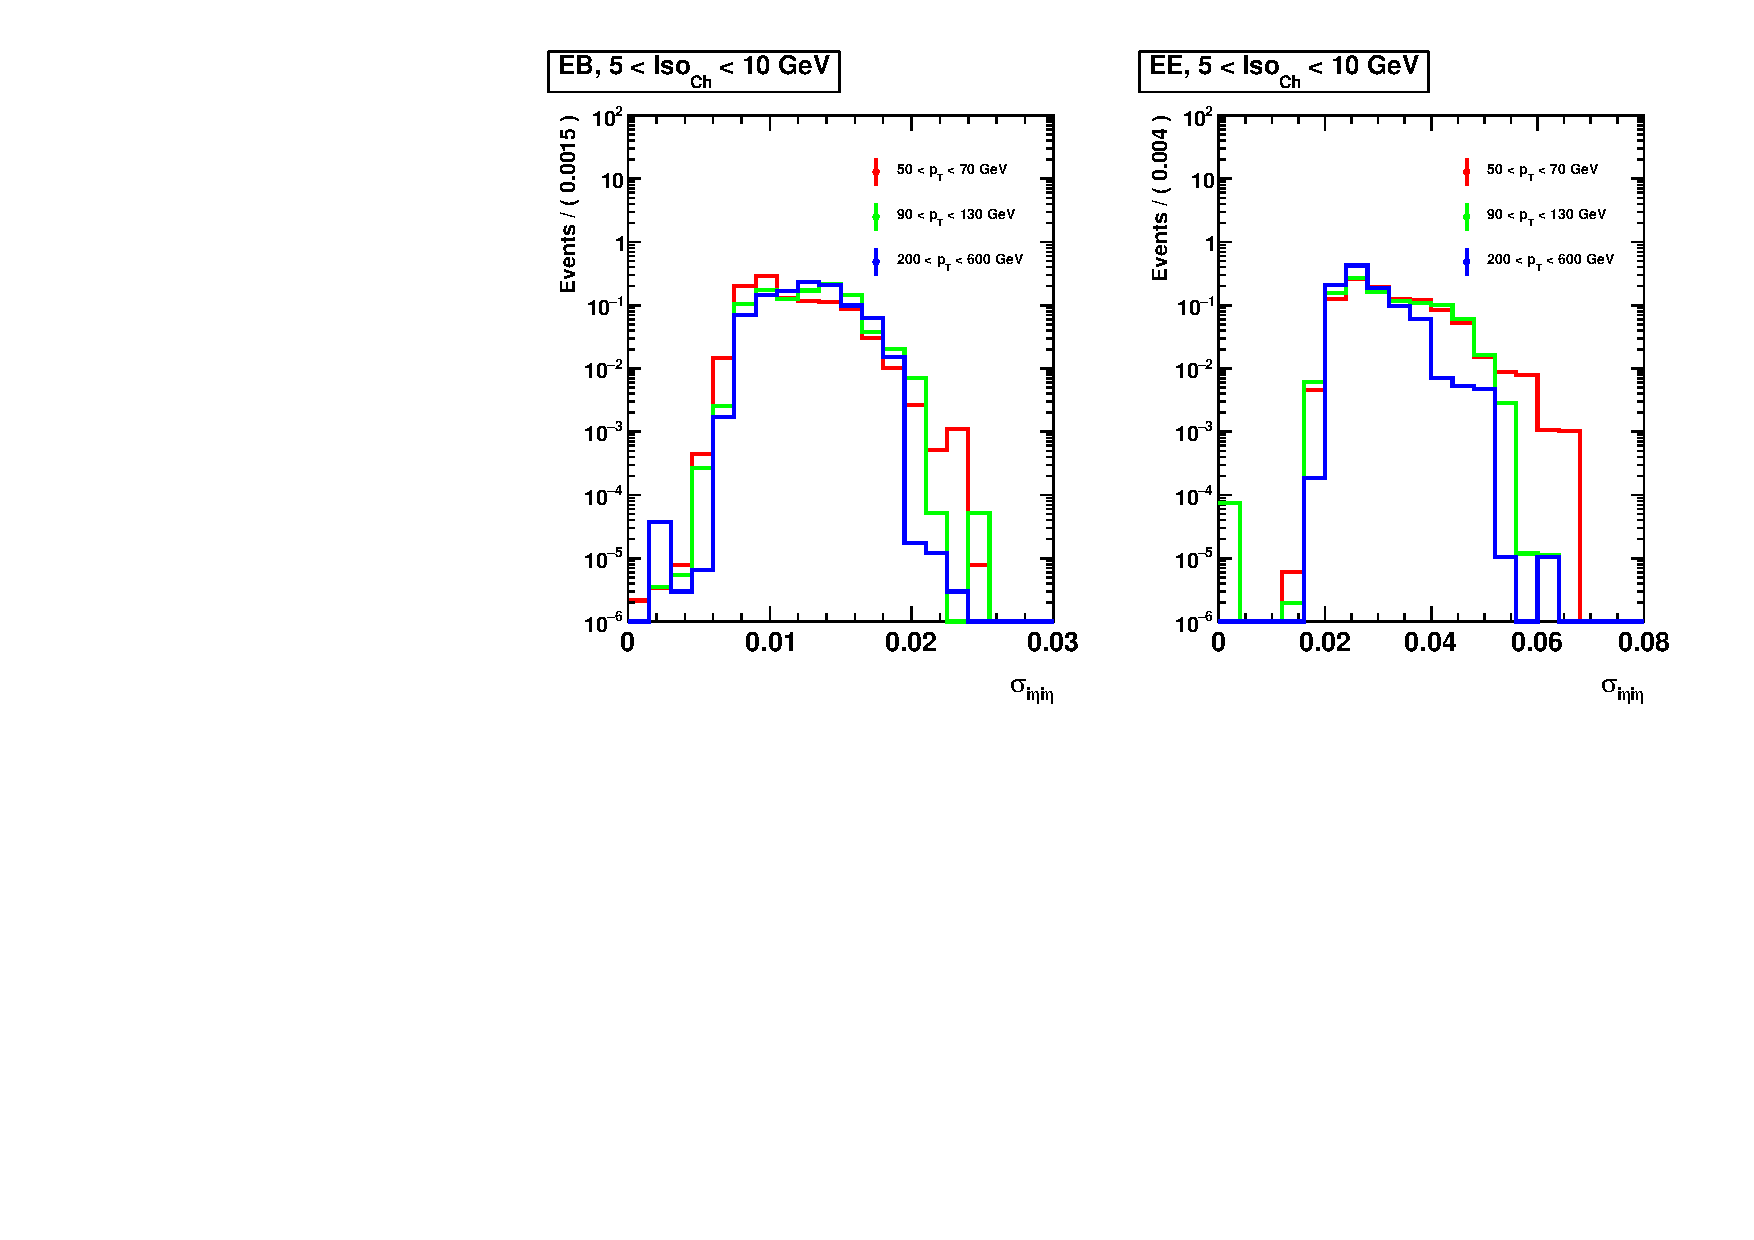
\includegraphics[scale=0.63]{figures/closure_test_fake_templates_sieie_overlaid_sample_all.pdf}
  \caption{Fake templates used in the MC based closure test showing their \pt evolution using the nominal \chiso sideband definition of 5-10\GeV in the EB (left) and EE (right) regions.}
  \label{fig:mc_fake_templates_fixed_sideband}
\end{figure}

We see from this study that the sideband-defined template does a reasonable job of replicating the truth template for known fakes. There is clearly some bias, as expected, but, unfortunately, some bias is unavoidable since fakes in a sideband are intrinsically different from fakes that pass the photon ID. This bias is limited but is the main source of systematic uncertainty on the fake rate method.


\subsubsection{Testing the Fit Method using Templates to Extract Fake Yields}

With the creation of the fake templates validated in the simulated sample, we can next test the fake prediction obtained by using these templates to fit to the numerator \sieie distribution. This fit uses the same real templates that are used in the data fake rate method, but using the different \pt binning. Fig.~\ref{fig:closure_test_real_templates} shows the real templates normalized to 1\fbinv in the EB and EE categories comparing different photon \pt bins. We see the higher \pt photons are more isolated.

\begin{figure}[!htbp]
  \centering
  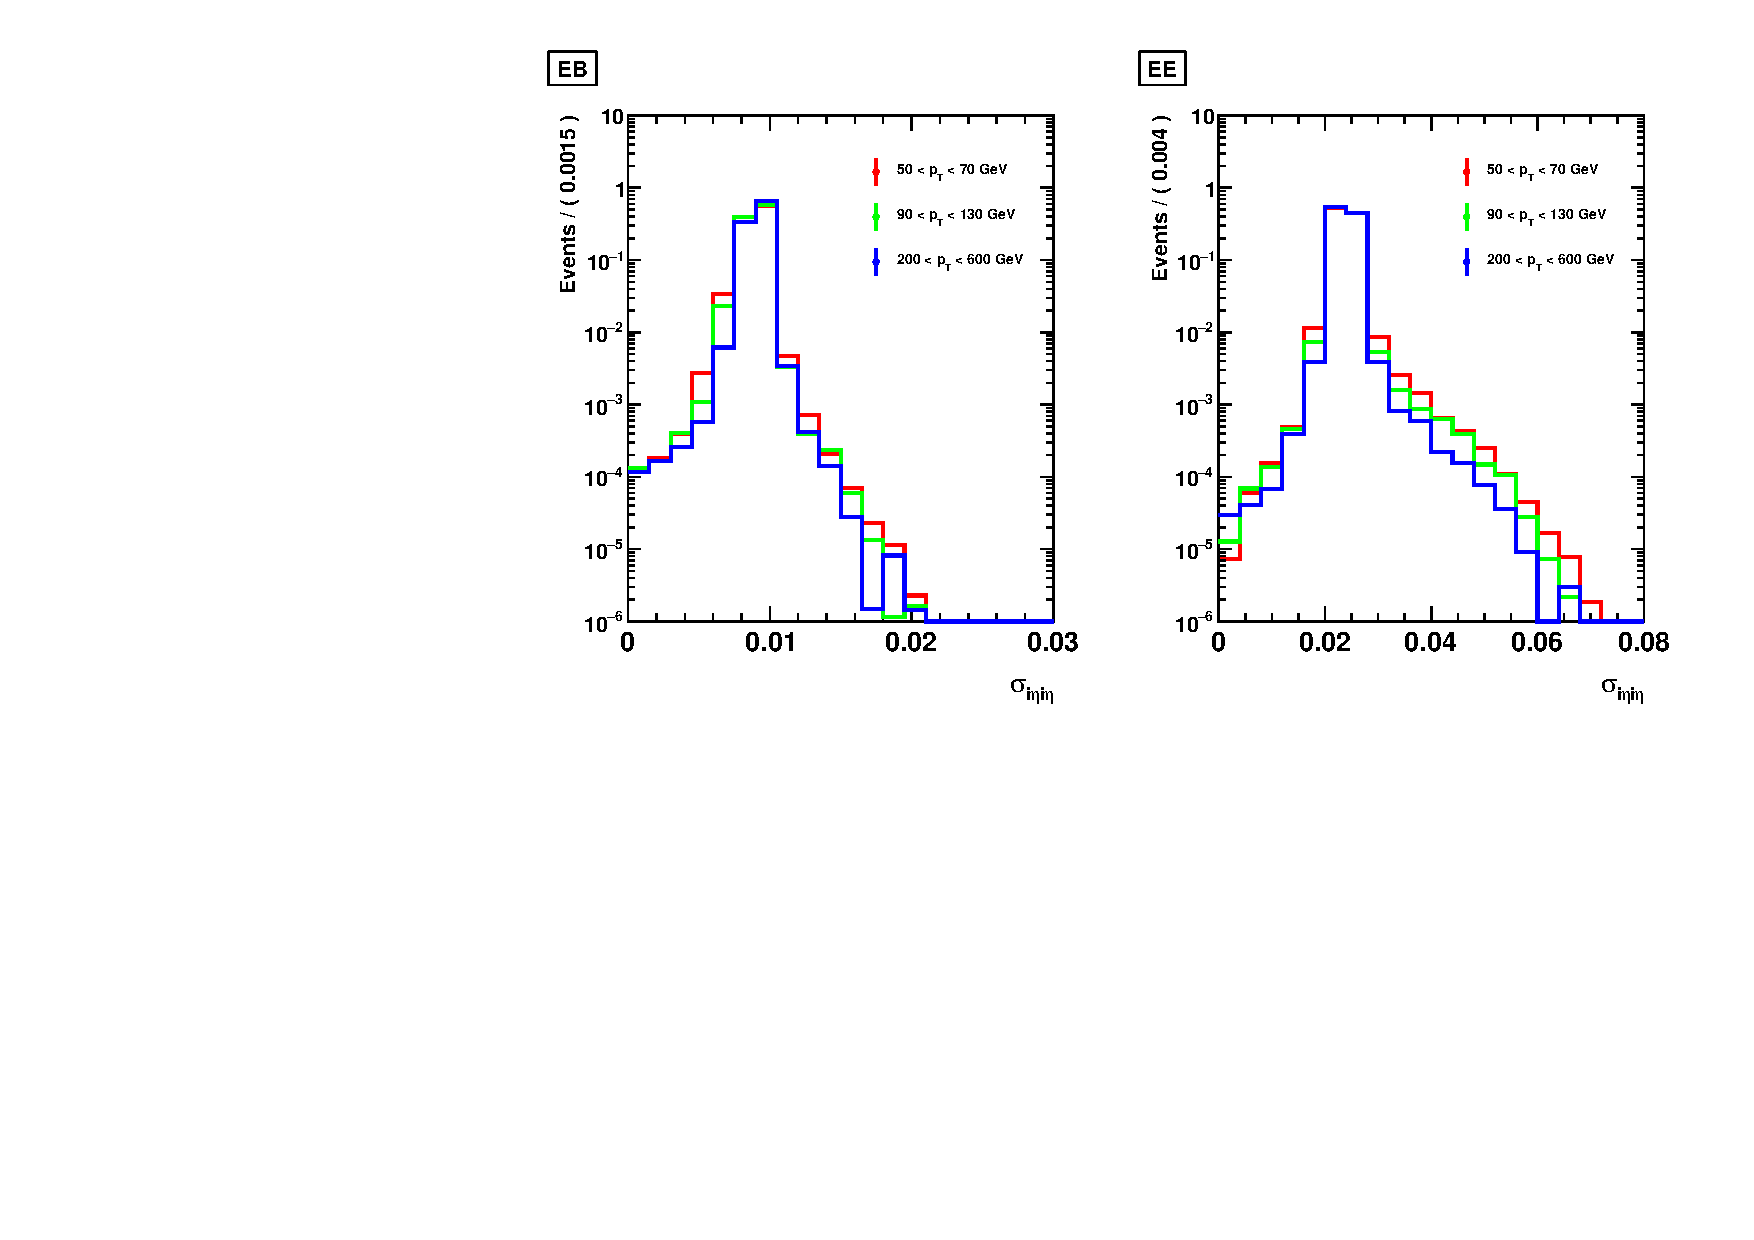
\includegraphics[scale=0.63]{figures/real_templates_sieie_overlaid_sample_all.pdf}
  \caption{Real templates using \sieie showing the evolution with photon \pt in the EB (left) and EE (right).}
  \label{fig:closure_test_real_templates}
\end{figure}

To better handle the lower statistics in the MC sample, the template fit is performed (in \sieie) using a negative log-likelihood function with errors calculated using the method by Barlow and Beeston~\cite{Barlow-Beeston:1993} incorporating an error term in the likelihood function. The fits are done for each \pt bin in the EB and EE separately. An example fit for photons in each category with $90 < \pt < 130\GeV$ is shown in Fig.~\ref{fig:closure_test_template_fit}. The fits for all \pt bins are given in Appendix~\ref{sec:mc_fake_rate_fits}.

\begin{figure}[!htbp]
  \centering
  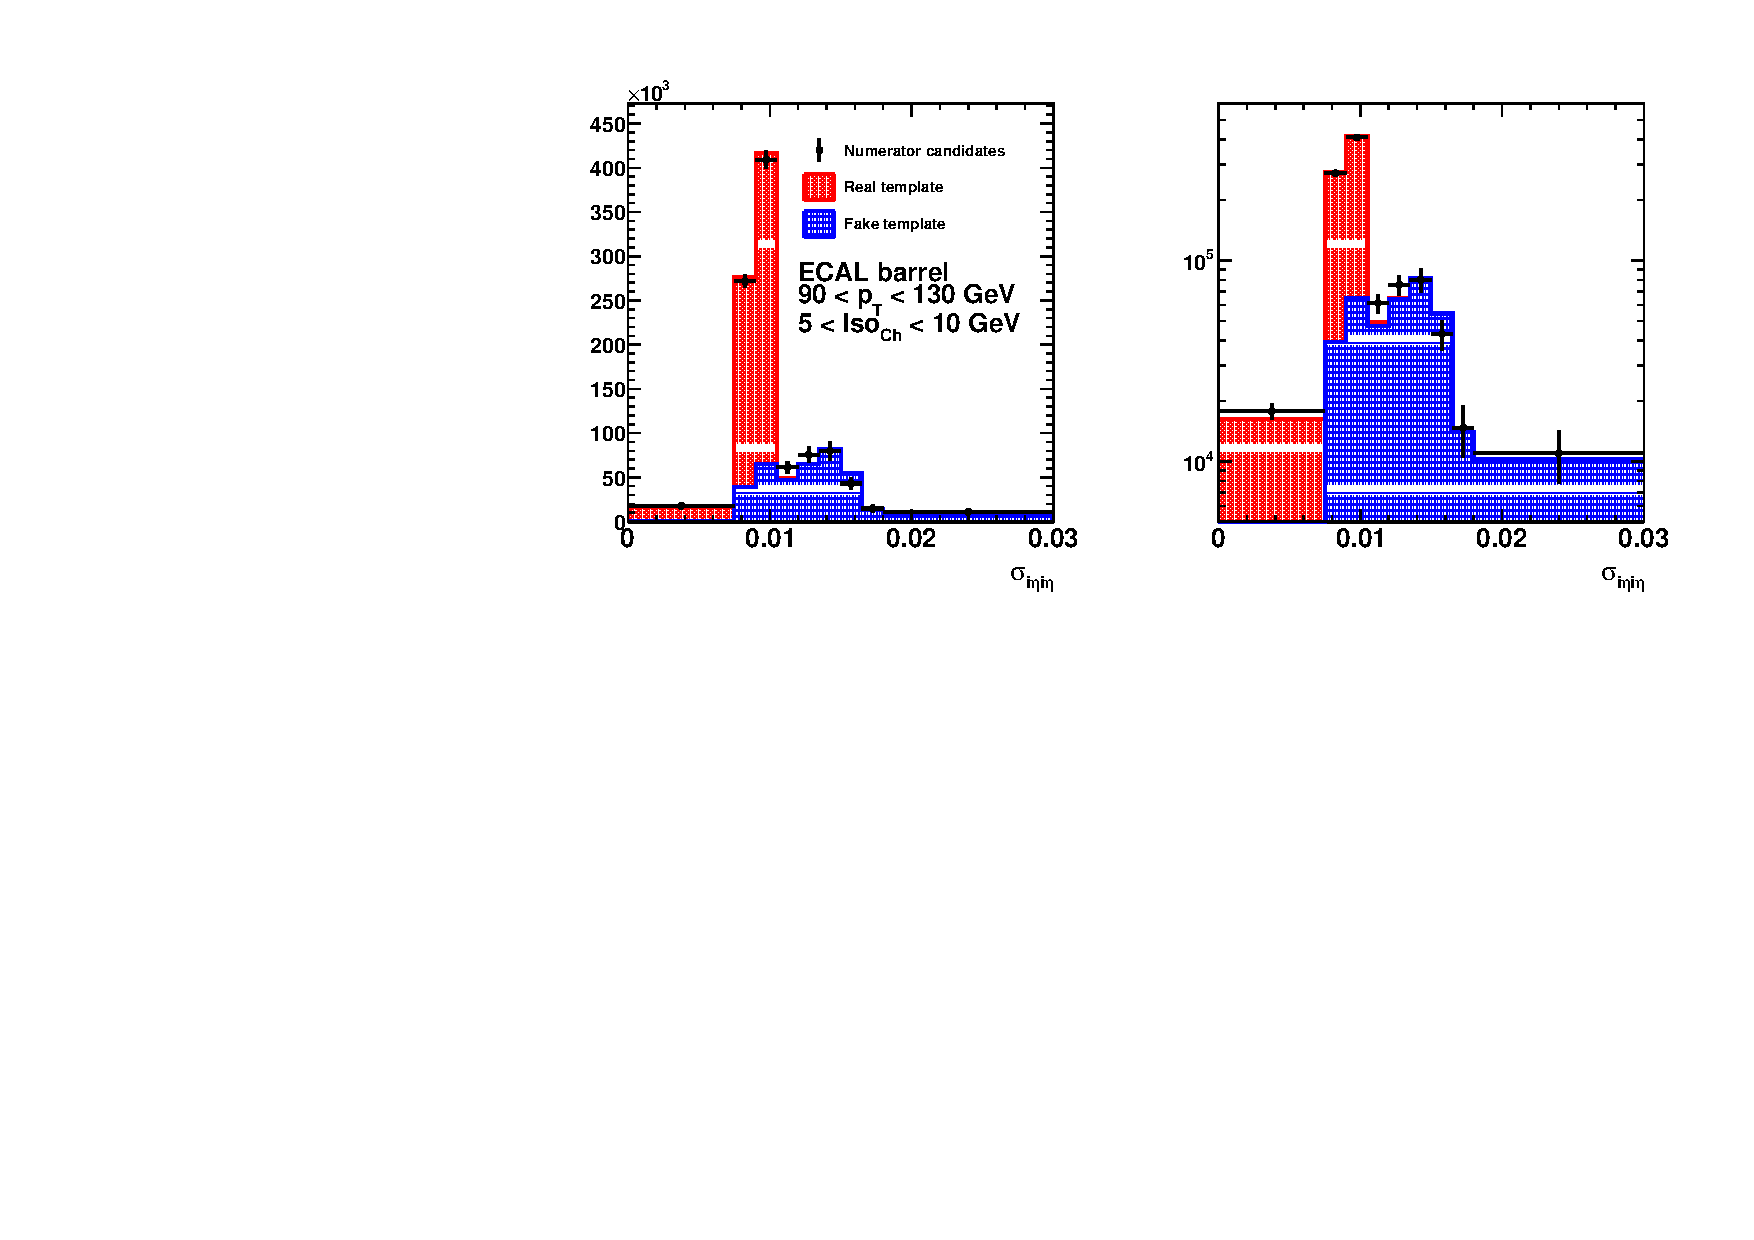
\includegraphics[scale=0.63]{figures/closure_test_h_pt90To130_chIso5To10_EB_Fake_sieie.pdf}
  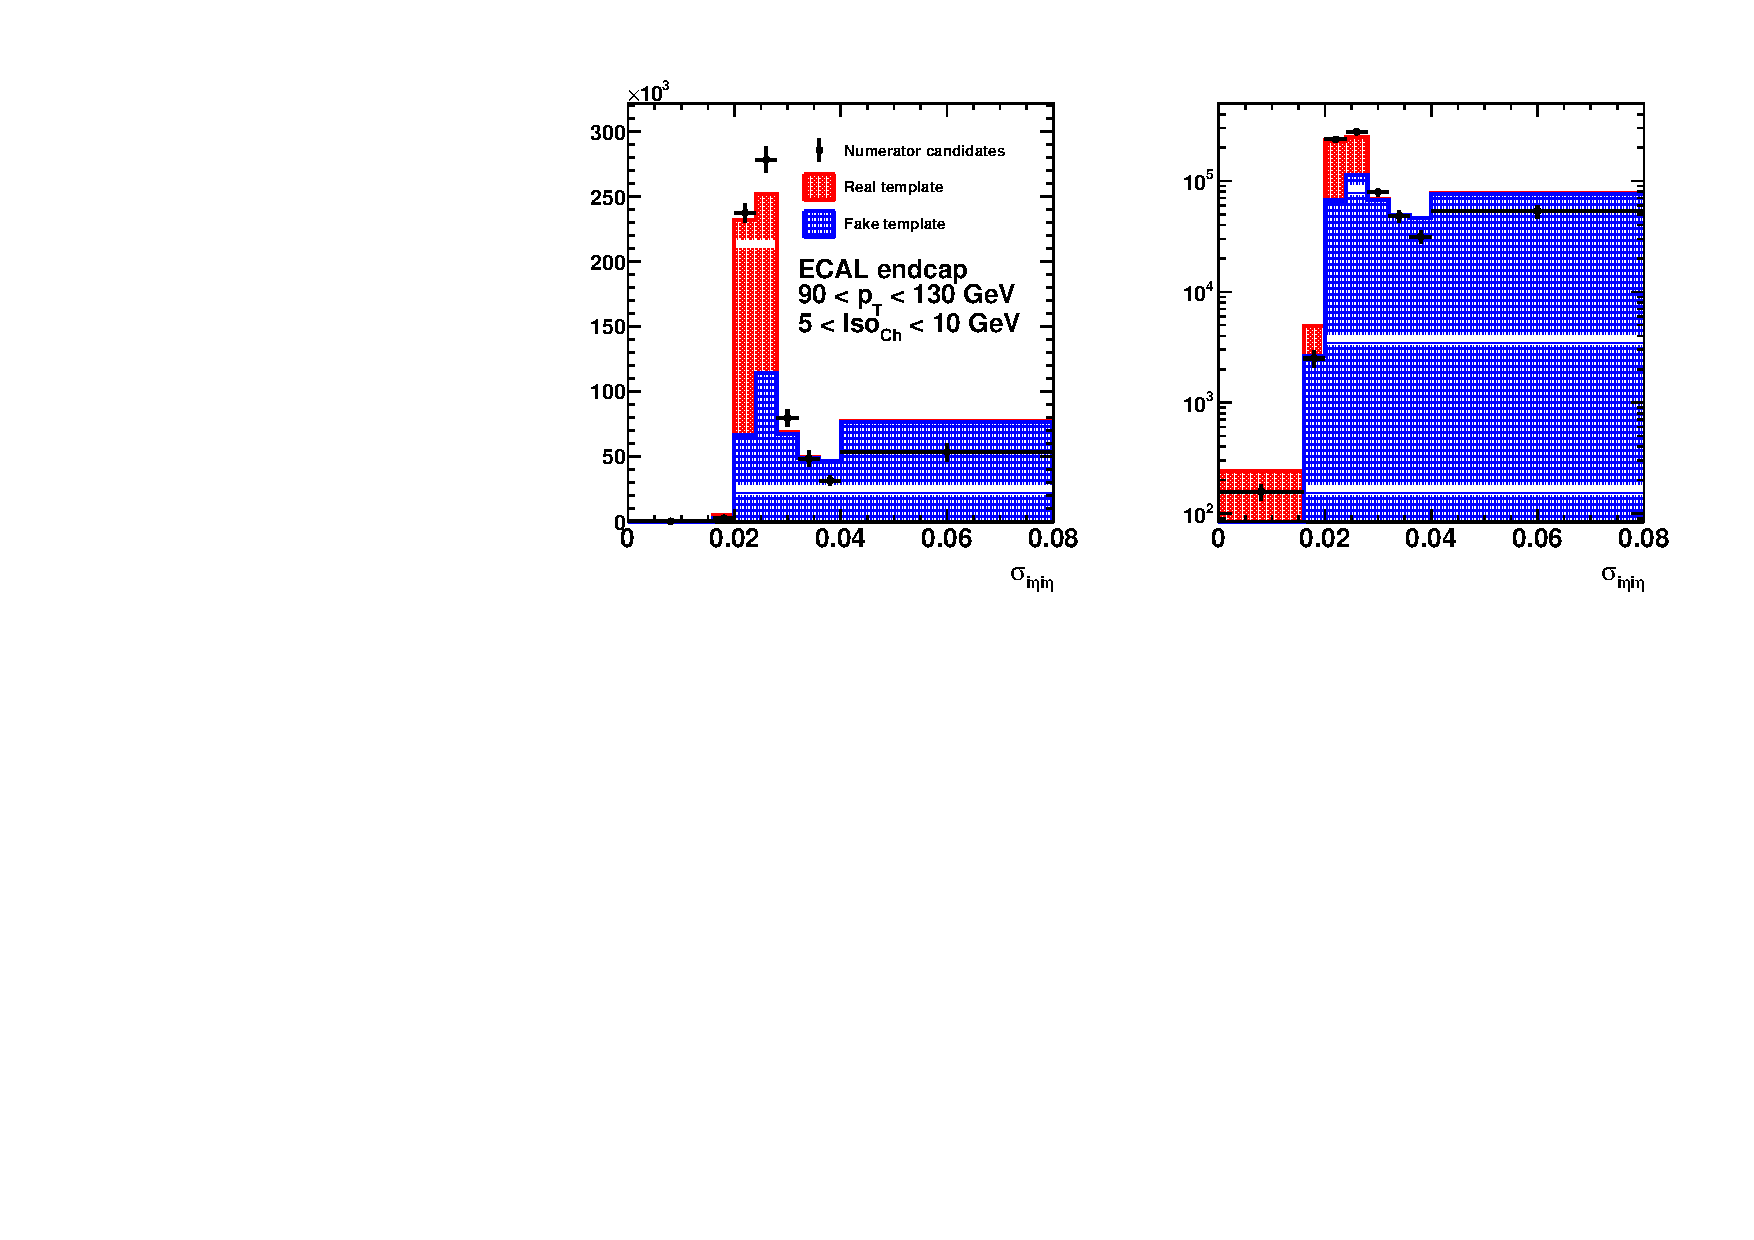
\includegraphics[scale=0.63]{figures/closure_test_h_pt90To130_chIso5To10_EE_Fake_sieie.pdf}
  \caption{Template fits using \sieie for the MC closure test with $90 < \pt < 130\GeV$ in the EB (top) and EE (bottom).}
  \label{fig:closure_test_template_fit}
\end{figure}

After the fit, the photon ID cut for \sieie is applied to the fake template and it is integrated in order to provide a fake prediction in each separate \pt bin. This is the numerator of the fake rate in the MC sample as a function of \pt. Dividing by the denominator extracted from the MC sample yields MC fake rate as a function of \pt. This procedure was repeated using fake templates constructed from sidebands with $7 < \chiso < 12\GeV$ and $10 < \chiso < 15\GeV$ in the MC sample. The three MC fake rates corresponding to all three different sideband choices are shown in Fig.~\ref{fig:closure_test_fake_rates_sieie}. In addition, since we have access to the MC truth information, we can simply count the number of fake photons in each \pt bin and divide by the same denominator to get an MC truth fake rate. This result is also shown in Fig.~\ref{fig:closure_test_fake_rates_sieie}. 

\begin{figure}[!htbp]
  \centering
  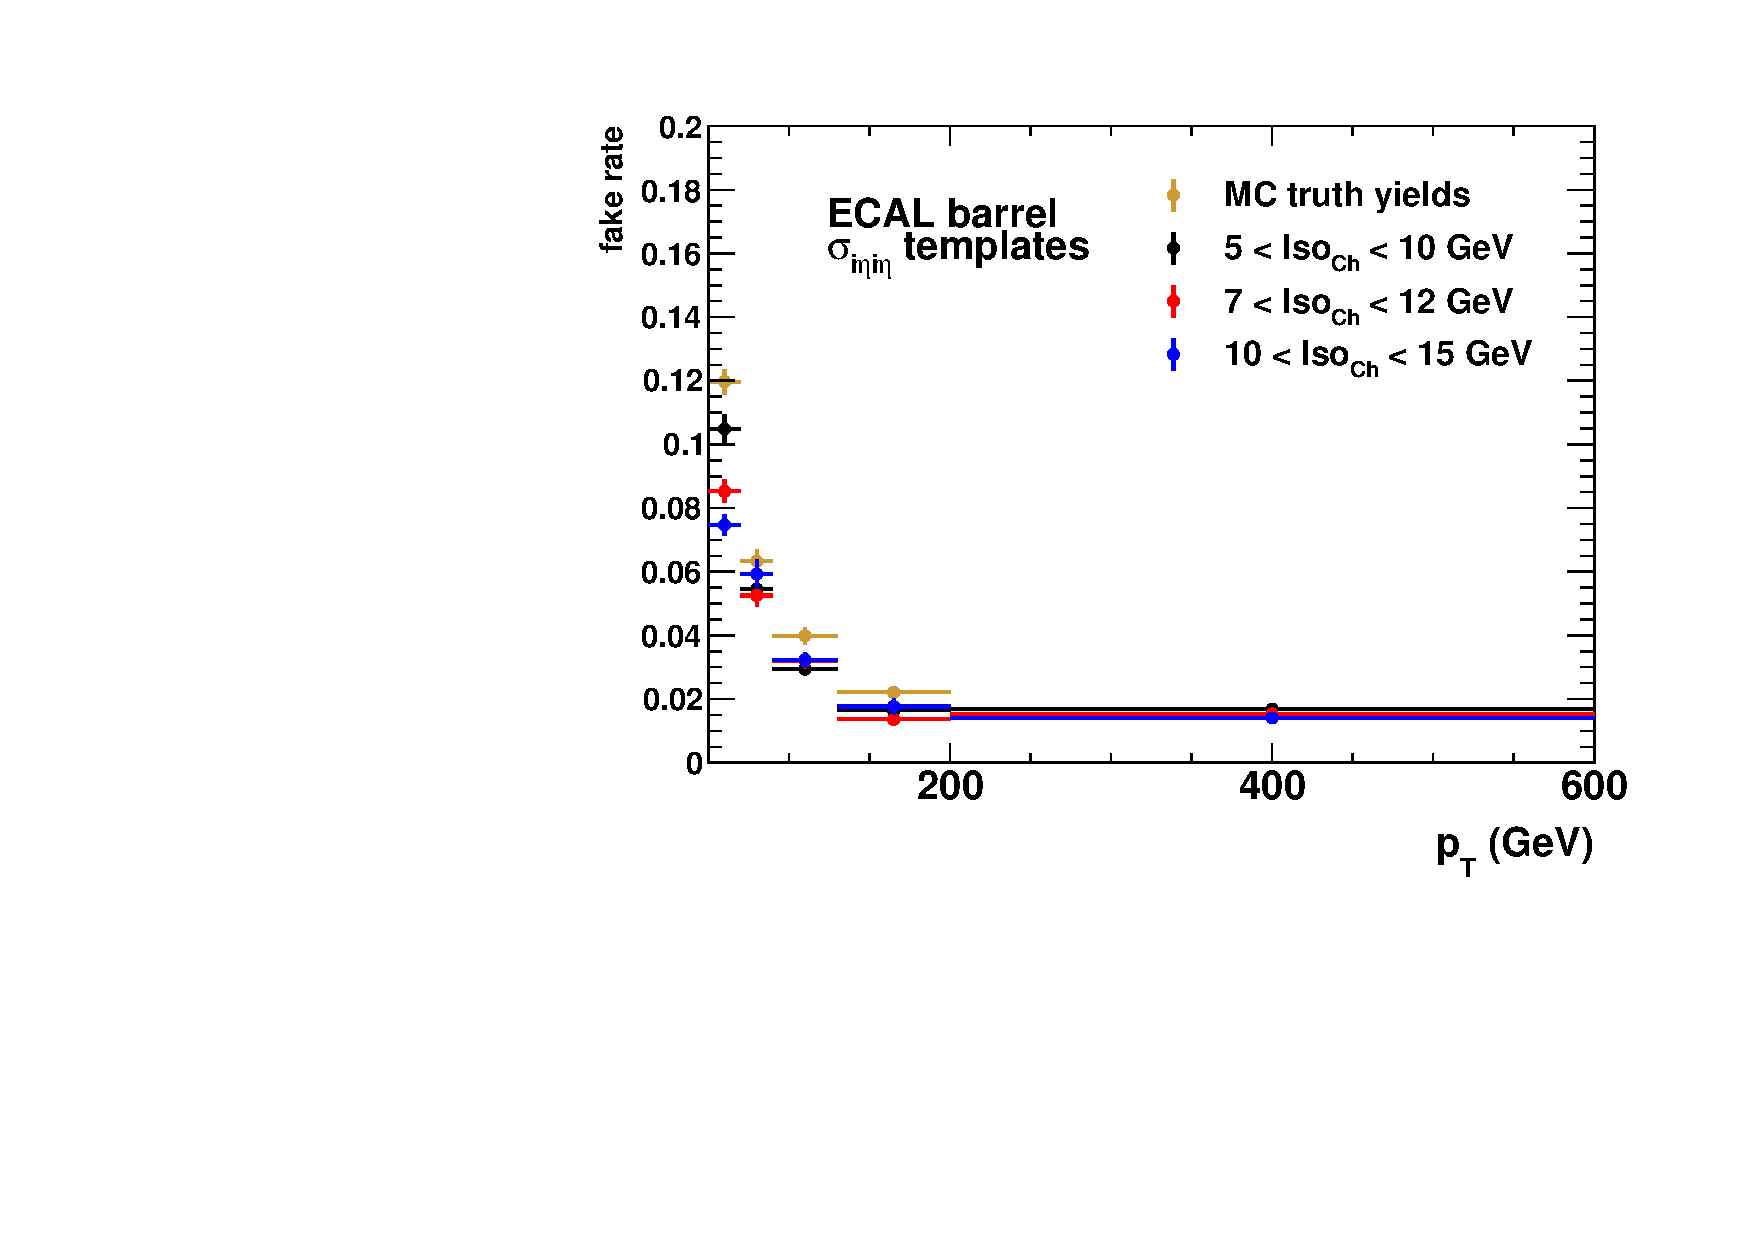
\includegraphics[scale=0.40]{figures/closure_test_fake_rates_sieie_EB.pdf}
  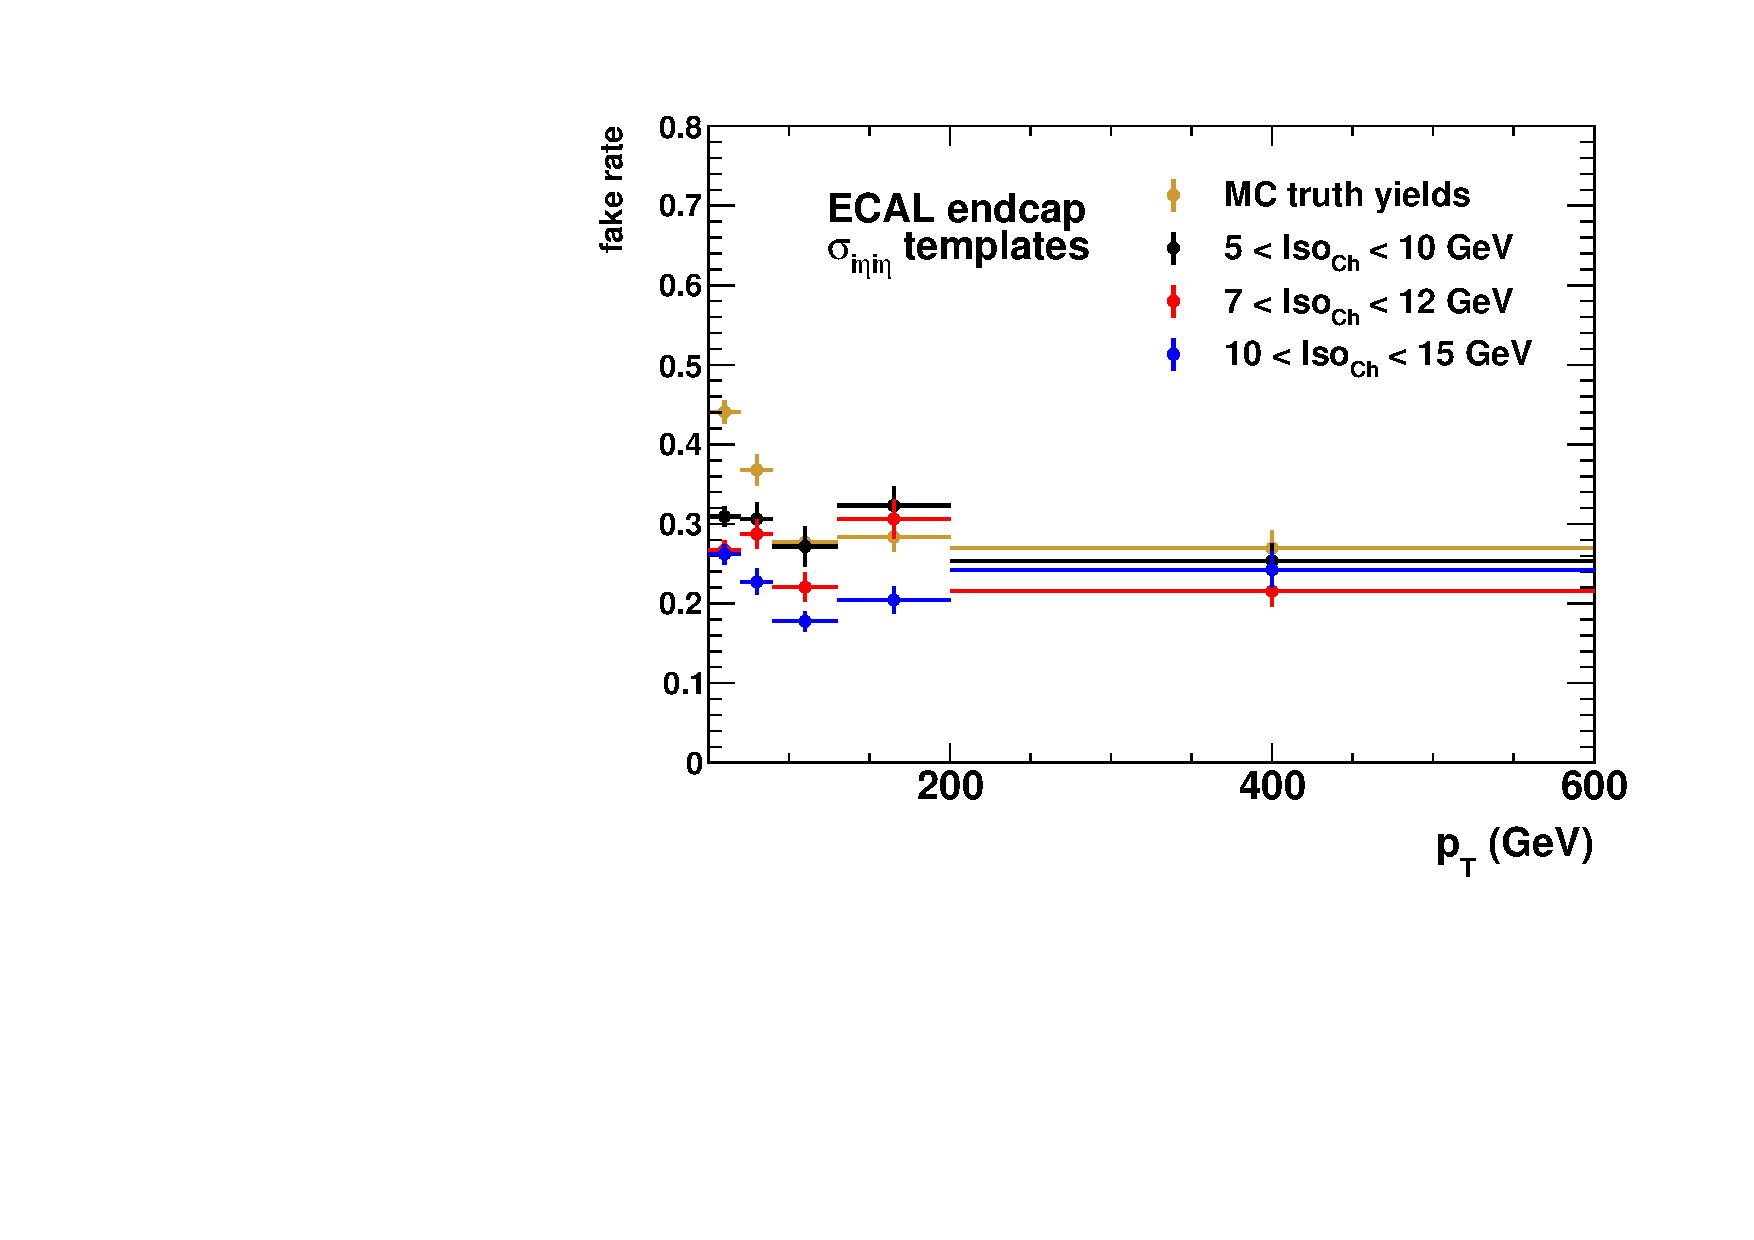
\includegraphics[scale=0.40]{figures/closure_test_fake_rates_sieie_EE.pdf}
  \caption{Fake rates for the MC closure test as a function of \pt using \sieie templates in the EB (left) and EE (right). Three different choices for the \chiso sidebands used in deriving the fake rates are compared against the fake rate using the MC truth information.}
  \label{fig:closure_test_fake_rates_sieie}
\end{figure}

We see that, in general, the template fit method somewhat underpredicts the actual number of fakes. This underprediction is attributed to the bias in the fake template constructed from the sideband definition, as seen above. We see that the underprediction is minimized by choosing a sideband in \chiso as close as possible to the photon ID region ($\chiso < 5\GeV$), as expected from the above study. We quantify the underprediction by calculating the ratio of the derived fake rate with the known MC truth fake rate as a function of \pt. This ratio is shown in Fig.~\ref{fig:closure_test_yields} using our nominal \chiso sideband for the MC fake rate prediction. In general, we observe an underprediction within an uncertainty of about 30\%, a degree of nonclosure consistent with this method based on its use in previous CMS analyses, such as in Ref.~\cite{CMS-PAS-EXO-12-045}.

\begin{figure}[!htbp]
  \centering
  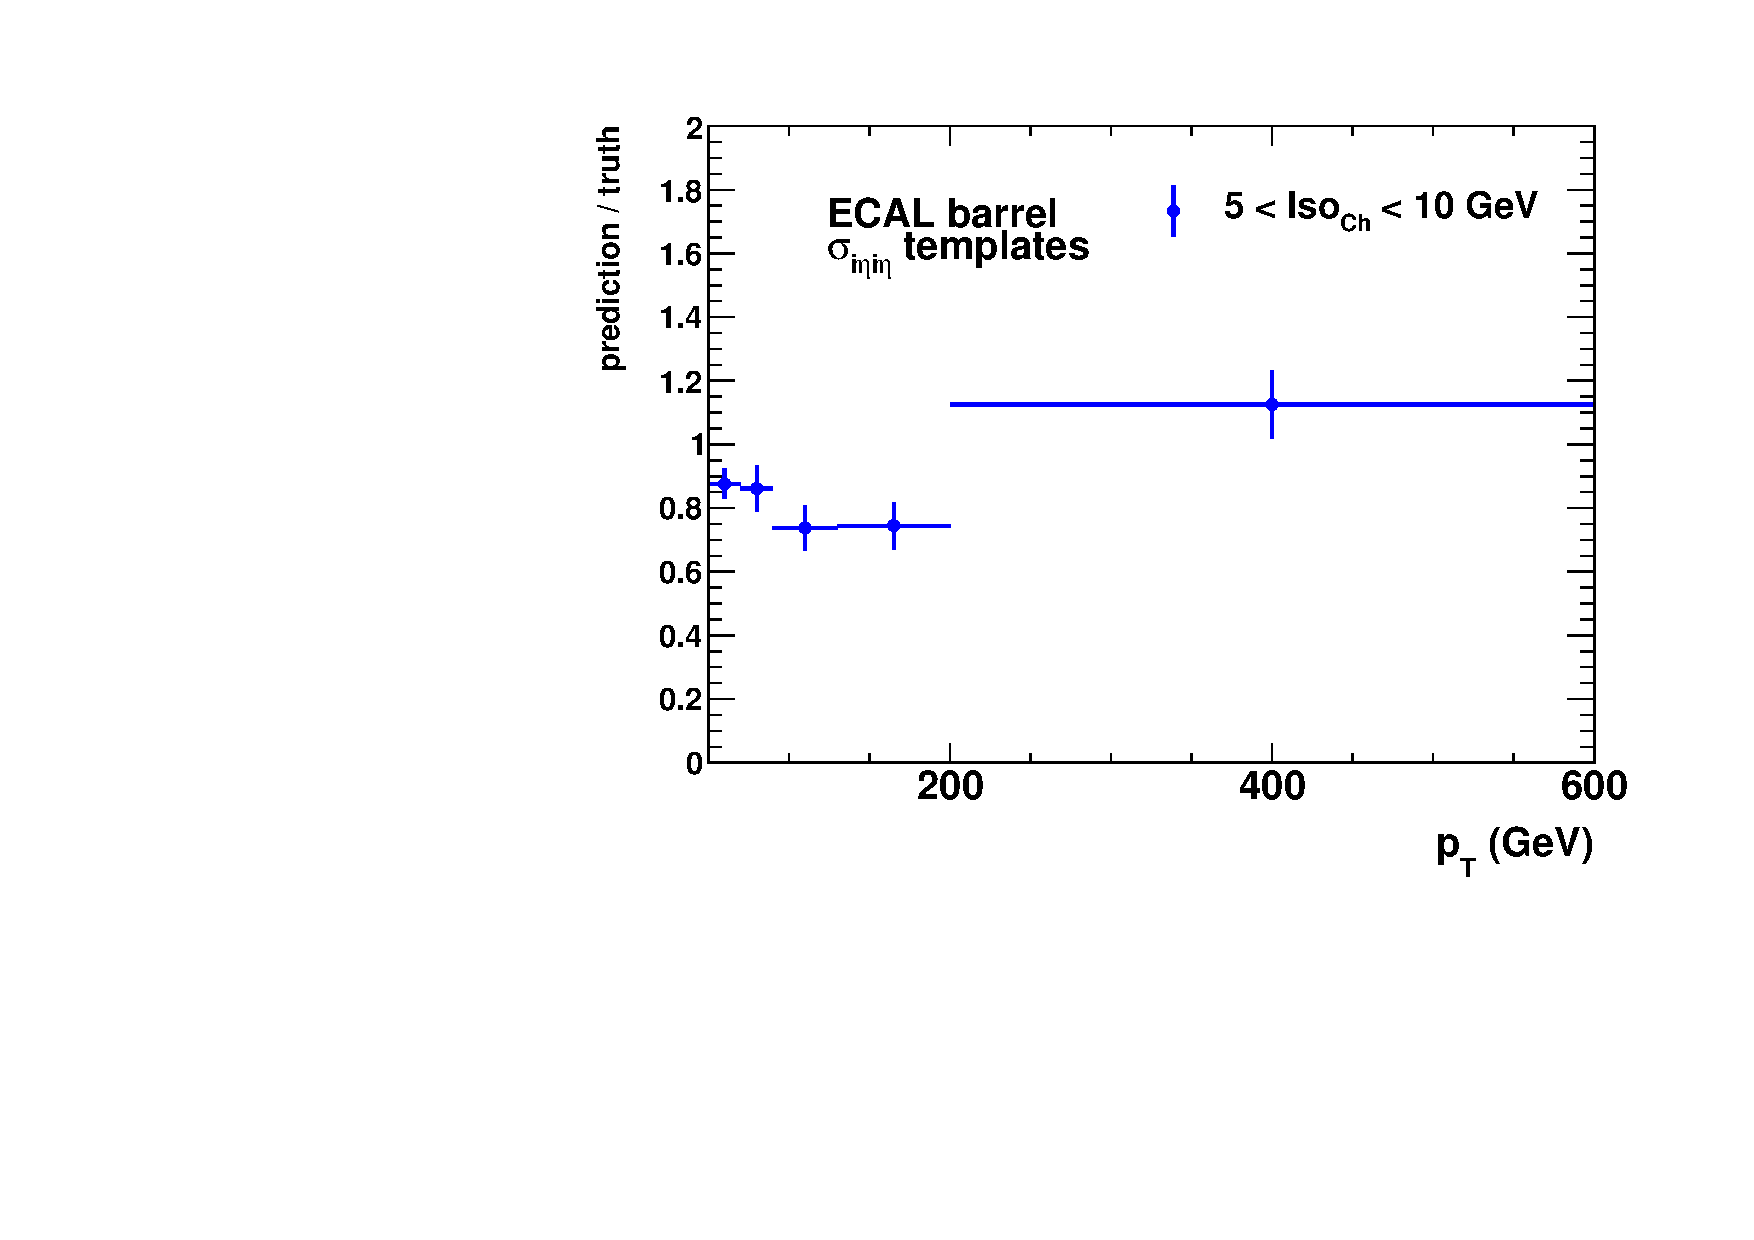
\includegraphics[scale=0.40]{figures/closure_test_fake_rate_ratio_sieie_EB.pdf}
  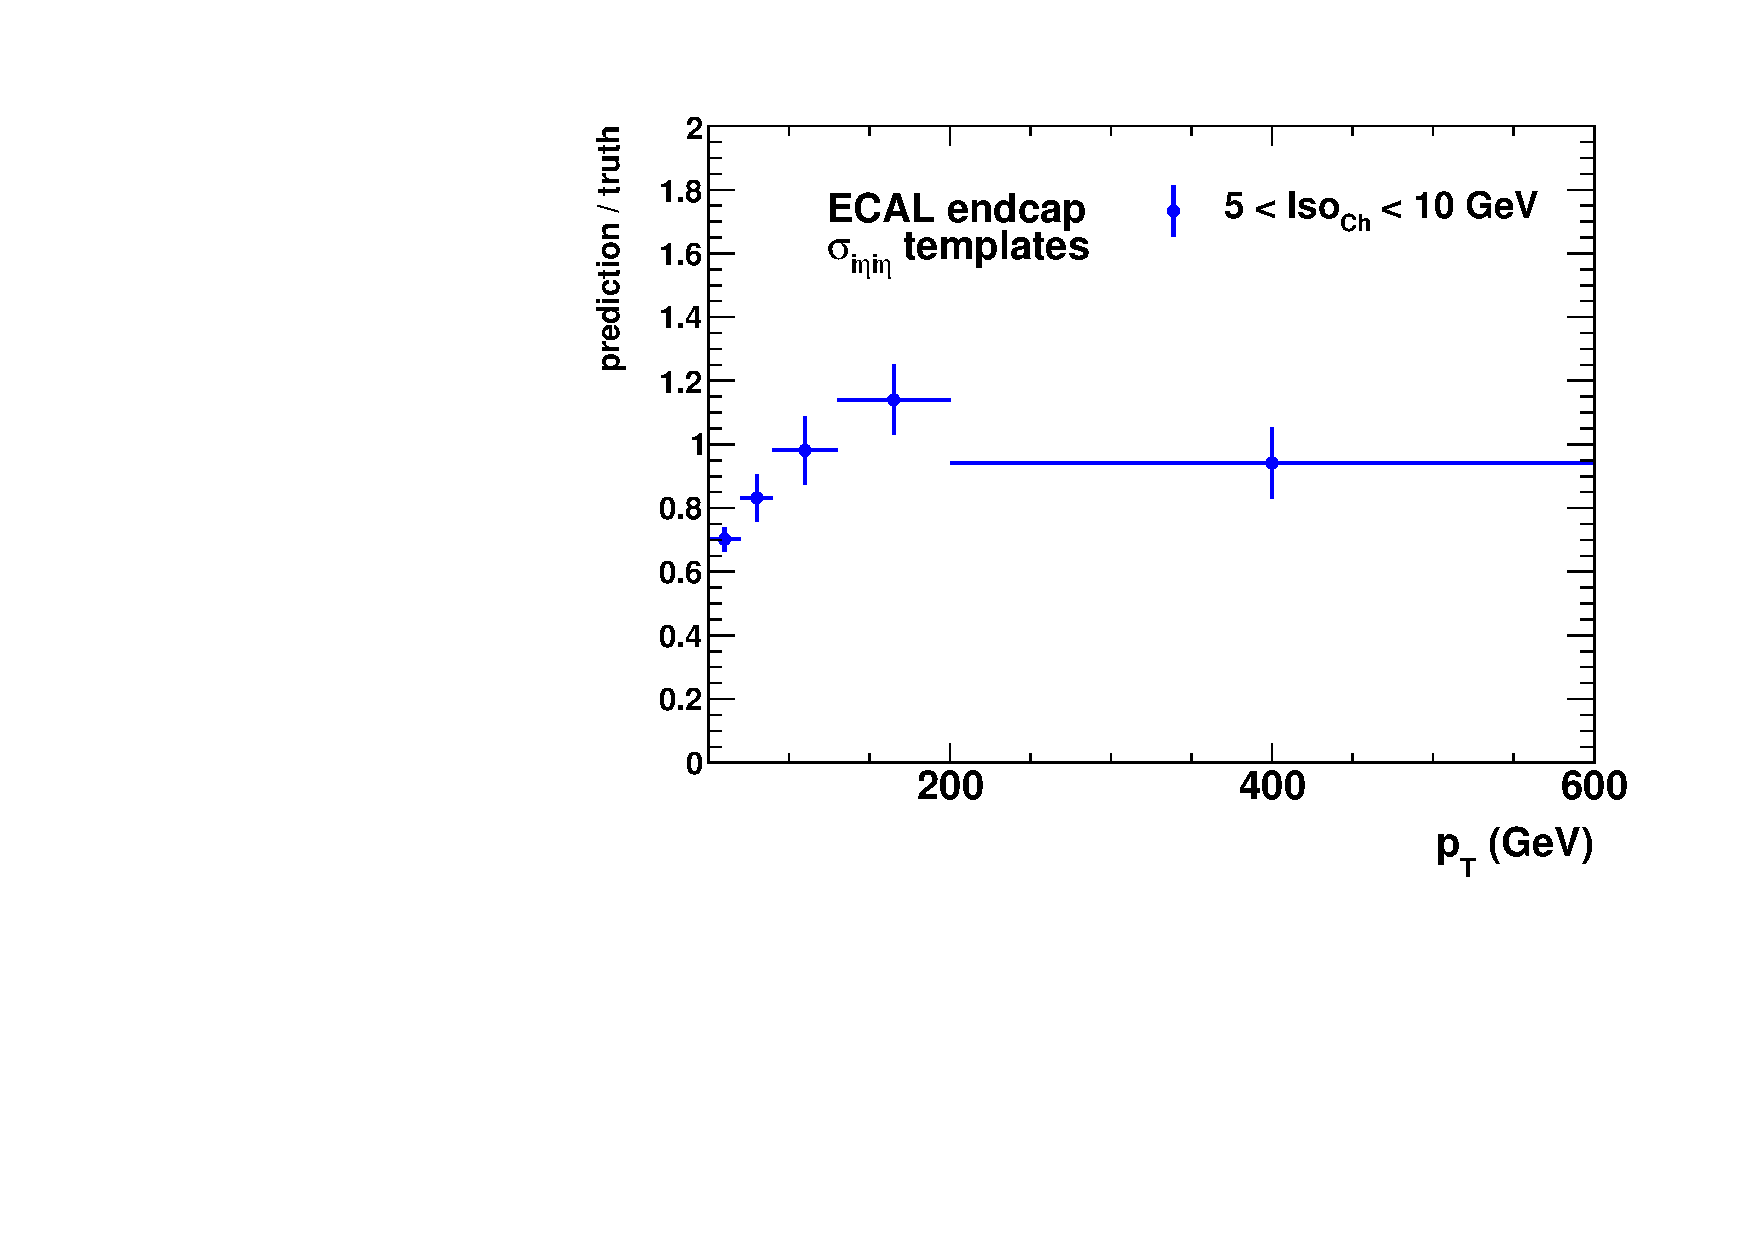
\includegraphics[scale=0.40]{figures/closure_test_fake_rate_ratio_sieie_EE.pdf}
  \caption{Comparison of the ratio of the fake yields obtained from the MC fake prediction using \sieie templates over the yields identified by the MC truth information in the EB (left) and EE (right) regions.}
  \label{fig:closure_test_yields}
\end{figure}

An alternative way of obtaining the MC truth fake rate is to use the MC truth information to derive the fake templates and then use them in the fitting procedure to produce the fake rate. This alternative procedure was performed and an example template fit using these fake templates in the bin $70 < \pt < 90\GeV$ is shown in Fig.~\ref{fig:closure_test_truth_template_fit}, separately for the EB and EE regions. The corresponding fake rates are shown in Fig.~\ref{fig:closure_test_fake_rates_sieie_truth}. These fake rates are in good agreement with those obtained using the MC truth yields, previously presented in Fig.~\ref{fig:closure_test_fake_rates_sieie}, helping to validate the fitting procedure.

\begin{figure}[!htbp]
  \centering
  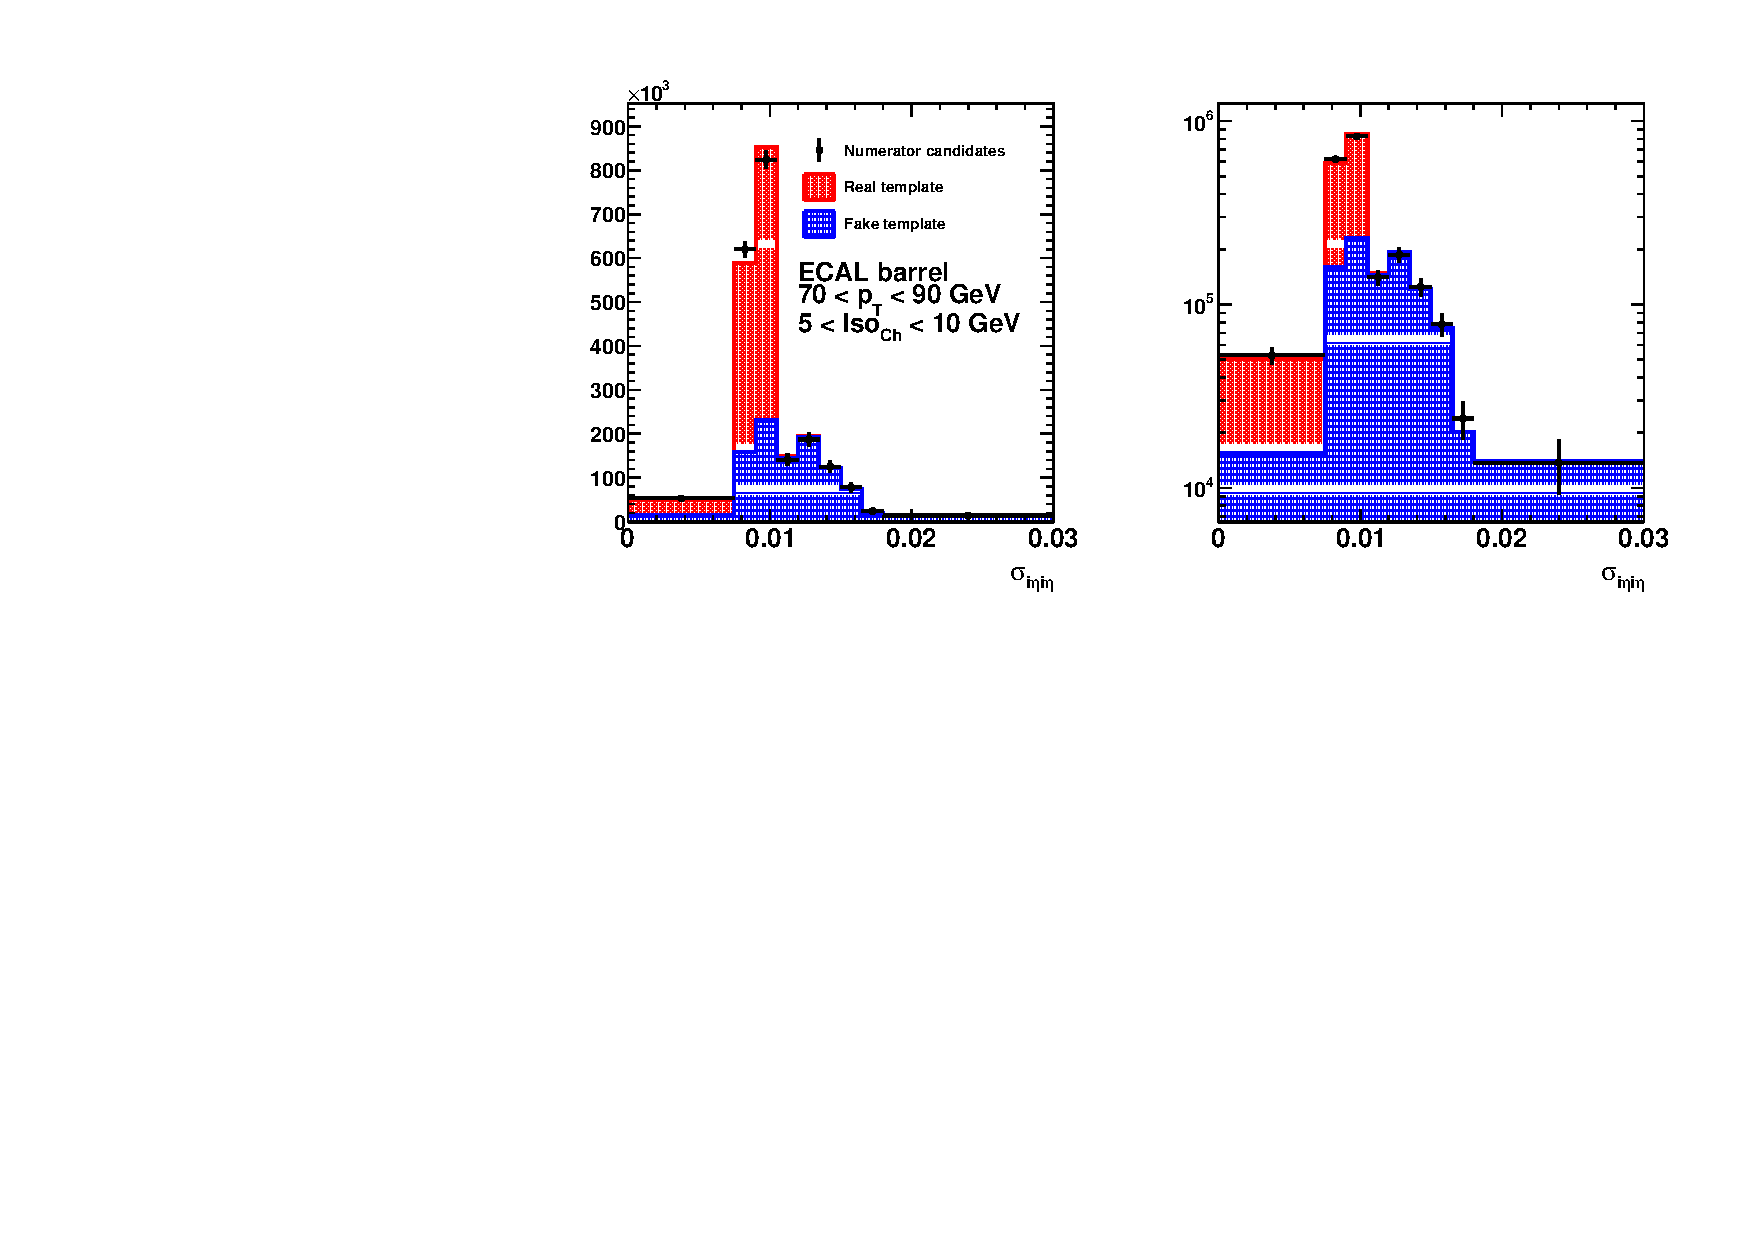
\includegraphics[scale=0.63]{figures/closure_test_h_pt70To90_chIso5To10_EB_Truth_sieie.pdf}
  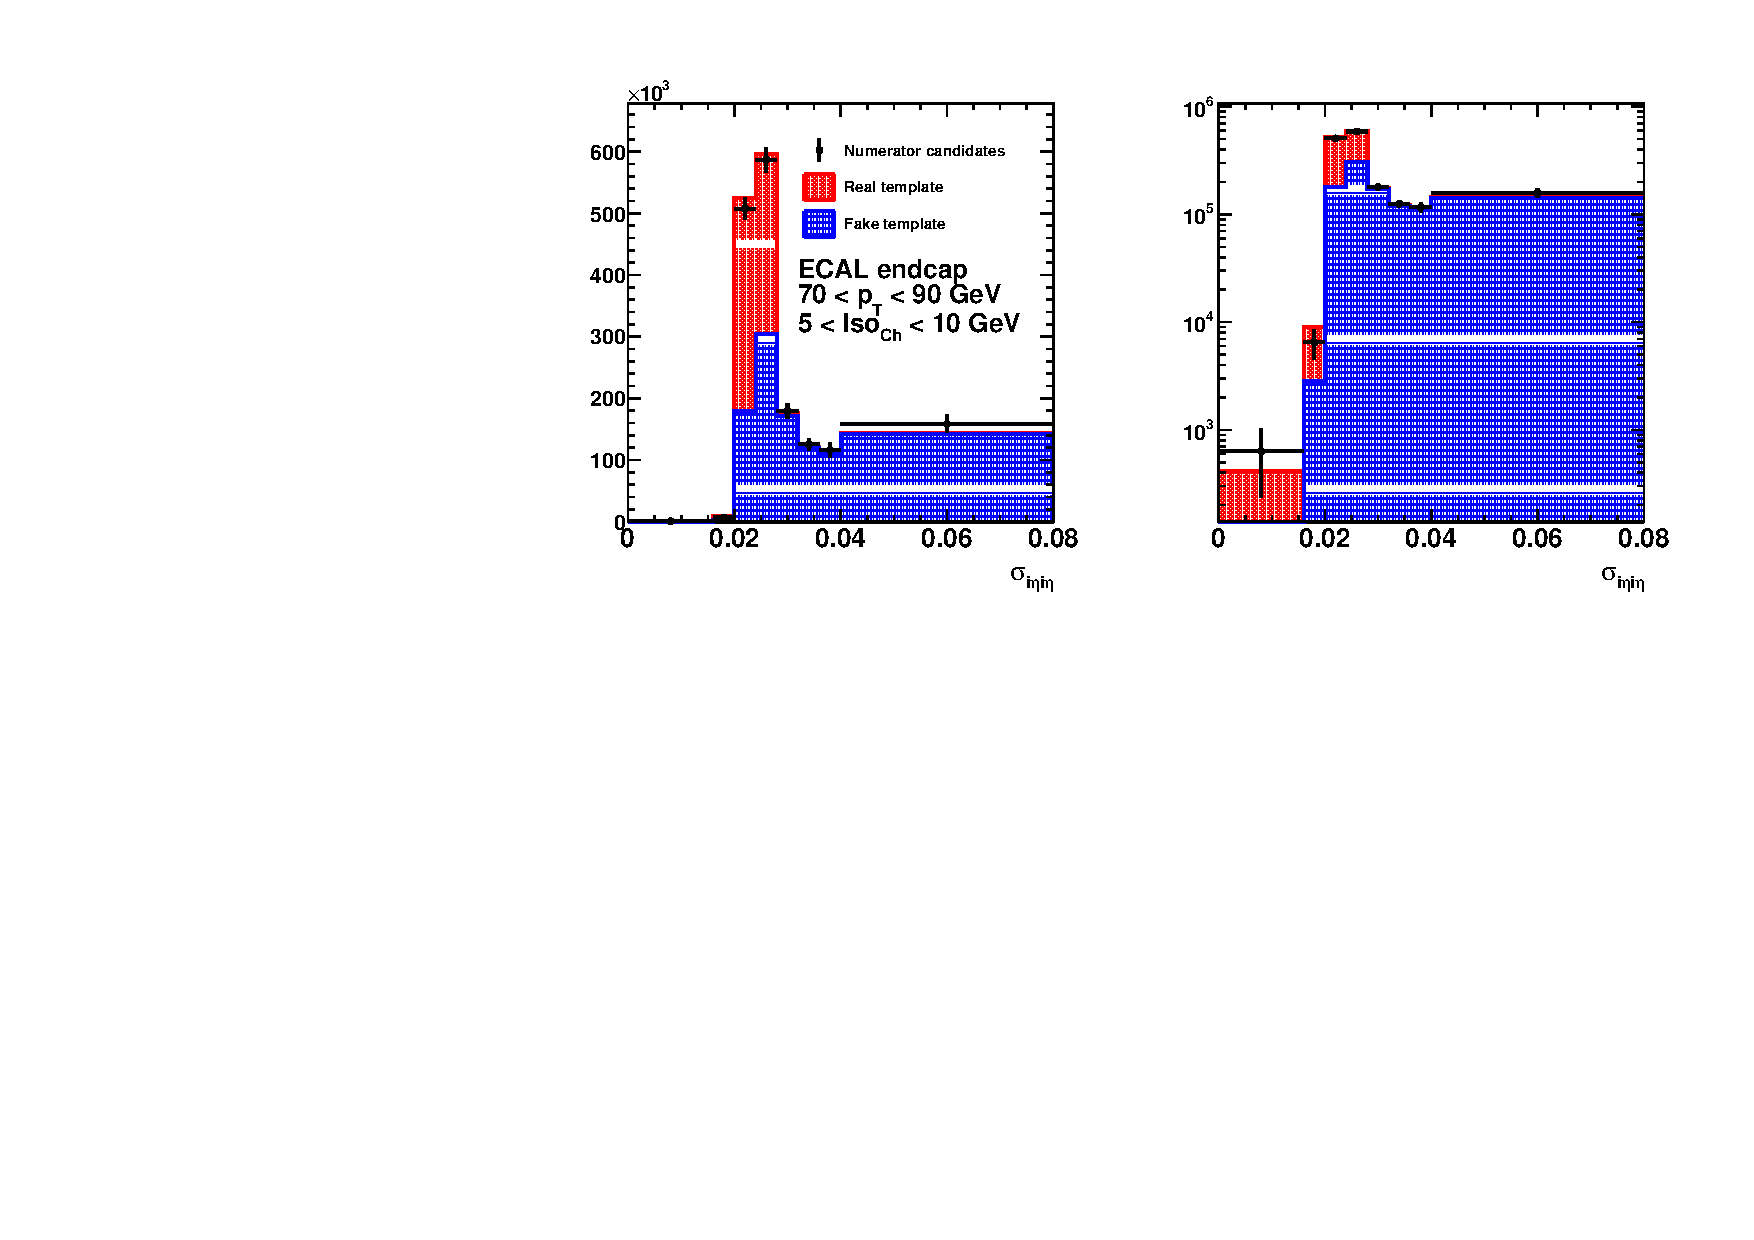
\includegraphics[scale=0.63]{figures/closure_test_h_pt70To90_chIso5To10_EE_Truth_sieie.pdf}
  \caption{Template fits using \sieie with fake templates derived using the MC truth information in the simulated sample with the nominal sideband definition for $70 < \pt < 90\GeV$ in the EB (top) and EE (bottom) regions.}
  \label{fig:closure_test_truth_template_fit}
\end{figure}

\begin{figure}[!htbp]
  \centering
  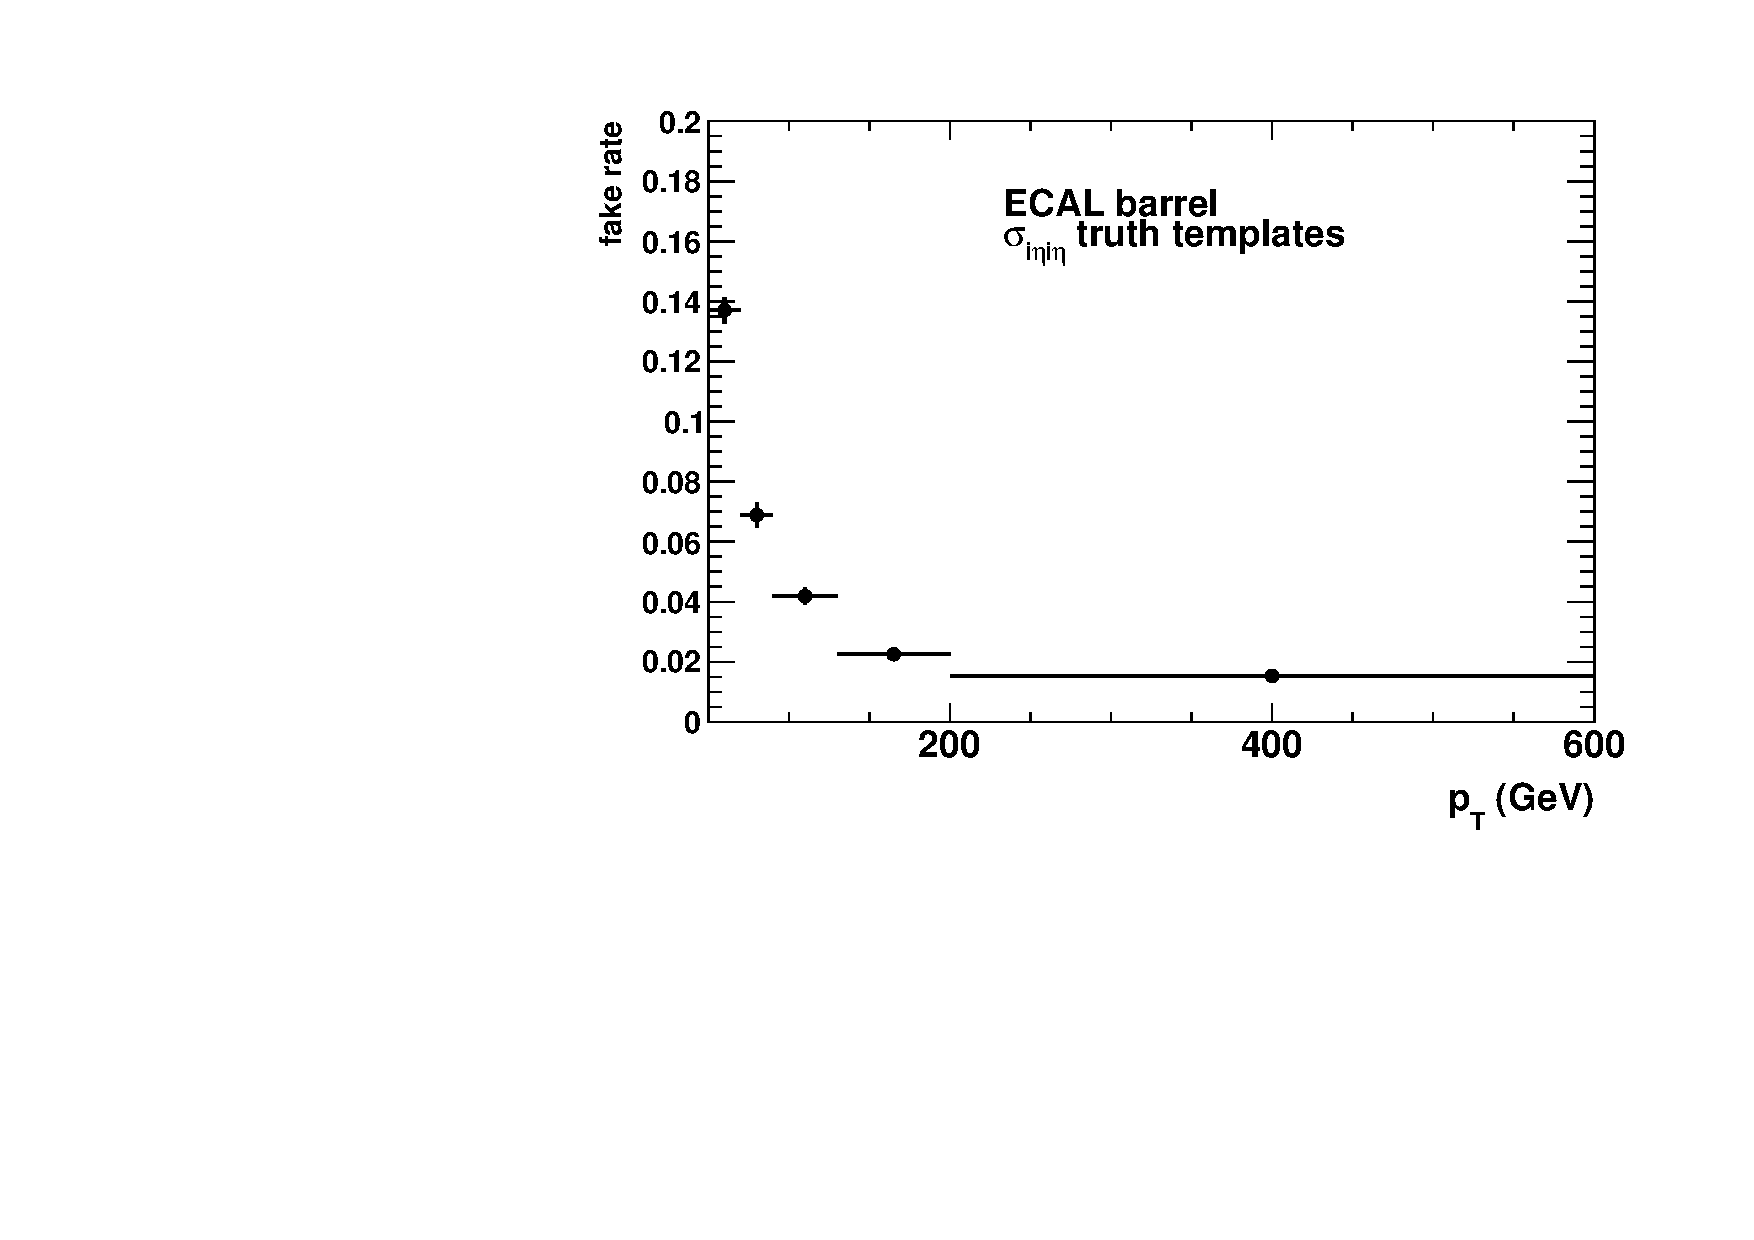
\includegraphics[scale=0.40]{figures/closure_test_EBTruthFakeRate_sieie_chIso5To10.pdf}
  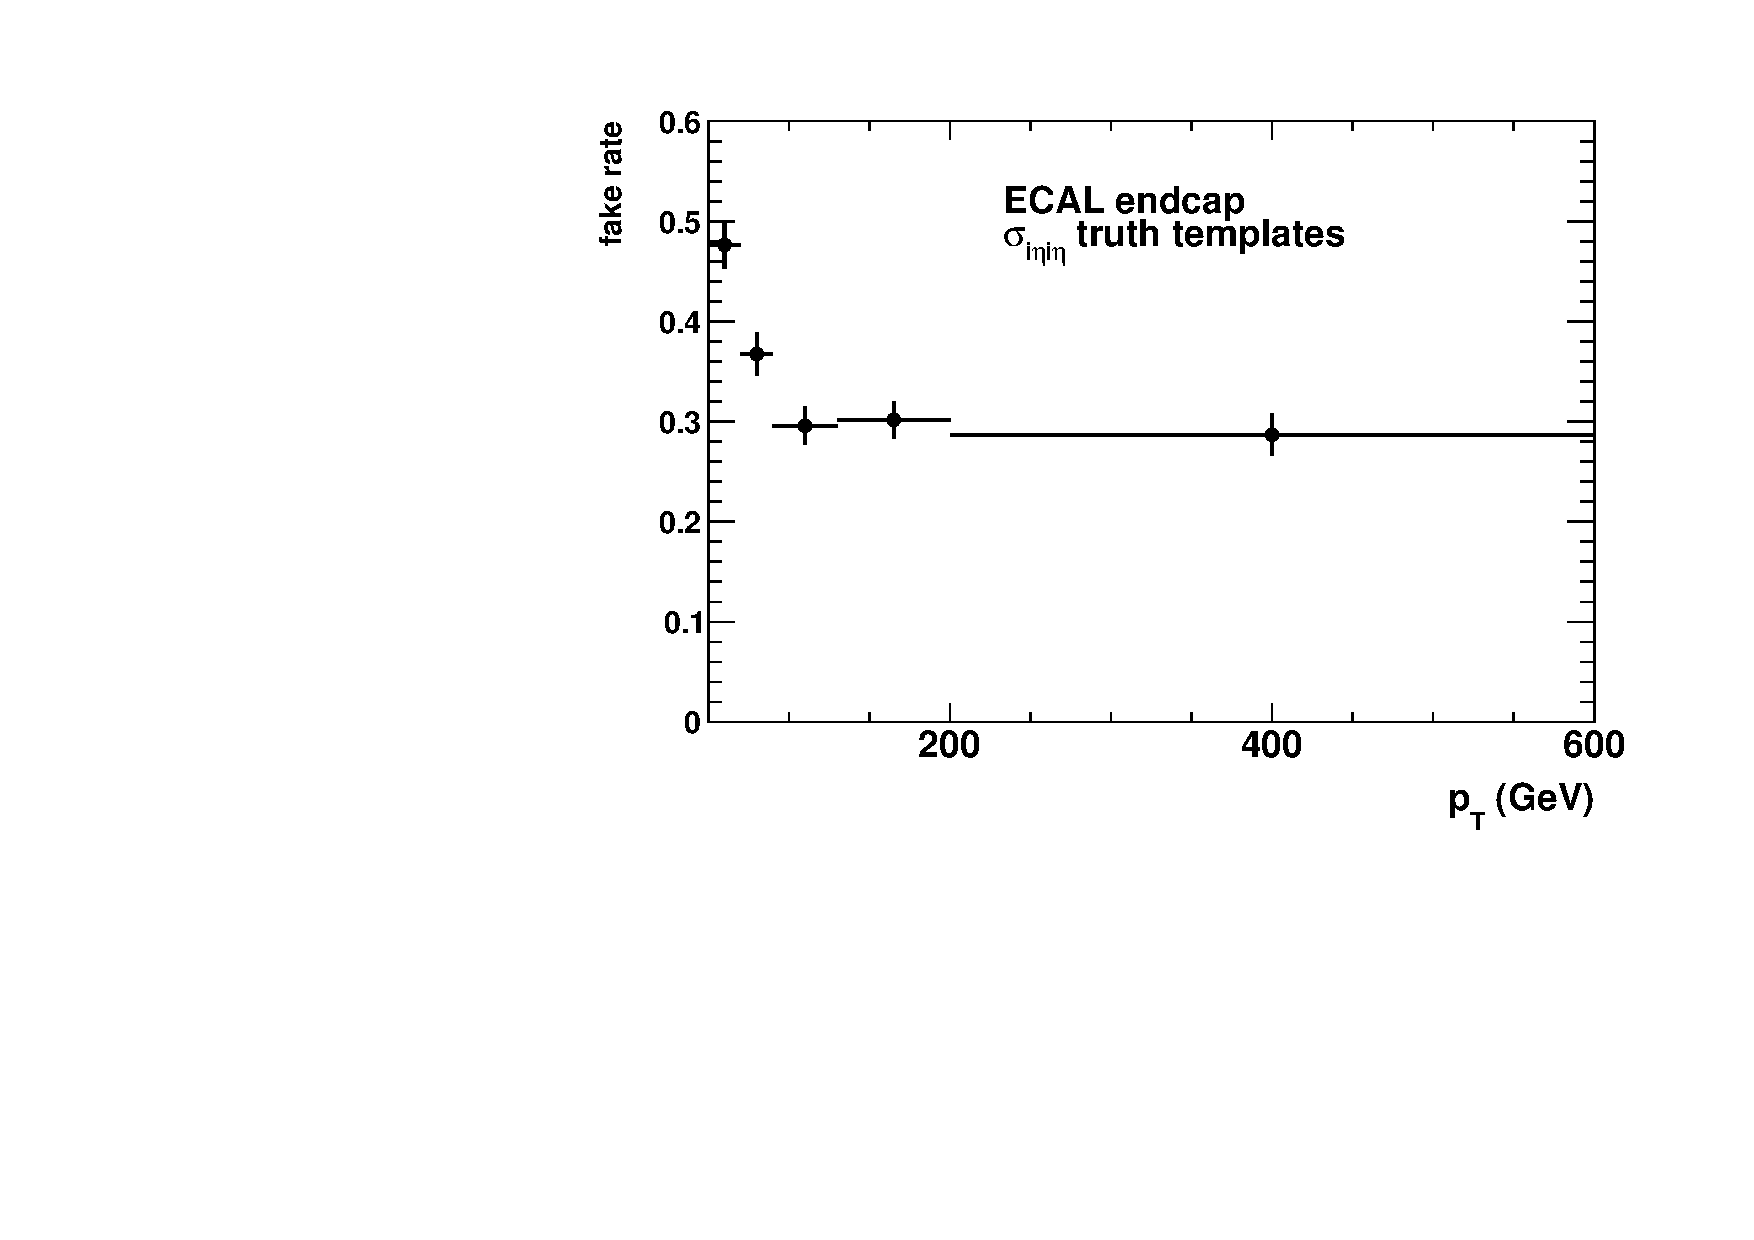
\includegraphics[scale=0.40]{figures/closure_test_EETruthFakeRate_sieie_chIso5To10.pdf}
  \caption{Fake rate derived using fake templates constructed using the MC truth information in the simulated sample as a function of \pt with \sieie templates in the EB (left) and EE (right) regions.}
  \label{fig:closure_test_fake_rates_sieie_truth}
\end{figure}


\subsubsection{Testing the Kinematics of Reweighted Denominator Objects}\label{sec:closure_test_kinematics}

The final step in the MC closure test is to verify that taking denominator objects (selected to be photon-like jets) and reweighting them by the fake rate does indeed produce an accurate representation of the kinematics of known fake events. This is to validate the final step of the actual fake background estimation technique used in the analysis where denominator objects are selected in the diphoton dataset and are reweighted by the fake rate measured in the jet-enriched dataset.

The fake rate for the MC sample is obtained by fitting a function of the same functional form as in Eq.~(\ref{eqn:fake_rate_fn}) to the MC fake rate derived using the nominal \chiso sideband selection, shown in Fig.~\ref{fig:closure_test_fake_rates_sieie}, separately in both the EB and EE. The fitted function and its associated fit parameters $p_0, p_1,$ and $p_2$ are shown in Fig.~\ref{fig:closure_test_fake_rate}. This function is used to reweight the denominator objects selected in the MC sample.

\begin{figure}[!htbp]
  \centering
  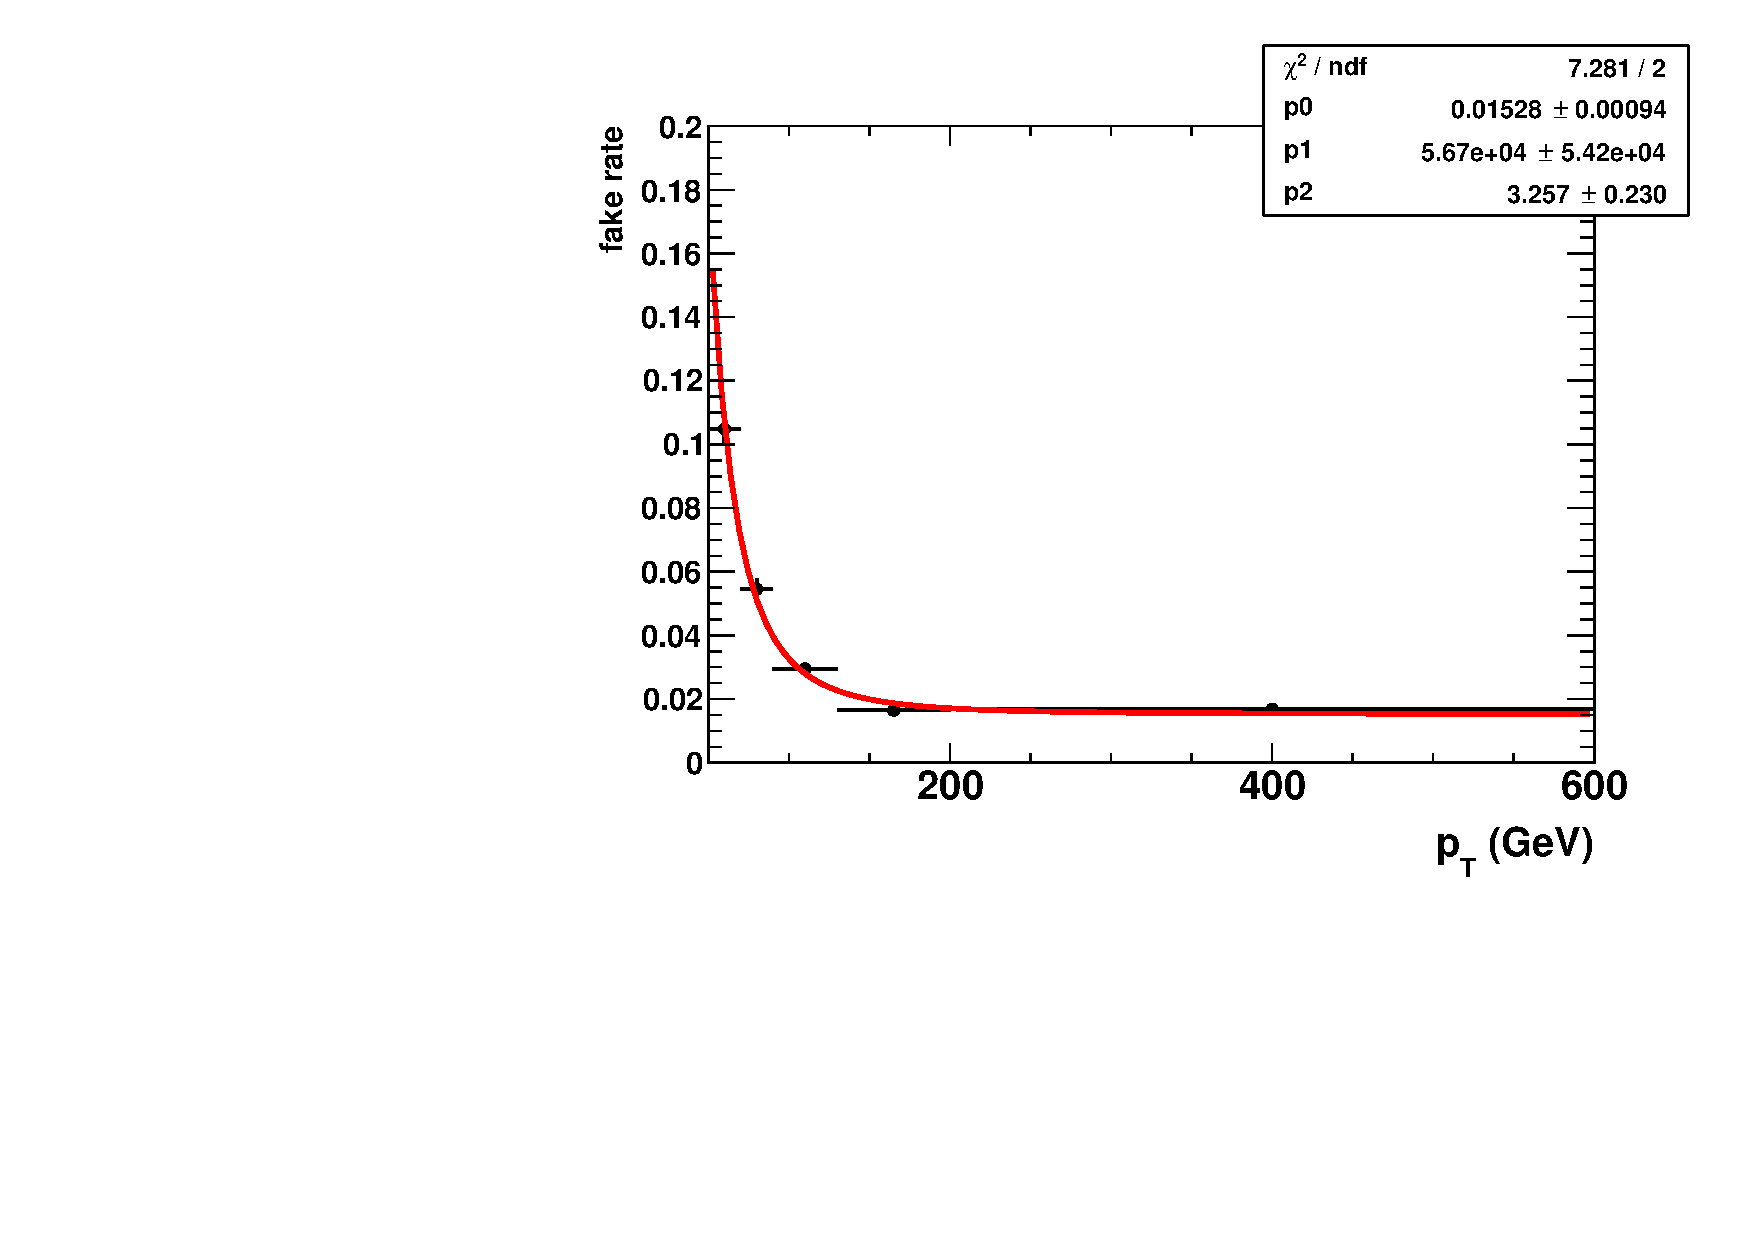
\includegraphics[scale=0.40]{figures/closure_test_fake_rate_fit_chIso5To10_EB.pdf}
  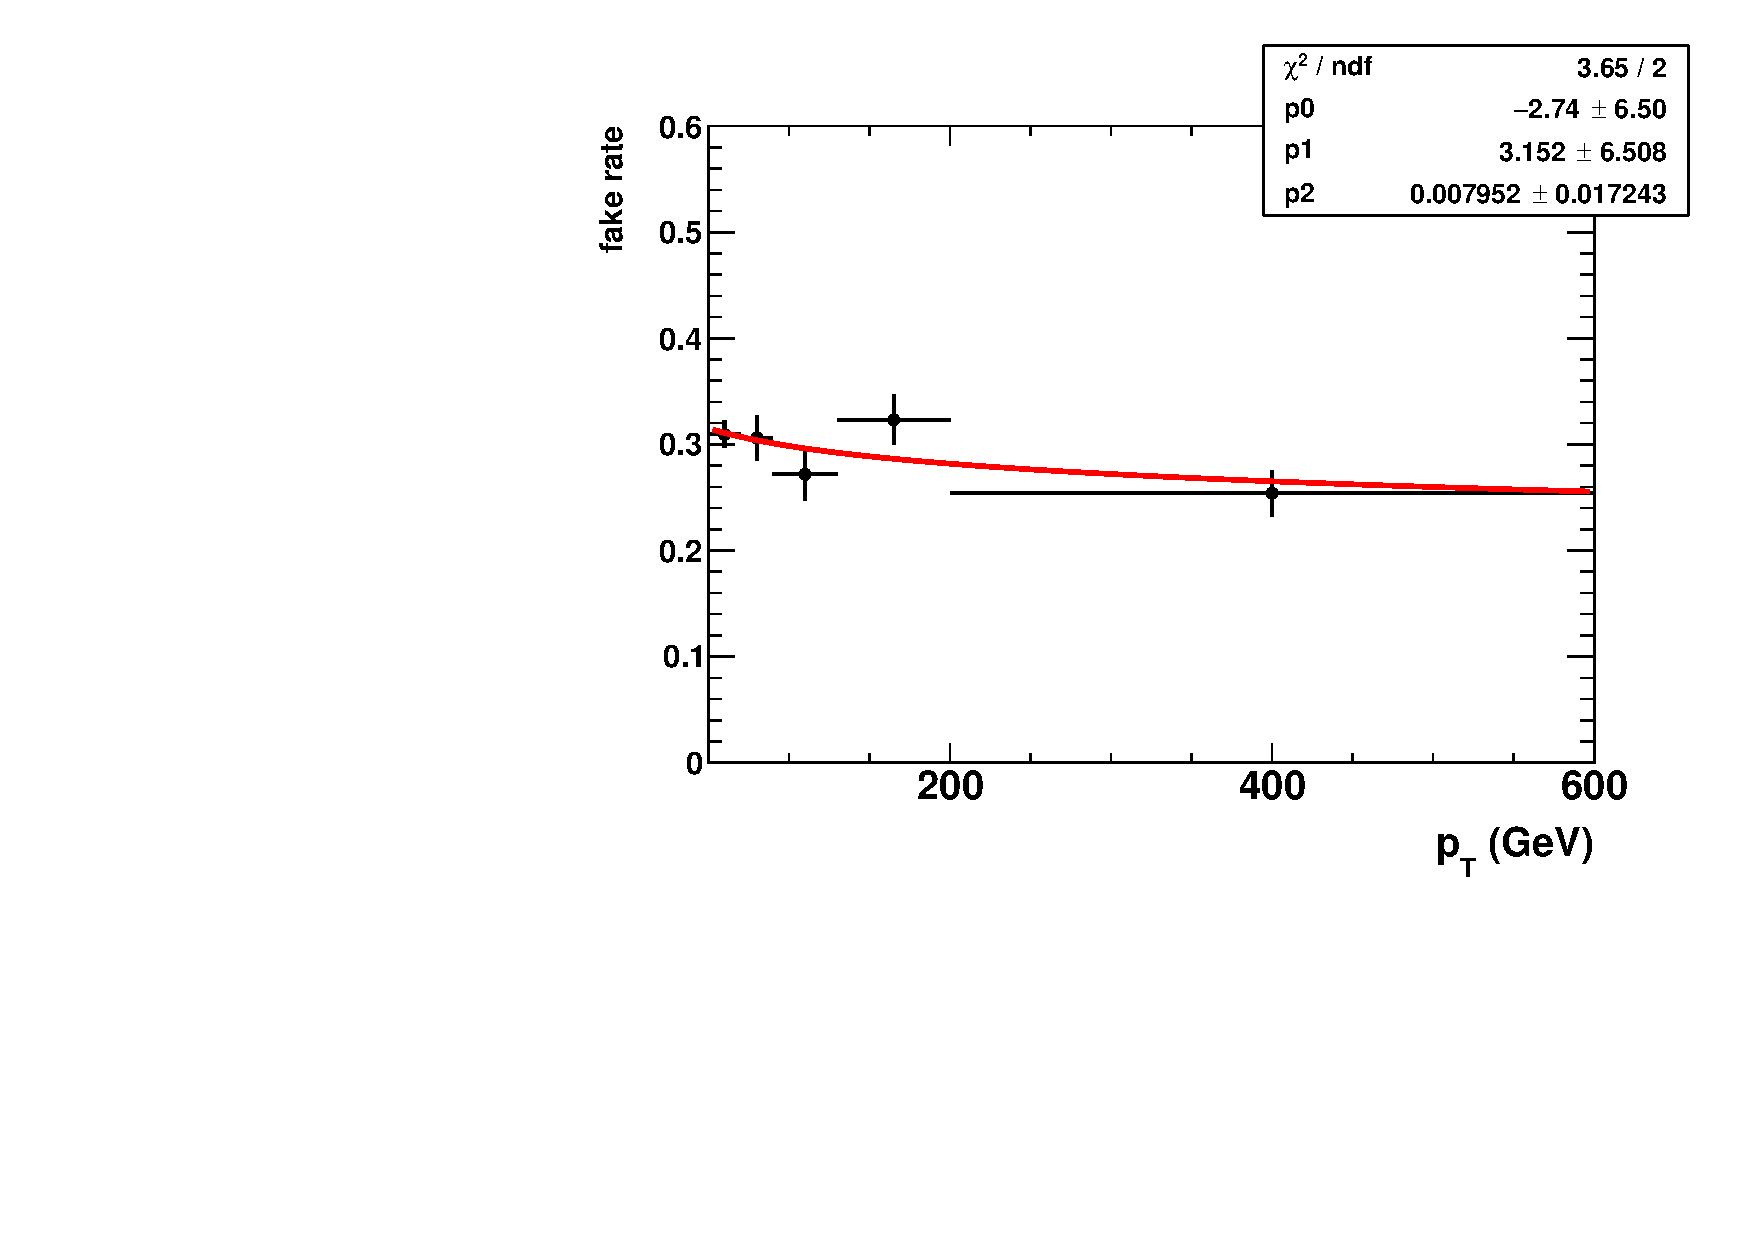
\includegraphics[scale=0.40]{figures/closure_test_fake_rate_fit_chIso5To10_EE.pdf}
  \caption{MC fake rate as a function of \pt in the EB (left) and EE (right) using the nominal \chiso sideband of 5-10\GeV.}
  \label{fig:closure_test_fake_rate}
\end{figure}

Fig.~\ref{fig:closure_test_photon_kinematics} shows the single photon kinematic variables \pt, $\eta$, and $\phi$ in the EB and EE regions for the MC denominator objects, the reweighted MC denominator objects, and distributions from the actual fakes in the MC sample determined using the MC truth information. Overall, the agreement is excellent in each region, but with better agreement in the EB than in the EE category. There are noticeable discrepancies at high values of $\eta$, but the level of disagreement is within the uncertainty ascribed to this fake rate method. With more statistics, this dependence could be accounted for by further subdividing the $\eta$ region and producing separate fake rates in each region, instead of just in the EB and EE regions.

\begin{figure}[!htbp]
  \centering
  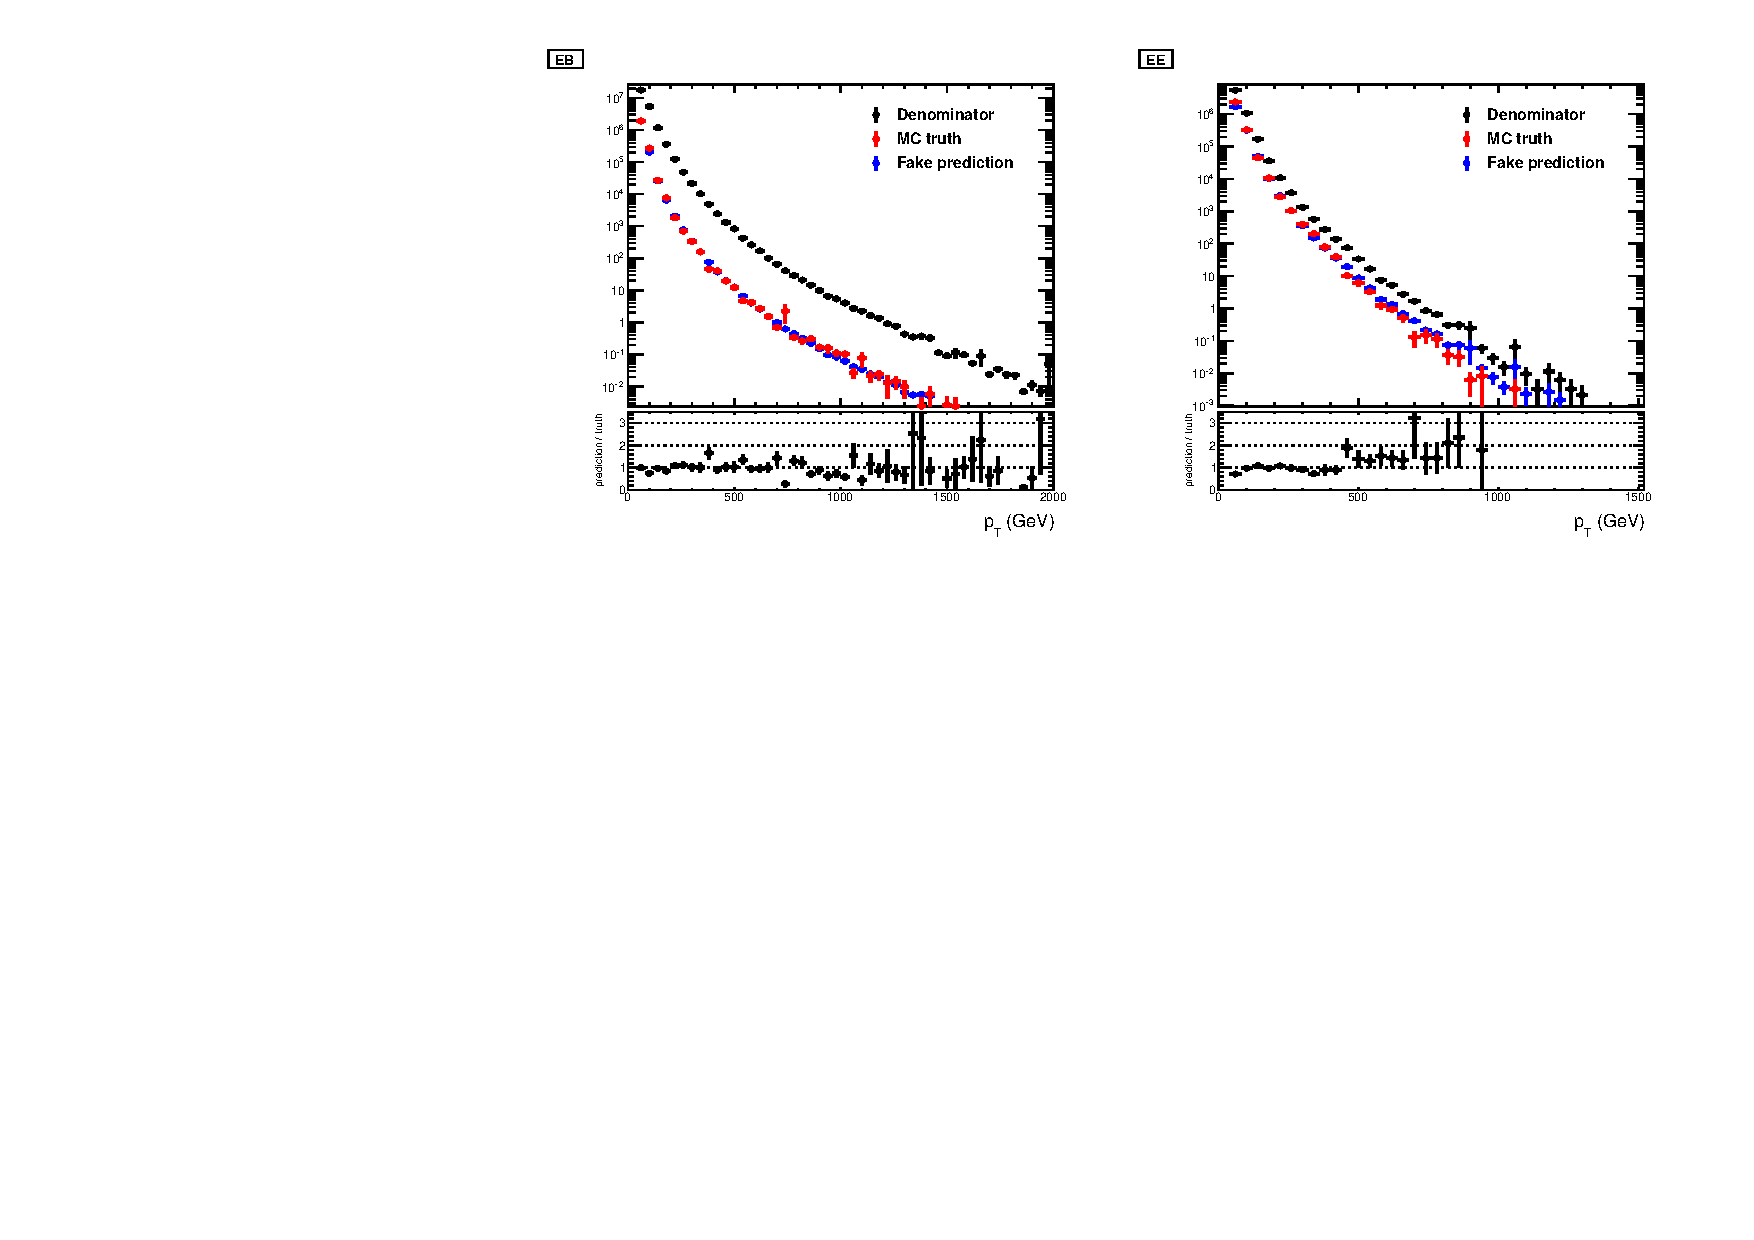
\includegraphics[scale=0.75]{figures/closure_test_photon_kinematics_pt.pdf}
  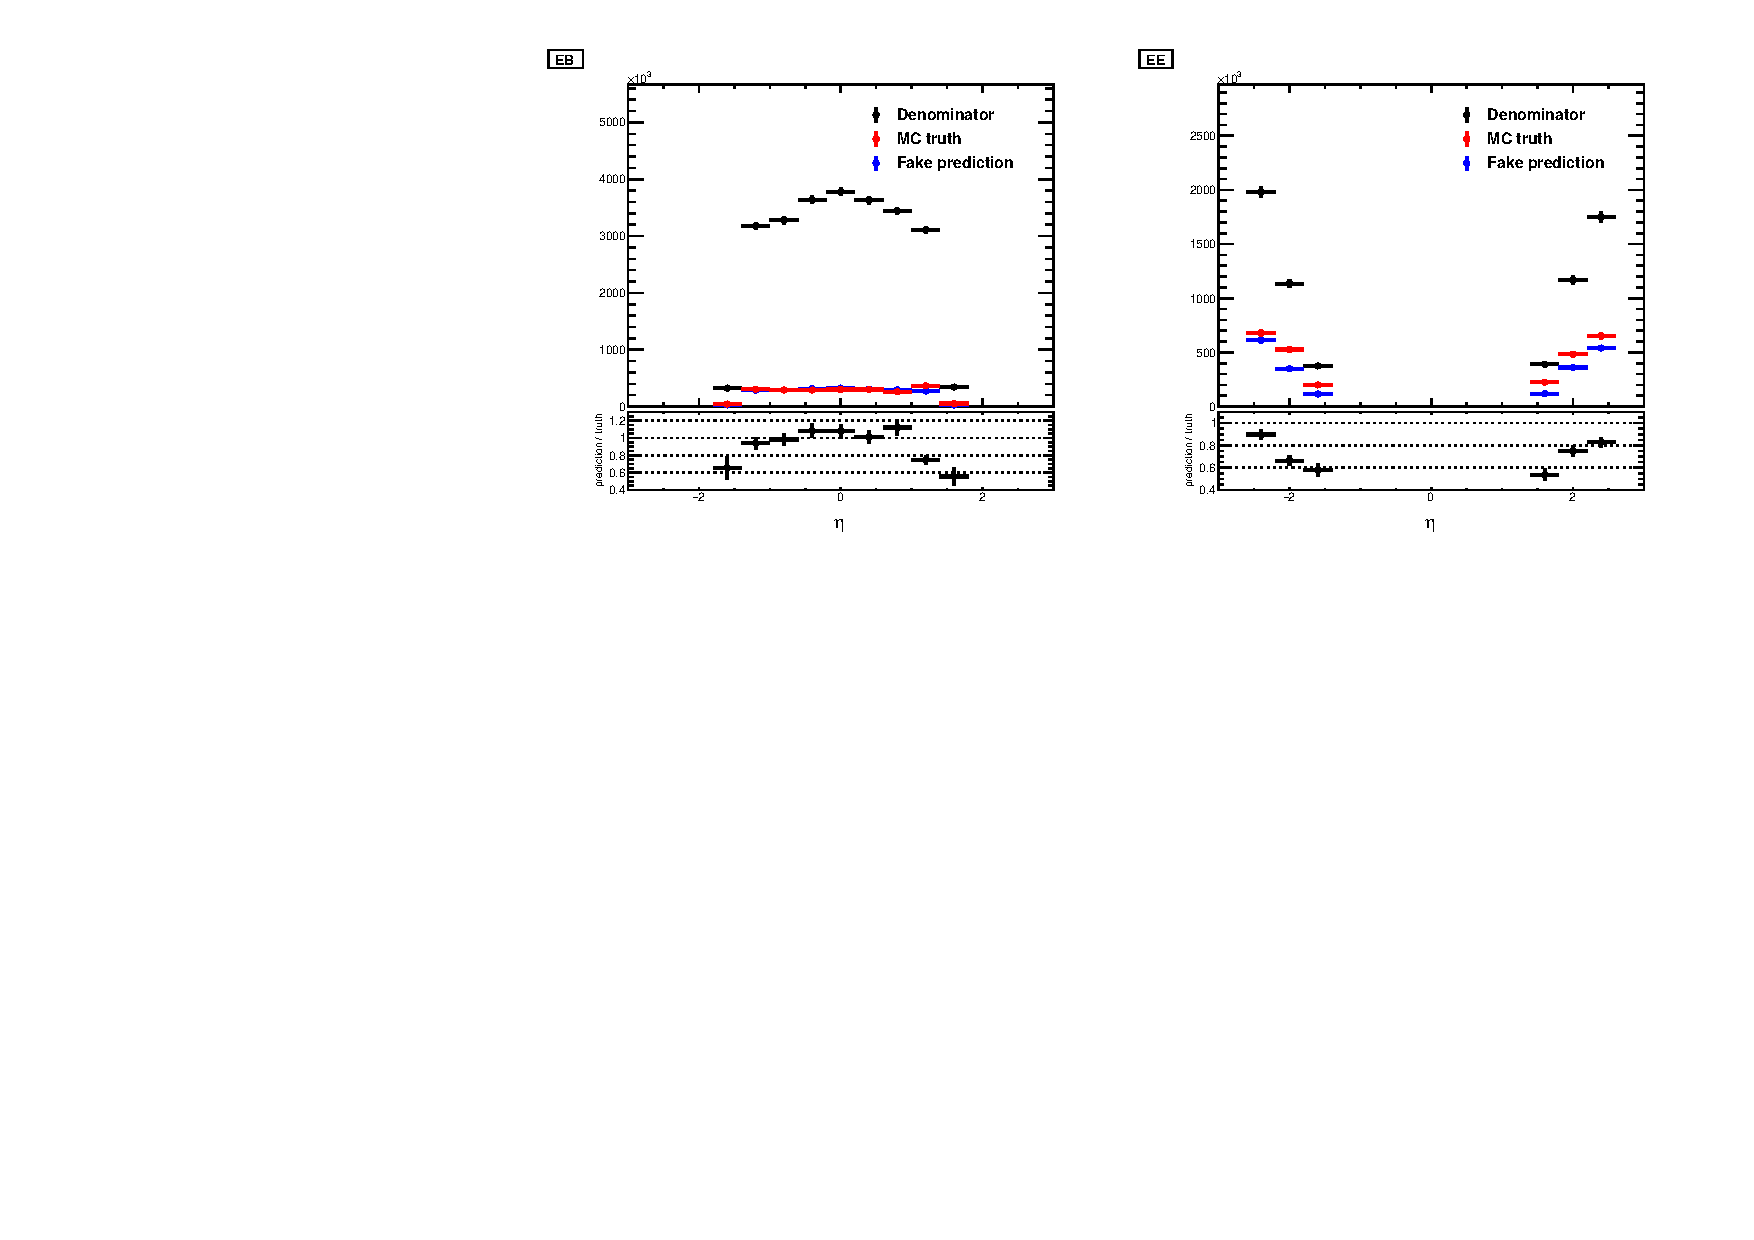
\includegraphics[scale=0.75]{figures/closure_test_photon_kinematics_eta.pdf}
  \includegraphics[scale=0.75]{figures/closure_test_photon_kinematics_phi.pdf}
  \caption{Closure test of the photon variables \pt (top), $\eta$ (middle), and $\phi$ (bottom) in the EB (left) and EE (right) regions. The MC denominator objects (black) are reweighted by the MC fake rate (blue) and compared against the distributions of known fakes identified using the MC truth (red).}
  \label{fig:closure_test_photon_kinematics}
\end{figure}

We also check the kinematics of the diphoton system. Diphotons are categorized in the EBEB, EBEE, EEEB, or EEEE regions depending on whether the leading or subleading photon is in the EB or EE. The \Mgg spectra are calculated using two real photons ($\gamma\gamma$), one real and one fake photon ($\gamma$j), or two fake photons (jj). Because the MC statistics are limited, we only compare the MC truth $\gamma$j spectra to the MC fake rate weighted $\gamma$j spectra, omitting the jj comparisons. These spectra are further categorized by whether the leading or subleading photons are real (T) or fake (F).

All possible categories using the $\gamma$j \Mgg distributions are merged to show the distribution as used in the main analysis, which combines the TF and FT ordering, drops the EEEE region, and merges the distinct EBEE and EEEB regions into the analysis-level EBEE category, as shown in Fig.~\ref{fig:closure_test_diphoton_kinematics_gjets}. The distributions for the individual categories of this type are shown in Fig.~\ref{fig:closure_test_diphoton_kinematics_TF_FT}. We can see that the diphoton invariant mass distribution obtained from events with denominator objects reweighted by the fake rate does indeed reproduce well the distribution that would be obtained for known fakes using the MC truth information.

\begin{figure}[!htbp]
  \centering
  \includegraphics[scale=0.70]{figures/closure_test_diphoton_kinematics_gjets_all.pdf}
  \caption{Closure test of the diphoton \Mgg distribution of $\gamma$j objects in the EBEB (left) and EBEE (right) categories. The MC denominator objects (black) are reweighted by the MC fake rate (blue) and compared against the distributions of known fakes identified using the MC truth (red).}
  \label{fig:closure_test_diphoton_kinematics_gjets}
\end{figure}

\begin{figure}[!htbp]
  \centering
  \includegraphics[scale=0.80]{figures/closure_test_diphoton_kinematics_TF_all.pdf}      
  \includegraphics[scale=0.80]{figures/closure_test_diphoton_kinematics_FT_all.pdf}
  \caption{Closure test of the diphoton \Mgg distribution of $\gamma$j objects ordered as TF (top 4 plots) and FT (bottom 4 plots) in the EBEB, EBEE, EEEB, and EEEE categories (specified in the plot titles). The MC denominator objects (black) are reweighted by the MC fake rate (blue) and compared against the distributions of known fakes identified using the MC truth (red).}
  \label{fig:closure_test_diphoton_kinematics_TF_FT}
\end{figure}


This concludes the MC closure test and demonstrates the validity of the photon fake rate method. Further studies involving different aspects of the closure test are discussed in the next section.


\subsection{Closure Test Studies}\label{ssec:closure_test_studies}


\subsubsection{Investigating the Change in Template Variable}

All aspects of the above closure test were done using \sieie as the template variable with fake templates derived using a \chiso sideband. We now repeat the closure test using the inverted relationship between these two variables, i.e., using \chiso as the template variable and \sieie as the sideband variable. The real templates constructed using the \chiso variable are formed from the simulated sample using the datasets listed in Table~\ref{tab:real_template_samples}, and Fig.~\ref{fig:real_templates_chiso} shows their evolution as a function of photon \pt. A nice feature of using this variable is that the templates are independent of photon \pt.

\begin{figure}[!htbp]
  \centering
  \includegraphics[scale=0.66]{figures/real_templates_chIso_overlaid_sample_all.pdf}
  \caption{Real templates in \chiso derived from simulation in the EB (left) and EE (right) categories for different photon \pt bins.}
  \label{fig:real_templates_chiso}
\end{figure}

Similarly, the fake templates constructed using the \chiso variable are formed from the simulated sample using the datasets listed in Table~\ref{tab:closure_test_samples}. The same sideband definitions for the \sieie variable that were used in the construction of the fake templates in Section~\ref{ss:fr_studies} are also used here. These definitions differ between the EB and EE regions. Fig.~\ref{fig:mc_fake_templates_fixed_pt_chiso} shows these fake templates compared to the distribution of MC truth fakes for $90 < \pt < 130\GeV$. The distributions using the other \pt bins considered in the closure test are shown in Appendix~\ref{sec:mc_fake_templates}. The expected bias in these templates is observed. We choose our nominal \sieie sideband to be 0.0105-0.0150 in the EB and 0.0280-0.0400 in the EE category. Using these choices, the \pt dependence of the \chiso fake templates is assessed and shown in Fig.~\ref{fig:mc_fake_templates_fixed_sideband_chiso}. These templates are also observed to be \pt independent.

\begin{figure}[!htbp]
  \centering
  \includegraphics[scale=0.40]{figures/closure_test_fake_template_chIso_EB_pt90To130_sample_all.pdf}
  \includegraphics[scale=0.40]{figures/closure_test_fake_template_chIso_EE_pt90To130_sample_all.pdf}
  \caption{Fake templates in \chiso using different \sieie sidebands from simulation for $90 < \pt < 130\GeV$ in the EB (left) and EE (right) categories, compared against the MC truth prediction.}
  \label{fig:mc_fake_templates_fixed_pt_chiso}
\end{figure}

\begin{figure}[!htbp]
  \centering
  \includegraphics[scale=0.66]{figures/closure_test_fake_templates_chIso_overlaid_sample_all}
  \caption{Fake templates from simulation using the nominal \sieie sidebands in the EB (left) and EE (right) categories for different \pt bins.}
  \label{fig:mc_fake_templates_fixed_sideband_chiso}
\end{figure}

Similar to the procedure done in the standard closure test, these templates were fit to numerator candidates using the simulated sample. Fig.~\ref{fig:closure_test_template_fit_chiso} shows an example fit using the nominal \sieie sideband choices in the EB and EE regions for $90 < \pt < 130\GeV$. The distributions using the other \pt bins are provided in Appendix~\ref{sec:mc_fake_rate_fits}. From the fits, we can extract the fake prediction in the simulated sample and derive a corresponding fake rate. This process was repeated using each of the sideband choices. The fake rates derived from each choice are compared against the yields of the MC truth fakes in Fig.~\ref{fig:closure_test_fake_rates_chiso}. There is some disagreement due to the mismodeling of the fakes by the fake templates. The ratio of the fake rate obtained using the nominal sideband choices to the MC truth fake rate is shown in Fig.~\ref{fig:closure_test_yields_chiso}. The final closure is about 30\% in the EB and 10\% in the EE category. 

\begin{figure}[!htbp]
  \centering
  \includegraphics[scale=0.66]{figures/{closure_test_h_pt90To130_sieie0.0105To0.0150_EB_Fake_chIso}.pdf}
  \includegraphics[scale=0.66]{figures/{closure_test_h_pt90To130_sieie0.0280To0.0400_EE_Fake_chIso}.pdf}
  \caption{An example template fit using the \chiso variable and nominal \sieie sidebands for the fake templates in the EB (top) and EE (bottom) categories with $90 < \pt < 130\GeV$.}
  \label{fig:closure_test_template_fit_chiso}
\end{figure}

\begin{figure}[!htbp]
  \centering
  \includegraphics[scale=0.40]{figures/closure_test_fake_rates_chIso_EB.pdf}
  \includegraphics[scale=0.40]{figures/closure_test_fake_rates_chIso_EE.pdf}
  \caption{The fake rate as a function of \pt using \chiso templates from simulation in the EB (left) and EE (right) categories with different \sieie sidebands, compared to the MC truth fake rate.}
  \label{fig:closure_test_fake_rates_chiso}
\end{figure}

\begin{figure}[!htbp]
  \centering
  \includegraphics[scale=0.40]{figures/closure_test_fake_rate_ratio_chIso_EB.pdf}
  \includegraphics[scale=0.40]{figures/closure_test_fake_rate_ratio_chIso_EE.pdf}
  \caption{Closure test of the event yields from the fake prediction in simulation using \chiso template fits compared to the MC truth yields in the EB (left) and EE (right) categories.}
  \label{fig:closure_test_yields_chiso}
\end{figure}

Next, we compare the above fake rates derived using the nominal sideband definitions to the ones obtained earlier using the \sieie templates. Both fake rates are shown in Fig.~\ref{fig:closure_test_fake_rates_comparison} and compared against the MC truth fake rate, separately in the EB and EE categories. There is good agreement among all three fake rates in both categories. For both template variables, the ratios of the predicted MC fake rates to the MC truth fake rate are given in Fig.~\ref{fig:closure_test_yields_comparison}. Both template choices largely agree within statistical uncertainty with some disagreement at low \pt in the EB. We stick with \sieie as the nominal template variable used for the fake rate method.

\begin{figure}[!htbp]
  \centering
  \includegraphics[scale=0.40]{figures/closure_test_fake_rates_comparison_EB.pdf}
  \includegraphics[scale=0.40]{figures/closure_test_fake_rates_comparison_EE.pdf}
  \caption{Comparison of the predicted MC fake rates as a function of \pt using \sieie (red) and \chiso (blue) templates in the EB (left) and EE (right) categories compared to the MC truth fake rate (gold).}
  \label{fig:closure_test_fake_rates_comparison}
\end{figure}

\begin{figure}[!htbp]
  \centering
  \includegraphics[scale=0.40]{figures/closure_test_fake_rate_ratio_comparison_EB.pdf}
  \includegraphics[scale=0.40]{figures/closure_test_fake_rate_ratio_comparison_EE.pdf}
  \caption{Closure test of the event yields from the fake prediction in the simulated sample using \sieie (blue) and \chiso (red) templates in the EB (left) and EE (right) regions.}
  \label{fig:closure_test_yields_comparison}
\end{figure}

A final study between these two template variables is a comparison of their predicted fake rates using the MC truth information to form their fake templates. These fake rates using the \sieie template variable were derived previously and shown in Section~\ref{ssec:closure_test}. The same procedure was repeated using the \chiso templates and the resulting fake rates are shown in Fig.~\ref{fig:truth_fake_rate_comparisons}, compared to the MC truth fake rate derived directly from the fake yields. All three of these are in excellent agreement, further validating the fitting procedure.

\begin{figure}[!htbp]
  \centering
  \includegraphics[scale=0.40]{figures/closure_test_fake_rates_truth_EB.pdf}
  \includegraphics[scale=0.40]{figures/closure_test_fake_rates_truth_EE.pdf}
  \caption{Fake rates derived using the MC truth information to construct fake templates in \sieie (red) and \chiso (blue) as a function of \pt in the EB (left) and EE (right) regions. These are compared against the MC fake rate derived from the fake yields (gold).}
  \label{fig:truth_fake_rate_comparisons}
\end{figure}


\subsubsection{Investigation of the Fake Composition from MC Truth}

In general, the fake templates using \sieie (see, e.g., Fig.~\ref{fig:mc_fake_templates_fixed_pt}) are peaked near the cut value of \sieie used in the high-\pt photon ID. This peak is usually expected for real photons and is more pronounced at low-\pt. We can see how isolated these reconstructed, known fake photons are by using the MC truth information available for the generated particles in the simulated sample used to select them.

Considering a region of $\Delta R < 0.1$ around the fake photons reveals that there are mostly two final state generated particles present, but often there are one, and sometimes, three particles. This does not depend on whether or not the fake photon passes the \sieie cut. Further investigation reveals that these final state generated particles mostly come from a single generated hadron mother, as expected. In the case of a single hadron mother producing a single final state generated particle, this creates a well isolated electromagnetic energy deposit (passing the \sieie cut) giving rise to the peak in the templates. When the single hadron mother decays to two final state generated particles, we need to consider their separation.

When there are two final state generated particles within a region of $\Delta R < 0.1$ from the fake reconstructed photon, we calculate their separation in $\Delta R$. This is done separately for the cases when the fake photon passes and fails the \sieie cut value of the photon ID. Fig.~\ref{fig:dR_study} shows this separation. A single crystal in the EB has a segmentation of $\Delta\eta{\times}\Delta\phi = 0.0174{\times}0.0174$. We see that most often these two particles are deposited within the same ECAL crystal, giving rise to a well isolated \sieie shower shape and contributing to the peak in the fake templates inside of the \sieie cut.

\begin{figure}[!htbp]
  \centering
  \includegraphics[scale=0.80]{figures/dR_cone_study_dR_two_particles.pdf}
  \caption{The separation in $\Delta R$ among two final state generated particles near a reconstructed fake photon in the EB (left) and EE (right) regions. The separation is shown separately for the fake photons that pass (black) and fail (red) the \sieie photon ID cut.}
  \label{fig:dR_study}
\end{figure}


\subsubsection{Real Photon Contamination}

We now check for possible contamination of real photons in the sideband, which is used to model fake photons, and in the denominator, which, unlike the numerator, is not corrected for. We check both cases separately, starting with the former.

Shown in Fig.~\ref{fig:sideband_cont} are the \sieie distributions in the EB and EE regions of different objects in the 5-10\GeV sideband from the simulated sample used in the closure test. Every reconstructed object in the sideband is matched to a generated particle using the MC truth information. A true source of fakes are those that are matched to a hadron mother. A true source of real photons are those that are matched to a hard scattering photon. There still remains some objects that are not matched and don't fall into either category. This mixture is predominantly fake-like (as can be inferred from their \sieie distribution) and are indicated as ``other" in Fig.~\ref{fig:sideband_cont} below. This plot shows that the fraction of real photons is small in the sideband. This small contamination is accounted for in using the variation of the sideband definition as a systematic uncertainty.

\begin{figure}[!htbp]
  \centering
  \includegraphics[scale=0.40]{figures/sieie_sideband_EB.pdf}
  \includegraphics[scale=0.40]{figures/sieie_sideband_EE.pdf}
  \caption{Composition of objects in the 5-10\GeV sideband in the simulated sample used for the closure test shown in the EB (left) and EE (right) categories. The fake (black) and fake-like (blue) objects dominate over the real (red) ones.}
  \label{fig:sideband_cont}
\end{figure}

Although the denominator objects are required to fail at least one of the photon ID variables, ensuring that the two categories are mutually exclusive, small contamination is still possible. To understand the real photon contamination in the denominator, we use the MC truth information available for the simulated sample used by the closure test. We take the reconstructed objects that pass the denominator definition and match them to a generated particle, as done above. Again, the real photons are those that are matched to a generated photon directly from the hard scattering. The fraction of these real photons over the total denominator objects as a function of \pt in the EB and EE categories is shown in Fig.~\ref{fig:denom_cont}. This contribution is less than 10\% over the majority of \pt range up to about 600\GeV. Although this fraction does rise with \pt, the effect is accounted for in the overall uncertainty attributed to the fake background.

\begin{figure}[!htbp]
  \centering
  \includegraphics[scale=0.35]{figures/pt_denominator_real_EB.png}
  \includegraphics[scale=0.35]{figures/pt_denominator_real_EE.png}
  \caption{The fraction of real photons among all denominator objects as a function of \pt, derived from the simulated sample used by the closure test in the EB (left) and EE (right) regions.}
  \label{fig:denom_cont}
\end{figure}



